\documentclass{report}
\usepackage{fullpage}
\usepackage{imakeidx}\makeindex
\usepackage[nottoc,notlot,notlof]{tocbibind}
\usepackage[toc]{glossaries}\makeglossaries
\usepackage{graphicx}
\usepackage{framed}
\usepackage{tcolorbox}
\usepackage{verbatim}
\usepackage{fancyvrb}
\usepackage{comment}
\usepackage{amsmath}
\usepackage{geometry}
\usepackage{enumitem}
\usepackage{etoolbox}
% \usepackage{bold-extra}
\usepackage{xcolor}
\usepackage[colorlinks=true, linkcolor=blue, urlcolor=blue, citecolor=violet]{hyperref}
\def\itemautorefname{Exercise}%
\def\chapterautorefname{Chapter}%
\def\figureautorefname{Figure}%
\def\sectionautorefname{Section}%

\AtBeginEnvironment{enumerate}{\everymath{\displaystyle}}
\newlist{problems}{enumerate}{2}
\setlist[problems]{wide=0pt}
\setlist[problems,1]{label=\thechapter.\arabic*, font=\bfseries, wide=0pt}
\setlist[problems,2]{label=(\alph*), wide =0.5em, topsep=2pt, itemsep=2pt}

\widowpenalty 10000
\clubpenalty 10000
\tolerance=9999
\newcommand{\tm}{\raisebox{.9ex}{\tiny tm}}

\newcommand{\harmonysource}[1]{
\begin{tabbing}
XX\=XXX\=XXX\kill
    \input{sources/#1.tex}
\end{tabbing}
}

\newcommand{\harmonylink}[1]{%
[\href{https://harmony.cs.cornell.edu/#1}{\underline{#1}}]%
}

\newcommand{\harmonyref}[2]{%
\href{https://harmony.cs.cornell.edu/output/#1}{\underline{#2}}%
}

\newglossaryentry{actor model}
{
  name=actor model,
  description={is a concurrency model where there are no shared variables, only
      threads with private variables that communicate through message passing}
}
\newglossaryentry{atomic instruction}
{
  name=atomic instruction,
  description={a machine instruction that may involve  multiple memory load and/or store
    operations and is executed atomically}
}
\newglossaryentry{atomicity}
{
  name=atomicity,
  description={describes that a certain machine instruction or sequence of machine
    instructions is executed indivisibly by a thread and cannot be interleaved with 
    machine instructions of another thread}
}
\newglossaryentry{barrier synchronization}
{
  name=barrier synchronization,
  description={is when a set of threads execute in rounds, waiting for one another
    to complete each round}
}
\newglossaryentry{blocked thread}
{
  name=blocked thread,
  description={is a thread that cannot change the state or terminate or
      can only do so after another thread changes the state first.
      For example, a thread that is waiting for a lock to become available}
}
\newglossaryentry{busy waiting}
{
  name=busy waiting,
  description={(aka spin-waiting) is when a thread waits in a loop for some
      application-defined condition instead of blocking}
}
\newglossaryentry{concurrent execution}
{
  name=concurrent execution,
  description={(aka parallel execution) is when there are multiple threads executing and
      their machine instructions are interleaved in an unpredictable manner}
}
\newglossaryentry{condition variable}
{
  name=condition variable,
  description={a variable that keeps track of which threads are waiting for a
    specific application-level condition.  The variable can be waited on as well
    as signaled or notified}
}
\newglossaryentry{context}
{
  name=context,
  description={(aka continuation) describes the state of a running thread,
    including its program counter, the values of its variables (stored in its
    register), and the contents of its stack}
}
\newglossaryentry{conditional critical section}
{
  name=conditional critical section,
  description={is a critical section with, besides mutual exclusion, additional conditions on
      when a thread is allowed to enter the critical section}
}
\newglossaryentry{critical section}
{
  name=critical section,
  description={(aka critical region) is a set of instructions that only one thread
    is allowed to execute at a time.  The instructions are, however, not executed
    atomically, as other threads can continue to execute and access shared
    variables}
}
\newglossaryentry{data race}
{
  name=data race,
  description={is when there are two or more threads concurrently accessing a
    shared variable, at least one of which is an update to the variable}
}
\newglossaryentry{deadlock}
{
  name=deadlock,
  description={is when there are two or more threads waiting indefinitely for one
    another to release a resource}
}
\newglossaryentry{determinism}
{
  name=determinism,
  description={is when the outcome of an execution is uniquely determined by the
    initial state}
}
\newglossaryentry{fairness}
{
  name=fairness,
  description={is when each thread eventually can access each resource it needs to access
    with high probability}
}
\newglossaryentry{invariant}
{
  name=invariant,
  description={is a binary predicate over states that must hold for every
  reachable state of a thread}
}
\newglossaryentry{linearizable}
{
  name=linearizable,
  description={is a consistency condition for concurrent access to an object, requiring
    that each access must appear to execute atomically sometime between the invocation
    of the access and its completion}
}
\newglossaryentry{lock}
{
  name=lock,
  description={an object that can be owned by at most one thread at a time.  Useful
    for implementing mutual exclusion}
}
\newglossaryentry{machine instruction}
{
  name=machine instruction,
  description={is an atomic operation on the Harmony virtual machine, executed by a thread}
}
\newglossaryentry{model checking}
{
  name=model checking,
  description={is a formal verification method that explores all possible executions
    of a program, which must have a finite number of states}
}
\newglossaryentry{monitor}
{
  name=monitor,
  description={is a programming language paradigm that supports mutual exclusion
    as well as waiting for resources to become available}
}
\newglossaryentry{mutual exclusion}
{
  name=mutual exclusion,
  description={is the property that two threads never enter the same critical section}
}
\newglossaryentry{non-blocking synchronization}
{
  name=non-blocking synchronization,
  description={(aka wait-free synchronization) is when access to a shared resource can be
      guaranteed in a bounded number of steps even if other threads are not making progress}
}
\newglossaryentry{sequential consistency}
{
  name=sequential consistency,
  description={is a consistency model in which shared memory accesses are
    executed in an order consistent with the program order}
}
\newglossaryentry{thread}
{
  name=thread,
  description={is code in execution.  We do not make the distinction
      between threads and threads.  A thread has a current context and
      updates its context every time it executes a machine instruction}
}
\newglossaryentry{thread variable}
{
  name=thread variable,
  description={is a variable that is private to a single thread and stored in
        its register}
}
\newglossaryentry{producer/consumer problem}
{
  name=producer/consumer problem,
  description={is a synchronization problem whereby one or more producing threads
    submit items and one or more consuming threads want to receive them.  No item
    can get lost or forged or be delivered to more than one consumer, and producers
    and consumers should block if resources are exhausted}
}
\newglossaryentry{property}
{
  name=property,
  description={describes a set of execution traces or histories that are allowed by
    a program.  Safety properties are properties in which ``no bad things happen,''
    such as violating mutual exclusion in a critical section.  Liveness properties are
    properties where ``something good eventually happens,'' like threads being
    able to enter the critical section if they want to}
}
\newglossaryentry{race condition}
{
  name=race condition,
  description={describes when multiple threads access shared state concurrently,
    leading to undesirable outcomes}
}
\newglossaryentry{reader/writer lock}
{
  name=reader/writer lock,
  description={is a lock on a resource that can be held by multiple threads if they all 
    only read the resource}
}
\newglossaryentry{semaphore}
{
  name=semaphore,
  description={is a counter that can be atomically incremented and decremented,
    but blocks the thread until the counter is larger than zero first}
}
\newglossaryentry{sequential execution}
{
  name=sequential execution,
  description={is when there is just one thread executing, as opposed to concurrent
    execution}
}
\newglossaryentry{shared variable}
{
  name=shared variable,
  description={is a variable that is stored in the memory of the Harmony virtual machine and
      shared between multiple threads, as opposed to a thread variable}
}
\newglossaryentry{spinlock}
{
  name=spinlock,
  description={is an implementation of a lock whereby a thread loops until the
    lock is available, at which point the thread atomically obtains the lock}
}
\newglossaryentry{stack machine}
{
  name=stack machine,
  description={is a model of computing where the state of a thread is kept on
    a stack.  Harmony uses a combination of a stack machine and a register-based machine}
}
\newglossaryentry{starvation}
{
  name=starvation,
  description={is when a thread cannot make progress because it is continuously
    losing a competition with other threads to get access to a resource}
}
\newglossaryentry{state}
{
  name=state,
  description={an assignment of values to variables.  In a Harmony virtual machine, this includes
      the contents of its shared memory and the set of contexts}
}
\newglossaryentry{step}
{
  name=step,
  description={is the execution of a machine instruction by a thread, updating
        its state.}
}
\newglossaryentry{thread safety}
{
  name=thread safety,
  description={is when the implementation of a data structure allows concurrent access
    with well-defined semantics}
}
\newglossaryentry{trace}
{
  name=trace,
  description={is a sequence of steps, starting from an initial state.  An infinite
    trace is also called a \emph{behavior}}
}

% \renewcommand{\topfraction}{.99}
% \renewcommand{\bottomfraction}{.99}
% \renewcommand{\textfraction}{.01}
% \renewcommand{\floatpagefraction}{.9}
% \renewcommand{\dbltopfraction}{.99}
% \renewcommand{\dblfloatpagefraction}{.9}

\newenvironment{code}{
\tcolorbox
}{
\endtcolorbox
}

\title{Concurrent Programming in Harmony}
\author{Robbert van Renesse}

\begin{document}
\begin{titlepage}
    \centering
    \vfill
    {\bfseries\huge
        Concurrent Programming in Harmony
    }
    \vfill
    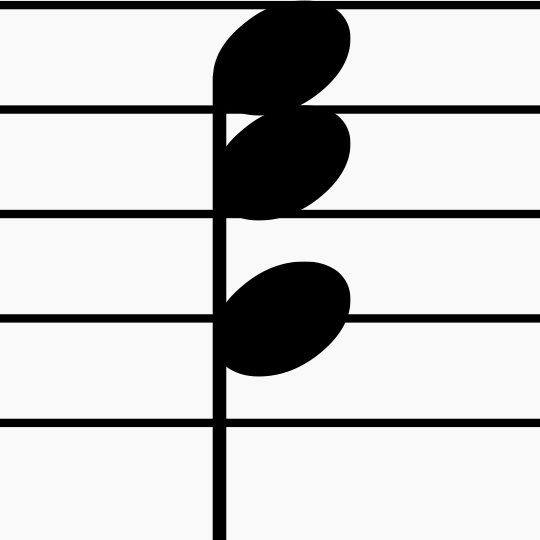
\includegraphics[width=6cm]{figures/harmony-icon.png}
    \vfill
    \vfill
    \hfill \Large Robbert van Renesse
\end{titlepage}

Permission is granted to copy, distribute and/or modify this
document under the terms of the
Creative Commons AttributionNonCommercial-ShareAlike 4.0 International
(CC BY-NC-SA 4.0) at
\url{http://creativecommons.org/licenses/by-nc-sa/4.0}.

\tableofcontents

\chapter{On Concurrent Programming}

Programming with concurrency is hard.  On the one hand concurrency
can make programs faster than sequential ones, but having multiple
\index{thread}%
threads read and update shared variables
\index{shared variable}%
concurrently and synchronize with one another makes programs more
complicated than programs where only one thing happens at a time.
%
\glsadd{concurrent execution}%
\glsadd{shared variable}%
\glsadd{sequential execution}%
\glsadd{determinism}%
\glsadd{atomicity}%
%
Why are concurrent
programs more complicated than sequential ones?
There are, at least, two reasons:
\begin{itemize}
\item The execution of a sequential
\index{sequential}%
program is mostly \emph{deterministic}.
\index{determinism}%
If you run it twice with the same input, the same output will be produced.
Bugs are typically easily reproducible and easy to track down, for example
by instrumenting the program.
On the other hand,
the output of running concurrent programs depends on how the
execution of the various threads are \emph{interleaved}.
Some bugs may occur only occasionally and
may never occur when the program is instrumented to find them
(so-called \emph{Heisenbugs}---overhead caused by instrumentation
leads to timing changes that makes such bugs less likely to occur).
\index{Heisenbug}%
\item In a sequential program, each statement and each function can be
thought of as happening \emph{atomically} (indivisibly)
\index{atomicity}%
because there is no other activity interfering with their execution.
Even though a statement or function may
be compiled into multiple machine instructions, they are executed back-to-back
until completion.  Not so with a concurrent program, where other threads
may update memory locations while a statement or function is being executed.
\end{itemize}
The lack of determinism and atomicity in concurrent programs make them
not only hard to reason about, but also hard to test.
\index{test}%
Running the same test of concurrent code twice is likely to produce
two different results.  More problematically, a test may trigger a
bug only for certain ``lucky'' executions.  Due to the probabilistic
nature of concurrent code, some bugs may be highly unlikely to get
triggered even when running a test millions of times.  And even if
a bug does get triggered, the source of the bug may be hard to find
because it is hard to reproduce.

\glsadd{model checking}%

This book is intended to help people with understanding and
developing concurrent code.  In particular, it uses a new tool
called Harmony that helps with \emph{testing} concurrent code.
The approach is based on \emph{model checking}:
\index{model checking}%
instead of relying
on luck, Harmony will run \emph{all possible executions} of a particular
test program.  So, even if a bug is unlikely to occur, if the test
\emph{can} expose the bug it \emph{will}.  Moreover, if the bug is
found, the model checker precisely shows how to trigger the bug in
the smallest number of steps.

Model checking is not a replacement for formal verification.
\index{formal verification}%
Formal verification proves that a program is correct.  Model checking only
verifies that a program is correct for some \emph{model}.  Think of
a model as a test program.
Because model checking tries every possible execution, the test
program needs to be simple. Otherwise it may take longer than we
care to wait for or run out of memory.
In particular, the model needs to have a relatively small number of
reachable states.

If model checking does not prove a program correct, why is it
useful?
To answer that question, let us consider a sorting algorithm.
Suppose we create a test program, a model, that tries sorting
\emph{all} lists of up to five numbers chosen from the set
\{ 1, 2, 3, 4, 5 \}.  Model checking proves that for those particular
scenarios the sorting algorithm works: the output is a sorted
permutation of the input.  In some sense it is an excellent test:
it will have considered all \emph{corner cases},
\index{corner case}%
including lists where all
numbers are the same, lists that are already sorted or reversely
sorted, etc.  If there is a bug in the sorting algorithm, most
likely it would be triggered and the model checker would produce a
scenario that would make it easy to find the source of the bug.

However, if the model checker does not find any bugs, we do not
know for sure that the algorithm works for lists of more than
five numbers or for lists that have values other than the numbers
1 through 5.  Still, we would expect that the likelihood that there
are bugs remaining in the sorting algorithm is small.
That said, it would be easy to write a program
that sorts all lists of up to five numbers correctly but fails to
do so for a list of 6 numbers.  (Hint: simply use an \textbf{if}
statement.)

\glsadd{invariant}%

While model checking does not in general prove an algorithm correct,
it can help with proving an algorithm correct.
The reason is that many correctness properties can be proved using
\emph{invariants}:
\index{invariant}%
predicates that must hold for every state in the
execution of a program.  A model checker can find violations of
proposed invariants when evaluating a model and provide valuable early
feedback to somebody who is trying to construct a proof, even an
informal one.
We will include examples
of such invariants as they often provide excellent insight into
why a particular algorithm works.

So, what is Harmony?
Harmony is a concurrent programming language.  It was designed to teach
the basics of concurrent programming, but it is also useful for
testing new concurrent algorithms or even sequential and distributed
algorithms.  Harmony programs are not intended to be ``run'' like programs
in most other programming languages---instead Harmony programs are
model checked to test that the program has certain desirable
properties and does not suffer from bugs.

The syntax and semantics of Harmony is similar to that of Python.
Python is familiar to many programmers and is easy to learn and
use.  We will assume that the reader is familiar with the basics
of Python programming.  We also will assume that the reader
understands some basics of machine architecture and how programs
are executed.  For example, we assume that the reader is familiar
with the concepts of CPU, memory, register, stack, and machine
instructions.

Harmony is heavily influenced by Leslie Lamport's work on
TLA+, TLC, and PlusCal~\cite{Lamport02, Lamport09},
Gerard Holzmann's work on Promela and SPIN~\cite{SPIN},
and University of Washington's DSLabs system~\cite{MWA19}.
Harmony is designed to have a lower learning curve than those
systems, but is not as powerful.  When you finish this book
and want to learn more, we strongly encourage checking
those out.
Another excellent resource is Fred Schneider's book ``On
Concurrent Programming''~\cite{Schneider97}.
(This chapter is named after that book.)

The book proceeds as follows:

\begin{itemize}
\item \autoref{ch:harmonyintro} introduces the Harmony programming
language, as it provides the language for presenting synchronization
problems and solutions.
\item \autoref{ch:concurrent} illustrates the problem of
concurrent programming through a simple example in which two threads
are concurrently incrementing a counter.
\item \autoref{ch:harmonymachine} presents the
Harmony virtual machine to understand the problem
underlying concurrency better.
\item \autoref{ch:critical} introduces the concept of a
\emph{critical section} and presents various flawed implementations
of critical sections to demonstrate that implementing a critical section
is not trivial.
\item \autoref{ch:peterson} introduces \emph{Peterson's Algorithm}, an
elegant (although not very efficient or practical) solution to implementating a critical section.
\item \autoref{ch:method} gives some more details on the Harmony
language needed for the rest of the book.
\item \autoref{ch:spinlock} introduces atomic \emph{locks}
for implemented critical sections.
\item \autoref{ch:synch} presents Harmony modules
that support locks and other synchronization primitives.
\item \autoref{ch:cds} gives an introduction to building concurrent
data structures.
\item \autoref{ch:testing} discusses approaches to testing
concurrent code in Harmony.
\item \autoref{ch:debugging} instead goes into how to find a bug
in concurrent code using the Harmony output.
\item \autoref{ch:condwait} talks about threads having to wait for
certain conditions.  As examples, it presents the reader/writer lock
problem and the bounded buffer problem.
\item \autoref{ch:sbs} presents \emph{Split Binary Semaphores}, a
general technique for solving synchronization problems.
\begin{comment}
\autoref{ch:rdwrbusy} also discusses \emph{busy-waiting}, which is
an easy but undesirable approach to synchronize threads.
\item \autoref{ch:semaphore} introduces \emph{semaphores},
a generalization of locks
that is good not only for mutual exclusion but also for waiting for
certain application-level conditions.
\item \autoref{ch:bb} and \autoref{ch:sbs} introduce the
\emph{bounded buffer problem} (aka \emph{producer/consumer problem})
and various solutions.
\end{comment}
\item \autoref{ch:starvation} talks about \emph{starvation}:
the problem that in some
synchronization approaches threads may not be able to get access to a
resource they need.
\item \autoref{ch:monitors} presents
\emph{monitors} and \emph{condition variables},
another approach to thread synchronication.
\item \autoref{ch:deadlock} describes \emph{deadlock}
where a set of threads are indefinitely waiting for one another to
release a resource.
\item \autoref{ch:actor} presents the \emph{actor model}
and \emph{message passing} as an approach to synchronization.
\item \autoref{ch:barrier} describes \emph{barrier synchronization},
useful in high-performance computing applications such as parallel simulations.
\item \autoref{ch:interrupts} discusses how to handle interrupts,
a problem closely related to---but not the same as---synchronizing threads.
\item \autoref{ch:nonblocking} introduces \emph{non-blocking} or
\emph{wait-free} synchronization algorithms,
which prevent threads waiting for one another more than a bounded number of
steps.
\item \autoref{ch:abp} presents a problem and a solution to the distributed
systems problem of having two threads communicate reliably over an unreliable
network.
\item \autoref{ch:leader} presents a protocol for electing a leader on
a ring of processors, where each processor is uniquely identified and 
only knows its successor on the ring.
\item \autoref{ch:2pc} describes atomic database transactions and the two-phase commit protocol used to implement them.
\item \autoref{ch:abd} presents a protocol for a fault-tolerant
replicated object that supports only read and write operations.
\item \autoref{ch:consensus} demonstrates a fault-tolerant distributed consensus
algorithm (aka protocol) expressed in Harmony.
\item \autoref{ch:paxos} shows how one can specify and check the well-known
Paxos consensus protocol.
\end{itemize}

\chapter{Introduction to Harmony}
\label{ch:harmonyintro}

Harmony is a programming language that borrows much of
Python's syntax.
Like Python, Harmony is an imperative,
dynamically typed, and garbage collected programming language.
There are also some important differences:
\begin{itemize}
\item Harmony only supports basic operator precedence or associativity.
Use parentheses liberally to remove ambiguity.
\item Harmony does not (currently) support floating point, iterators, or I/O;
Harmony does support \textbf{for} loops and various ``comprehensions.''
\item Python is object-oriented, supporting classes with methods and
inheritance; Harmony has objects but does not support classes.
On the other hand, Harmony supports pointers to objects and methods.
\end{itemize}
There are also less important ones that you will discover as
you get more familiar with programming in Harmony.

\begin{figure}
\begin{code}
\harmonysource{triangle}
\end{code}
\caption{\harmonylink{code/triangle.hny} Computing triangle numbers.}
\label{fig:triangle}
\end{figure}

\autoref{fig:triangle} shows a simple example of a Harmony program.
(The code for examples in this book can be found in the \texttt{code} folder under
the name listed in the caption of the example.)
The example is sequential and has a method \texttt{triangle} that takes
an integer number as argument.  Each method has a variable called
\textit{result} that eventually contains the result of the
method (there is no \textbf{return} statement in Harmony).  The method
also has a variable called \textit{n} containing the value of the
argument.  The \{ \textit{x..y} \} notation generates a set containing the numbers
from~\textit{x} to~\textit{y} (inclusive).
(Harmony does not have iterators and in particular does
not have a \texttt{range} operator.)
The last two lines in the program are
the most interesting.
The first assigns to \textit{x} some unspecified value in the range \texttt{0..N}
and the second verifies that $\mathtt{triangle}(x)$ equals $x(x+1)/2$.

``Running'' this Harmony program will try all possible executions, which
includes all possible values for $x$.  Try it out (here \texttt{\$}
represents a shell prompt):

\begin{code}
\begin{verbatim}
$ harmony triangle.hny
#states 13
13 components, 0 bad states
No issues
$
\end{verbatim}
\end{code}

(For this to work, make sure \texttt{harmony} is in your command shell's search path.)
Essentially, the $\texttt{choose}($S$)$
\index{choose operator}%
operator provides the input to the program by selecting some value from the
set~$S$, while the $\textbf{assert}$ statement checks that the output is
correct.  If the program is correct, the output of Harmony is the size of the
``state graph'' (13 states in this case).  If not, Harmony also
reports what went wrong, typically by displaying a summary of an execution in
which something went wrong.

In Harmony, constants have a default value,
but those can be overridden on the command
line using the \texttt{-c} option.
\index{constant}%
For example, if you want to test the code for \texttt{N = 100}, run:
\begin{code}
\begin{verbatim}
$ harmony -c N=100 triangle.hny
#states 103
103 components, 0 bad states
No issues
$
\end{verbatim}
\end{code}

\section*{Exercises}
\begin{problems}
\item See what happens if, instead of initializing \textit{result} to 0,
you initialize it to 1.  (You do not need to understand the error report at this time.  They will be explained in more detail in \autoref{ch:harmonymachine}.)
\item Write a Harmony program that computes squares by repeated adding.  So, the program
should compute the square of $x$ by adding $x$ to an initial value of 0 $x$ times.
\end{problems}

\chapter{The Problem of Concurrent Programming}
\label{ch:concurrent}

\begin{figure}[h]
\begin{center}
\begin{tabular}{ccc}
\begin{tcolorbox}[width=0.4\linewidth]
\harmonysource{prog1}
\end{tcolorbox}
& \rule{0.05\linewidth}{0in} &
\begin{tcolorbox}[width=0.4\linewidth]
\harmonysource{prog2}
\end{tcolorbox}
\\
(a) \harmonylink{code/prog1.hny} Sequential && (b) \harmonylink{code/prog2.hny} Concurrent
\end{tabular}
\end{center}
\caption{ A sequential and a concurrent program.}
\label{fig:progs}
\end{figure}

\glsadd{thread}%

Concurrent programming, aka multithreaded programming, involves multiple
threads
\index{thread}%
running in parallel while sharing variables.
\autoref{fig:progs} shows two programs.  Program (a) is sequential.
It sets \textit{shared} to \texttt{True}, asserts that
\textit{shared} = \texttt{True}, and finally sets
\textit{shared} to \texttt{False}.
If you run the program through Harmony, it will not find any problems
because there is only one execution possible and 1) in that execution
the assertion does not fail and 2) the execution terminates.
Program (b) is concurrent.  It executes methods \texttt{f()} and
\texttt{g()} in parallel.
If method \texttt{g()} runs and completes before \texttt{f()}, then
the assertion in \texttt{f()} will fail when \texttt{f()} runs.
Harmony will find this problem.
This problem is an example of non-determinism: methods \texttt{f()}
and \texttt{g()} can run in either order.

\autoref{fig:inc} presents a more subtle example that illustrates
non-atomicity.
The program initializes two shared variables:
an integer \textit{count} and
an array \textit{done} with two booleans.
The program then spawns two threads.
The first runs \texttt{incrementer(0)}; the second runs
\texttt{incrementer(1)}.

Method \texttt{incrementer} takes a parameter called \textit{self}.
It increments \textit{count} and sets \textit{done}[\textit{self}] to \texttt{True}.
It then waits until the other thread is done.
(\textbf{await} $c$ is shorthand for \textbf{while not} $c$: \textbf{pass}) and semantically the same.
After that, method \texttt{incrementer}
verifies that the value of \textit{count} equals~2.
% Like Python, Harmony supports \textbf{assert} statements with two arguments:
% the first is a Boolean condition, and the second is a value that is
% reported if the condition fails, in this case
% the value of \textit{count}.

Note that although the threads are \emph{spawned} one at a time,
they will execute concurrently.  It is, for example, quite possible
that \texttt{incrementer(1)} finishes before \texttt{incrementer(0)}
even gets going.
And because Harmony tries every possible execution, it will consider
that particular execution as well.
What would the value of \textit{count} be at the end of that execution?

\begin{figure}[h]
\begin{code}
\harmonysource{Up}
\end{code}
\caption{\harmonylink{code/Up.hny} Incrementing twice in parallel.}
\label{fig:inc}
\end{figure}

\begin{quote}
\begin{itemize}
\item Before you run the program, what do you think will happen?  Is the
program correct in that \textit{count} will always end up being 2?
(You may assume that \texttt{load} and \texttt{store} instructions of the
underlying virtual machine architecture are atomic (indivisible)---in fact
they are.)
\end{itemize}
\end{quote}

\glsadd{machine instruction}%

What is going on is that the Harmony program is compiled to machine instructions,
\index{machine instruction}%
and it is the machine instructions that are executed by the underlying Harmony
machine.  The details of this appear in \autoref{ch:harmonymachine},
but suffice it to
say that the machine has instructions that load values from memory and store
values into memory.  Importantly, it does not have instructions to atomically
increment or decrement values in shared memory locations.
So, to increment a value in memory,
the machine must do at least three machine instructions.  Conceptually:
\begin{enumerate}
\item load the value from the memory location;
\item add 1 to the value;
\item store the value to the memory location.
\end{enumerate}

When running multiple threads, each essentially runs an instantiation of
the machine, and they do so in parallel.  As they execute, their machine
instructions are interleaved
\index{interleaving}%
in unspecified and often unpredictable ways.
A program is correct if it works for any interleaving of threads.
Harmony will try all possible interleavings of the threads
executing machine instructions.

If the threads run one at a time, then \textit{count} will be incremented
twice and ends up being 2.  However, the following is also
a possible interleaving of \texttt{incrementer(0)} and \texttt{incrementer(1)}:
\begin{enumerate}
\item \texttt{incrementer(0)} loads the value of \textit{count}, which is 0;
\item \texttt{incrementer(1)} loads the value of \textit{count}, which is still 0;
\item \texttt{incrementer(1)} adds 1 to the value that it loaded (0), and
stores $1$ into \textit{count};
\item \texttt{incrementer(0)} adds 1 to the value that it loaded (0), and
stores $1$ into \textit{count};
\item \texttt{incrementer(0)} sets \textit{done}[0] to \texttt{True};
\item \texttt{incrementer(1)} sets \textit{done}[1] to \texttt{True}.
\end{enumerate}

The result in this particular interleaving is that \textit{count} ends up
being 1.
This is known as a \emph{race condition}.
\index{race condition}%
When running Harmony, it will
report violations of assertions.  It also provides an example
of an interleaving, like the one above, in which an assertion fails.

\glsadd{race condition}%

If one thinks of the assertion as providing the specification of the
program, then clearly its implementation does not satisfy its specification.
Either the specification or the implementation (or both) must have a bug.
We could change the specification by changing the assertion as follows:

\begin{code}
\textbf{assert} (\textit{count} == 1) or (\textit{count} == 2)
\end{code}

This would fix the issue, but more likely it is the program that must
be fixed, not the specification.

The exercises below have you try the same thing in Python.  As you will
see, the bug is not easily triggered when you run a Python version of
the program.  But in Harmony Murphy's Law applies:
if something can go wrong, it will.  Usually that is not a good thing,
but in Harmony it is.  It allows you to find bugs in your concurrent
programs much more easily than with a conventional programming language.

\section*{Exercises}

The following exercises are intended to show you that while it is just
as easy to write concurrent programs in Python, it is much easier to
find concurrency bugs using Harmony.

\begin{problems}
\item Harmony programs can usually be easily translated into Python.  For example,
\autoref{fig:incpy} is a Python version of \autoref{fig:inc}.
\begin{enumerate}
\item Run \autoref{fig:incpy} using Python.  Does the assertion fail?
\item Using a script, run \autoref{fig:incpy} 1000 times.
For example, if you are using the bash shell (in Linux or Mac OS X, say), you can do the following:
\begin{code}
\begin{verbatim}
for i in {1..1000}
do
    python Up.py
done
\end{verbatim}
\end{code}
If you're using Windows, the following batch script does the trick:
\begin{code}
\begin{verbatim}
FOR /L %%i IN (1, 1, 1000) DO python Up.py
PAUSE
\end{verbatim}
\end{code}
How many times does the assertion fail (if any)?
\end{enumerate}
\item \autoref{fig:incmany} is a version of \autoref{fig:incpy} that has each
incrementer thread increment \textit{count} \texttt{N} times.  Run \autoref{fig:incmany}
10 times (using Python).
Report how many times the assertion fails and what the value of \textit{count}
was for each of the failed runs.
Also experiment with lower values of \texttt{N}.
How large does \texttt{N} need to be for assertions to fail?
(Try powers of 10 for \texttt{N}.)
\item Can you think of a fix to \autoref{fig:inc}?  Try one or two different fixes
and run them through Harmony.  Do not worry about having to come up with a correct fix at this
time---the important thing is to develop an understanding of concurrency.
(Also, you do not get to use a \emph{lock}, yet.)
\end{problems}

\begin{figure}
\begin{code}
\VerbatimInput[xleftmargin=5mm,numbers=left]{../python/Up.py}
\end{code}
\caption{\harmonylink{python/Up.py} Python implementation of \autoref{fig:inc}.}
\label{fig:incpy}
\end{figure}

\begin{figure}
\begin{code}
\VerbatimInput[xleftmargin=5mm,numbers=left]{../python/UpMany.py}
\end{code}
\caption{\harmonylink{python/UpMany.py} Incrementing \texttt{N} times.}
\label{fig:incmany}
\end{figure}

\chapter{The Harmony Virtual Machine}
\label{ch:harmonymachine}
\index{Harmony Virtual Machine}%

Harmony programs are compiled to Harmony \emph{bytecode}
\index{bytecode}%
(a list of machine instructions for a virtual machine),
which in turn is executed by the Harmony virtual machine (HVM).
\index{virtual machine}%
\index{Harmony Virtual Machine}%
\index{HVM}%
The Harmony compiler places the bytecode for file $x$.\texttt{htm} in
file $x$.\texttt{hvm}.
The model checker, called \emph{Charm}, places its output in a file
called $x$.\texttt{hco} and a stylized version of the same output
in an HTML file called $x$.\texttt{htm}.

To understand the problem of concurrent computing, it
is important to have a basic understanding of machine instructions,
and in our case those of the HVM.

\section*{Harmony Values}

Harmony programs, and indeed the HVM,  manipulate Harmony values.
Harmony values are recursively defined:
they include booleans (\texttt{False} and \texttt{True}),
integers (but not floating point numbers),
strings (enclosed by double quotes),
sets of Harmony values,
and dictionaries
\index{dictionary}%
that map Harmony values to other Harmony values.
%
Another type of Harmony value is the \emph{atom}.
\index{atom}%
It is essentially
just a name.  An atom is denoted using a period followed by the
name.  For example, \texttt{.main} is an atom.

Harmony makes extensive use of dictionaries.
A dictionary maps keys to values.
Unlike Python, any Harmony value can be a key, including another
dictionary.
Dictionaries are written as
$\{ k_0: v_0, ~ k_1: v_1, ~ ... \}$.
If $d$ is a dictionary, and $k$ is a key, then the
following expression retrieves the Harmony value that $k$ maps to in $d$:
\begin{code}
$d$ $k$
\end{code}
The meaning of $d$ $a$ $b$ $...$ is ((($d$ $a$) $b$) $...$).
This notation is unfamiliar to Python programmers,
but in Harmony square brackets can be used
in the same way as parentheses, so you can express the same thing in the form
that is familiar to Python programmers:
\begin{code}
$d$[$k$]
\end{code}
However, if $d = \{ \mathtt{.count}: 3 \}$, then you can write
$d$.\texttt{count} (which has value 3) instead of having to write
$d$\texttt{[.count]} (although both will work).
Thus, using atoms, a dictionary can be made to look much like a Python object.

Tuples are special forms of dictionaries where the keys are
the indexes into the tuple.  For example, the tuple
\texttt{(5, False)} is the same Harmony value as
\texttt{\{ 0:5, 1:False \}}.
The empty tuple is written as \texttt{()}.
% Note that this is different from the empty set, which is \texttt{\{\}}.
As in Python, you can create singleton tuples by including a comma.
For example, \texttt{(1,)} is a tuple consisting just of the number 1.
Importantly, $(1) = 1 \ne (1,)$.

Again, square brackets and parentheses work the same in Harmony, so
\texttt{[a, b, c]} (which looks like a Python list)
is the same Harmony value as \texttt{(a, b, c)} (which looks like a Python tuple),
which in turn is the same Harmony value as \texttt{\{ 0:a, 1:b, 2:c \}}.
So, if $x$ = \texttt{[False, True]},
then $x$[0] = \texttt{False} and $x$[1] = \texttt{True}, just like in Python.
However, when creating a singleton list, make sure you include the
comma, as in \texttt{[False,]}.  The expression \texttt{[False]} just means
\texttt{False}.

Harmony is not an object-oriented language, so objects don't have
built-in methods.  However, Harmony does have some powerful operators to
make up for some of that.
For example, dictionaries have two handy unary operators.
If $d$ is a
dictionary, then \texttt{keys}~$d$ (or equivalently \texttt{keys}($d$))
returns the set of keys and \texttt{len}~$d$ returns the size of
this set.

\autoref{ap:values} provides details on all the values that
Harmony currently supports.

\section*{Harmony Bytecode}

A Harmony program is translated into HVM bytecode.
To make it amenable to efficient model checking,
the HVM is not an ordinary virtual machine, but its architecture
is nonetheless representative of conventional computers and
virtual machines such as the Java Virtual Machine.

Instead of bits and bytes, a HVM manipulates Harmony values.
A HVM has the following components:
\begin{itemize}
\item Code:  This is an immutable and finite list of HVM instructions,
generated from a Harmony program.  The types of instructions will be described later.
\item Shared memory: A HVM has just one memory location containing
a Harmony value.
\item Threads:  Any thread
can spawn an unbounded number of other threads and threads may terminate.
Each thread has a program counter that indexes into the code,
\index{program counter}%
a stack of Harmony values,
and two private \emph{registers} that each contain a Harmony value.
\index{register}%
\end{itemize}

\glsadd{context}%
\index{thread-local}%
One of the registers of a thread contains the local variables of the
method that the thread is currently executing.  It is saved and restored by
method invocations.  The other register is called \textbf{this} and is
used for so-called \emph{thread-local state}, which contains variables that
can be used by all methods.
The state of a thread is called a \emph{context} (aka \emph{continuation}):
\index{context}%
\index{continuation}%
it contains the values of its program counter, stack, and registers.
The state of a HVM
consists of the value of its memory and the multiset (or \emph{bag})
\index{bag}%
\index{multiset}%
of contexts.  It is a multiset of contexts because two threads can
have the same context.

\begin{figure}
\begin{code}
\begin{verbatim}
   0 Frame __init__ ()
code/Up.hny:1 count = 0
   1 Push 0
   2 Store count
code/Up.hny:2 done = [ False, False ]
   3 Push [False, False]
   4 Store done
code/Up.hny:4 def incrementer(self):
   5 Jump 32
   6 Frame incrementer self
code/Up.hny:5     count = count + 1
   7 Load count
   8 Push 1
   9 2-ary +
   10 Store count
code/Up.hny:6     done[self] = True
   11 Push ?done
   12 LoadVar self
   13 Address
   14 Push True
   15 Store
code/Up.hny:7     await done[1 - self]
   16 Push 1
   17 LoadVar self
   18 2-ary -
   19 Load done
   20 Apply
   21 JumpCond False 16
code/Up.hny:8     assert count == 2
   22 ReadonlyInc
   23 AtomicInc
   24 Load count
   25 Push 2
   26 2-ary ==
   27 Load count
   28 Assert2
   29 AtomicDec
   30 ReadonlyDec
   31 Return
\end{verbatim}
\end{code}
\caption{The first part of the HVM bytecode corresponding to \autoref{fig:inc}.}
\label{fig:inccode}
\end{figure}

It may seem strange that there is only one memory location.
However, this is not a limitation because Harmony values are unbounded trees.
The shared memory is a dictionary that maps atoms (names of shared
variables) to other Harmony values.
We call this a \emph{directory}.
\index{directory}%
Thus, a directory represents the state of a collection of variables named
by the atoms.
%
Because directories are Harmony values themselves,
directories can be organized into a tree.
Each node in a directory tree is then identified
by a sequence of Harmony values, like a path name in the file system
hierarchy.  We call such a sequence an \emph{address}.
\index{address}%
For example, in \autoref{fig:inc} the memory is a dictionary with two
entries: \texttt{.count} and \texttt{.done}.  And the value of entry
\texttt{.done} is a dictionary with keys 0 and 1.
So, for example, the address of \texttt{done[0]} is the sequence
[ \texttt{.done}, 0 ].
An address is itself a Harmony value.

\glsadd{stack machine}%

Compiling the code in \autoref{fig:inc} results in the HVM bytecode
listed in \autoref{fig:inccode}.
You can obtain this code by invoking \texttt{harmony} with the \texttt{-a} flag
like so:
\begin{code}
\begin{verbatim}
harmony -a Up.hny
\end{verbatim}
\end{code}
Each thread in the HVM is predominantly a \emph{stack machine},
\index{stack machine}%
but it also has two registers.
Like shared memory, the registers usually contain dictionaries so they
can represent the values of multiple named variables.
As mentioned before, one register contains a dictionary with the local
variables of the method that the thread is currently executing,
while the other contains thread-local state.

\index{sequential consistency}%
All instructions are atomically executed.
The Harmony memory model is \emph{sequentially consistent}: all
accesses are in program order.
Most instructions pop values from the stack or push values onto the stack.
At first there is one thread, named \texttt{\_\_init\_\_},
which initializes the state.
It starts executing at instruction 0 and keeps executing until
it reaches the last instruction in the program.
In this case, it executes instructions 0 through 5 first.
The last instruction in that sequence is a \texttt{JUMP}
instruction that sets the program counter to 32
(skipping over the code for \texttt{incrementer} method).
The \texttt{\_\_init\_\_} thread then executes instructions
32 through 40 and finishes.
Once initialization completes, any threads that were spawned
(in this case \texttt{incrementer(0)} and \texttt{incrementer(1)})
can run.

\begin{figure}
\begin{code}
\begin{verbatim}
#states 32
Safety Violation
T0: __init__() [0-5,32-40] { count: 0, done: [ False, False ] }
T1: incrementer(0) [ 6- 9] { count: 0, done: [ False, False ] }
T2: incrementer(1) [ 6-18] { count: 1, done: [ False, True  ] }
T1: incrementer(0) [10-28] { count: 1, done: [ True,  True  ] }
Harmony assertion failed: 1
open file:///Users/rvr/github/harmony/harmony.html for more information
\end{verbatim}
\end{code}
\caption{The text output of running Harmony on \autoref{fig:inc}.}
\label{fig:incoutput}
\end{figure}

At program counter 6 is the code for the \texttt{incrementer} method.
All methods start with a \texttt{Frame} instruction and end with a
\texttt{Return} instruction.
\autoref{ap:harmonybytecode} provides a list of all HVM machine instructions,
in case you want to read about the details.
The \texttt{Frame} instruction lists the name of the method and the
names of its arguments.
The code generated from $\mathit{count} := \mathit{count} + 1$ in line~5 of
\texttt{Up.hny} is as follows (see \autoref{fig:inccode}):

\begin{enumerate} \setcounter{enumi}{6}
\item The \texttt{Load} instruction pushes the value of the
\textit{count} variable onto the stack.
\item The \texttt{Push} instruction pushes the constant 1
onto the stack of the thread.
\item \texttt{2-ary} is a \texttt{+} operation with 2 arguments.
It pops two values from the stack (the value of \textit{count} and 1),
adds them, and pushes the result back onto the stack.
\item The \texttt{Store} instruction pops
a Harmony value (the sum of the \textit{count} variable and 1) and
stores it in the \textit{count} variable.
\end{enumerate}

You can think of Harmony as trying every possible interleaving of threads executing
instructions.
\autoref{fig:incoutput} shows the output produced by running Harmony on the
\texttt{Up.hny} program.

Harmony can report the following failure types:
\begin{itemize}
\item \texttt{Safety violation}: This means something went wrong with
at least one of the executions of the program that it tried.  This
can include a failing assertion, divide by zero, using an uninitialized
or non-existent variable, dividing a set by an integer, and so on.
% It also includes certain infinite loops.
Harmony will print a trace of the shortest bad execution that it found.
\item \texttt{Non-terminating State}: Harmony found one or more states
from which there does not exist an execution such that all threads
terminate.  Harmony will not only print the non-terminating state with
the shortest trace, but also the list of threads
at that state, along with their program counters.
\item \texttt{Active Busy Waiting}:  There are states in which
some thread cannot make progress without the help of another thread but
does not block;
\item \texttt{Data Race}: There are states in which two or more threads
concurrently access a shared variable, at least one of which is a store
operation.
% \item \texttt{Stopped States}: Similar to non-terminating states,
% these are states in which some threads are left that cannot
% terminate.  \autoref{ch:synch} will explain what it means for
% a thread to be stopped.
\end{itemize}

Harmony checks for these types of failure conditions in the given
order: if there are multiple failure conditions, only the first is
reported.  \emph{Active busy waiting} (\autoref{ch:condwait}) is not
technically an indication of a synchronization problem, but instead an
indication of an inefficient solution to a synchronization problem---
one that uses up significantly CPU cycles.
A \emph{data race} (\autoref{ch:synch}) may not be a bug either---whether or
not it is might depend on the semantics of the underlying memory
operations and are therefore generally undesirable.

Going back to our example, Harmony reports a safety violation.
In particular, it reports that the assertion failed
because \textit{count} has value 1 instead of 2.
Next it reports an execution that failed this assertion.
The program got to the failed assertion in 4 ``turns.''
The output has four columns:
\begin{enumerate}
\item A thread identifier;
\item The main method and argument of the thread;
\item The sequence of program counters of the HVM instructions that the thread executed;
\item The contents of the shared memory.
\end{enumerate}

\begin{figure}
\begin{center}
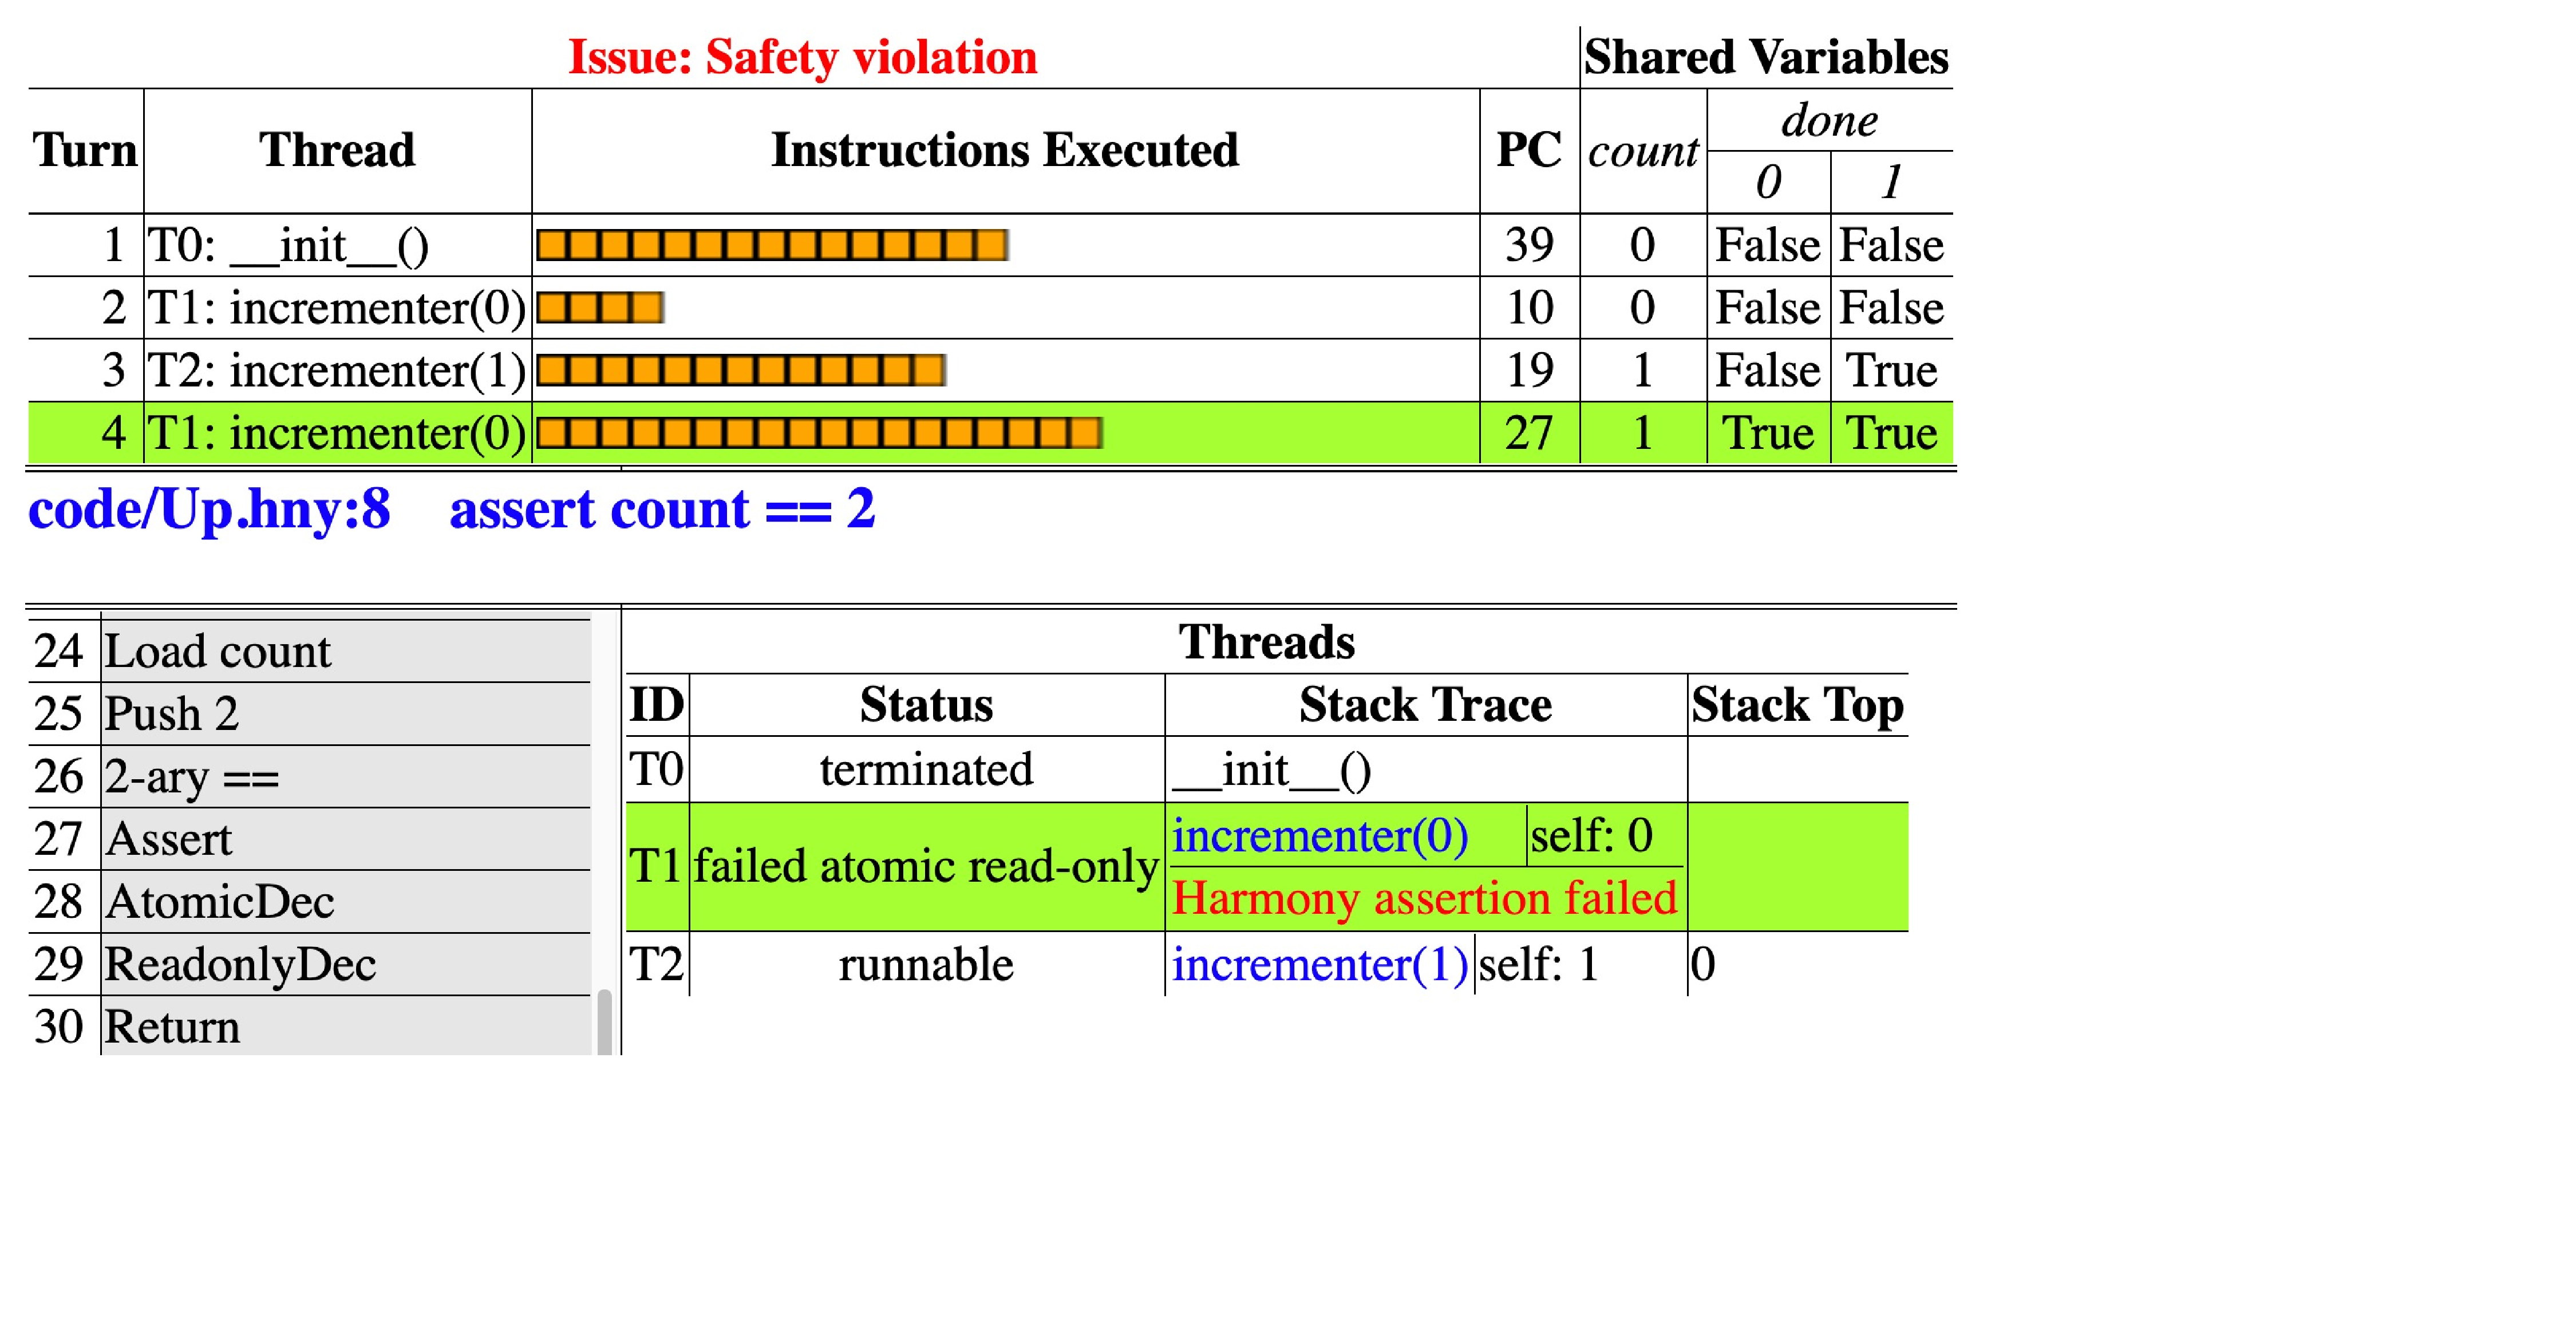
\includegraphics[width=0.9\textwidth]{figures/Up1.pdf}
\end{center}
\caption{The
\harmonyref{Up.html}{HTML output of running Harmony on \autoref{fig:inc}}.
There are four sections.
The top shows the turns to the problematic state.
Each turn shows a thread identifier, the method the thread is executing,
a ``timeline'' containing a block for each instruction executed, the
program counter of the thread, and the values of the shared variables
at those turns.
The middle section shows the line of code that is being executed.
The bottom left shows the bytecode of the program.
The bottom right shows the state of each thread.
Each row in the stack trace of a thread shows
the method that is being evaluated and
the values of its method variables.}
\label{fig:inchtml1}
\end{figure}

The four turns in the execution are as follows:

\begin{enumerate}
\item Thread \texttt{\_\_init\_\_} (with identifier T0)
sets shared variable \textit{count} to 0 and
shared variable \textit{done} to \texttt{[False, False]}.
\item Thread \texttt{incrementer(0)} (with identifier T1)
executes instructions 6 through 9, loading the value of
\textit{count} but stopping just before storing 1 into \textit{count};
\item Thread \texttt{incrementer(1)} (with identifier T2)
executes instructions 6 through 18, storing 1 into
\textit{count} and storing \texttt{True} into \textit{done}[1];
\item Thread \texttt{incrementer(0)}
continues execution, executing instructions 10 through 28
storing value 1 into \textit{count} (instruction 10),
storing \texttt{True} into \textit{done}[0] (instructions 11 through 15)
finding that \textit{done}[1] is \texttt{True} (instructions 16 through 21),
and finally detecting that the assertion is violated
(instructions 22 through 28).
\end{enumerate}

Harmony also generates an HTML file that allows exploring more details
of the execution interactively.
Open the suggested HTML file and you should see something like
\autoref{fig:inchtml1}.

In the top right, the HTML file contains the reported issue in red.
Underneath it, a table shows the four turns in the execution.
Instead of listing explicitly the program counters of the executed
instructions, the HTML file contains a list of blocks for each
executed instruction.  We call this the \emph{timeline}.
You can click on such a block to see the state of the Harmony
virtual machine just after executing the corresponding instruction.
The turn that is being executed is highlighted in green.
The table also lists the program counter of the thread at each turn,
and the values of the shared variables.

Underneath the table it shows the line of Harmony code that is being
executed in blue.

The bottom left shows
the bytecode of the program being executed.  It has alternating
grey and white sections.  Each section corresponds to a line of
Harmony code.  The instruction that is about to be executed,
if any, is highlighted in red.  (In this case, the state shown
is a failed state and no instruction will be executed next.)
If you hover the mouse over a machine instruction, it provides a
brief explanation of what the instruction does.

The bottom right contains a table with the state of each thread.
The thread that is executing is highlighted in green.
Status information for a thread can include:
\begin{itemize}
\item[] \texttt{runnable}: the thread is runnable but not
currently running.  In Harmony, threads are interleaved and so
at most one thread is actually running;
\item[] \texttt{running}: the thread is currently executing
instructions;
\item[] \texttt{terminated}: the thread has completed all its
instructions;
\item[] \texttt{failed}: the thread has encountered an error,
such as violating an assertion or divide by zero;
\item[] \texttt{blocked}: the thread cannot make progress until
another thread has updated the shared state.  For example, this
occurs when one of the implementers is waiting for the other
to set its \textit{done} flag;
\item[] \texttt{atomic}: the thread is in \emph{atomic} mode,
not allowing other threads to be scheduled.  This is, for example,
the case when an assertion is being checked;
\item[] \texttt{read-only}: the thread is in \emph{read-only} mode,
not able to modify shared state.  Assertions can execute
arbitrary code including methods, but they are not allowed to
modify the shared state.
\end{itemize}

The stack of each thread is subdivided into two parts: the
\emph{stack trace} and the \emph{stack top}.
A stack trace is a list of methods that are being invoked.
In this case, the \texttt{incrementer} method does not invoke any
other methods, and so the list is of length 1.
For each entry in the stack trace, it shows the method name and
arguments, as well as the variables of the method.
The stack top shows the values on the stack beyond the stack trace.

When you load the HTML file, it shows the state after executing
the last instruction.
As mentioned above, you can go to any point in the execution by
clicking on one of the blocks in the timeline.
There are also various handy keyboard shortcuts:
\begin{tabular}{rl}
\emph{Right arrow}: & go to the next instruction; \\
\emph{Left arrow}: & go to the previous instruction; \\
\emph{Down arrow}: & go to the next turn; \\
\emph{Up arrow}: & go to the previous turn; \\
\emph{Enter (aka Return)}: & go to the next line of Harmony code; \\
\emph{0}: & go to the initial state.
\end{tabular}

If you want to see an animation of the entire execution, one instruction
at a time, you can first hit 0 and then hold down the right arrow.
If you want to see it one line of Harmony code at a time, hold down the
enter (aka return) key instead.
If you hold down the down arrow key, the movie will
go by very quickly.

\section*{Exercises}

\begin{problems}
\item \autoref{fig:incenter} shows an attempt at trying to fix the code of
    \autoref{fig:inc}.  Run it through Harmony and see what happens.  Based on
    the error output, describe in English what is wrong with the code by describing,
    in broad steps, how running the program can get into a bad state.
\item What if we moved line~5 of \autoref{fig:incenter} to after the \textbf{if}
    statement (between lines~7 and~8)?  Do you think that would work?  Run it through
    Harmony and describe either why it works or why it does not work.
\end{problems}

\begin{figure}
\begin{code}
\harmonysource{UpEnter}
\end{code}
\caption{\harmonylink{code/UpEnter.hny} Broken attempt at fixing the code of \autoref{fig:inc}.}
\label{fig:incenter}
\end{figure}

\chapter{Critical Sections}
\label{ch:critical}

\begin{figure}
\begin{code}
\harmonysource{csbarebones}
\end{code}
\caption{\harmonylink{code/csbarebones.hny} A bare bones critical section with two threads.}
\label{fig:csbarebones}
\end{figure}

\begin{figure}
\begin{code}
\harmonysource{cs}
\end{code}
\caption{\harmonylink{code/cs.hny} Harmony model of a critical section.}
\label{fig:cs}
\end{figure}

Hopefully you have started thinking of how to solve the concurrency
problem and you may already have prototyped some solutions.
In this chapter we will go through a few reasonable but broken attempts.
At the heart of the problem is that we would like make sure that, when
the \textit{count} variable is being updated, no other thread is
trying to do the same thing.  This is called a \emph{critical section}
(aka critical region)~\cite{EWD123}:
a set of instructions where only one thread is allowed to execute at a
time.
\index{critical section}%
\index{critical region}%

\glsadd{critical section}%
\glsadd{thread safety}%

Critical sections are useful when accessing a shared data
structure, particularly when that access requires multiple underlying
machine instructions.  A counter is a very simple example of
a data structure, but as we have seen it too requires multiple instructions.
A more involved one would be accessing a binary tree.
Adding a node to a binary tree, or re-balancing a tree, often requires
multiple operations.  Maintaining ``consistency'' is certainly much easier
if during this time no other
thread also tries to access the binary tree.
Typically, you want some invariant property of the data structure to hold
at the beginning and at the end of the critical section, but in the middle
the invariant may be temporarily broken---this is not a problem as critical
sections guarantee that no other
thread will be able to see it.
An implementation of a data structure that can be safely accessed by multiple
threads and free of race conditions is called \emph{thread-safe}.
\index{thread safety}%
\index{thread}%

\glsadd{mutual exclusion}%

A critical section is often modeled as threads in an infinite loop
entering and exiting the critical section.
\autoref{fig:csbarebones} shows the Harmony code.
Here \texttt{@cs} is a \emph{label},
\index{label}%
identifying a location in the HVM bytecode.  The first thing we need to
ensure is that there can never be two threads in the critical section.
This property is called \emph{mutual exclusion}.
\index{mutual exclusion}%
We would like to place an assertion at the \texttt{@cs} label that
specifies that only the current thread can be there.

Harmony in fact supports this.
It has an operator \textbf{atLabel}~$L$,
\index{atLabel operator}%
where $L$
is the atom containing the name of the label (in this case, \texttt{cs}).
The operator returns a bag (multiset) of (method, argument) pairs of threads
executing at that label.
In our case there are two threads: \texttt{(thread, 0)} and \texttt{(thread, 1)}.
A bag is represented by a dictionary that maps each element
in the bag to the number of times the element appears in the bag.
Method \textbf{atLabel} only exists for specification purposes---do not
use it in normal code.
If you run the code through Harmony, the assertion should fail because
there is no code yet for safely entering and exiting the critical section.

However, mutual exclusion by itself is easy to ensure.
For example, we could insert the following code to enter the
critical section:
\begin{code}
\texttt{await False}
\end{code}
This code will surely prevent two or more threads from being
at label \texttt{@cs} at the same time.
But it does so by preventing \emph{any} thread from reaching
the critical section.
We clearly need another property besides mutual exclusion.

Mutual exclusion is an example of a \emph{safety property},
\index{safety property}%
a property that ensures that \emph{nothing bad will happen}, in this case
two threads being in the critical section.
What we need now is a \emph{liveness property}:
\index{liveness property}%
we want to ensure that
\emph{eventually something good will happen}.
There are various possible liveness properties we could use,
but here we will propose the following informally: if
(1) there exists a non-empty
set $S$ of threads that are trying to enter the critical section and
(2) threads in the critical section always leave eventually, then
eventually one thread in $S$ will enter the critical section.
We call this \emph{progress}.
\index{progress}%

In order to detect violations of progress, and other liveness problems in
algorithms in general, Harmony requires that every execution must be
able to reach a state in which all threads have terminated.
Clearly, even if mutual exclusion holds in \autoref{fig:csbarebones},
the spawned threads never terminate.  We
will instead model threads in critical sections using the framework in
\autoref{fig:cs}: a thread can \emph{choose} to enter a
critical section more than once, but it can also choose to terminate, even
without entering the critical section ever.
(Recall that Harmony will try every possible execution, and so it will evaluate
both choices.)

\begin{comment}
\begin{figure}
\begin{center}
\includegraphics[width=3.5in]{figures/mutex-crop.pdf}
\end{center}
\caption{High-level state diagram specification of mutual exclusion with up to two threads.
The first number in a state gives the number of threads; the second number is the
number of threads in the critical section.}
\label{fig:mutex}
\end{figure}

\autoref{fig:mutex} shows a high-level state diagram
\index{state diagram}%
of mutual exclusion and progress.
The circles represent states, while the arrows represent possible state
transitions (high-level steps).  The label in each circle summarizes the state;
the label on an arrow describes the transition.  In this case,
the label contains two numbers: the total number of threads and the number
of threads in the critical section.
\end{comment}

A thread that is in the critical
section cannot terminate until after leaving the critical section.
We will now consider various approaches toward implementing this
specification.

\begin{figure}
\begin{code}
\harmonysource{naiveLock}
\end{code}
\caption{\harmonylink{code/naiveLock.hny} Na\"{\i}ve implementation of a shared lock.}
\label{fig:naivelock}
\end{figure}

\begin{figure}
\begin{center}
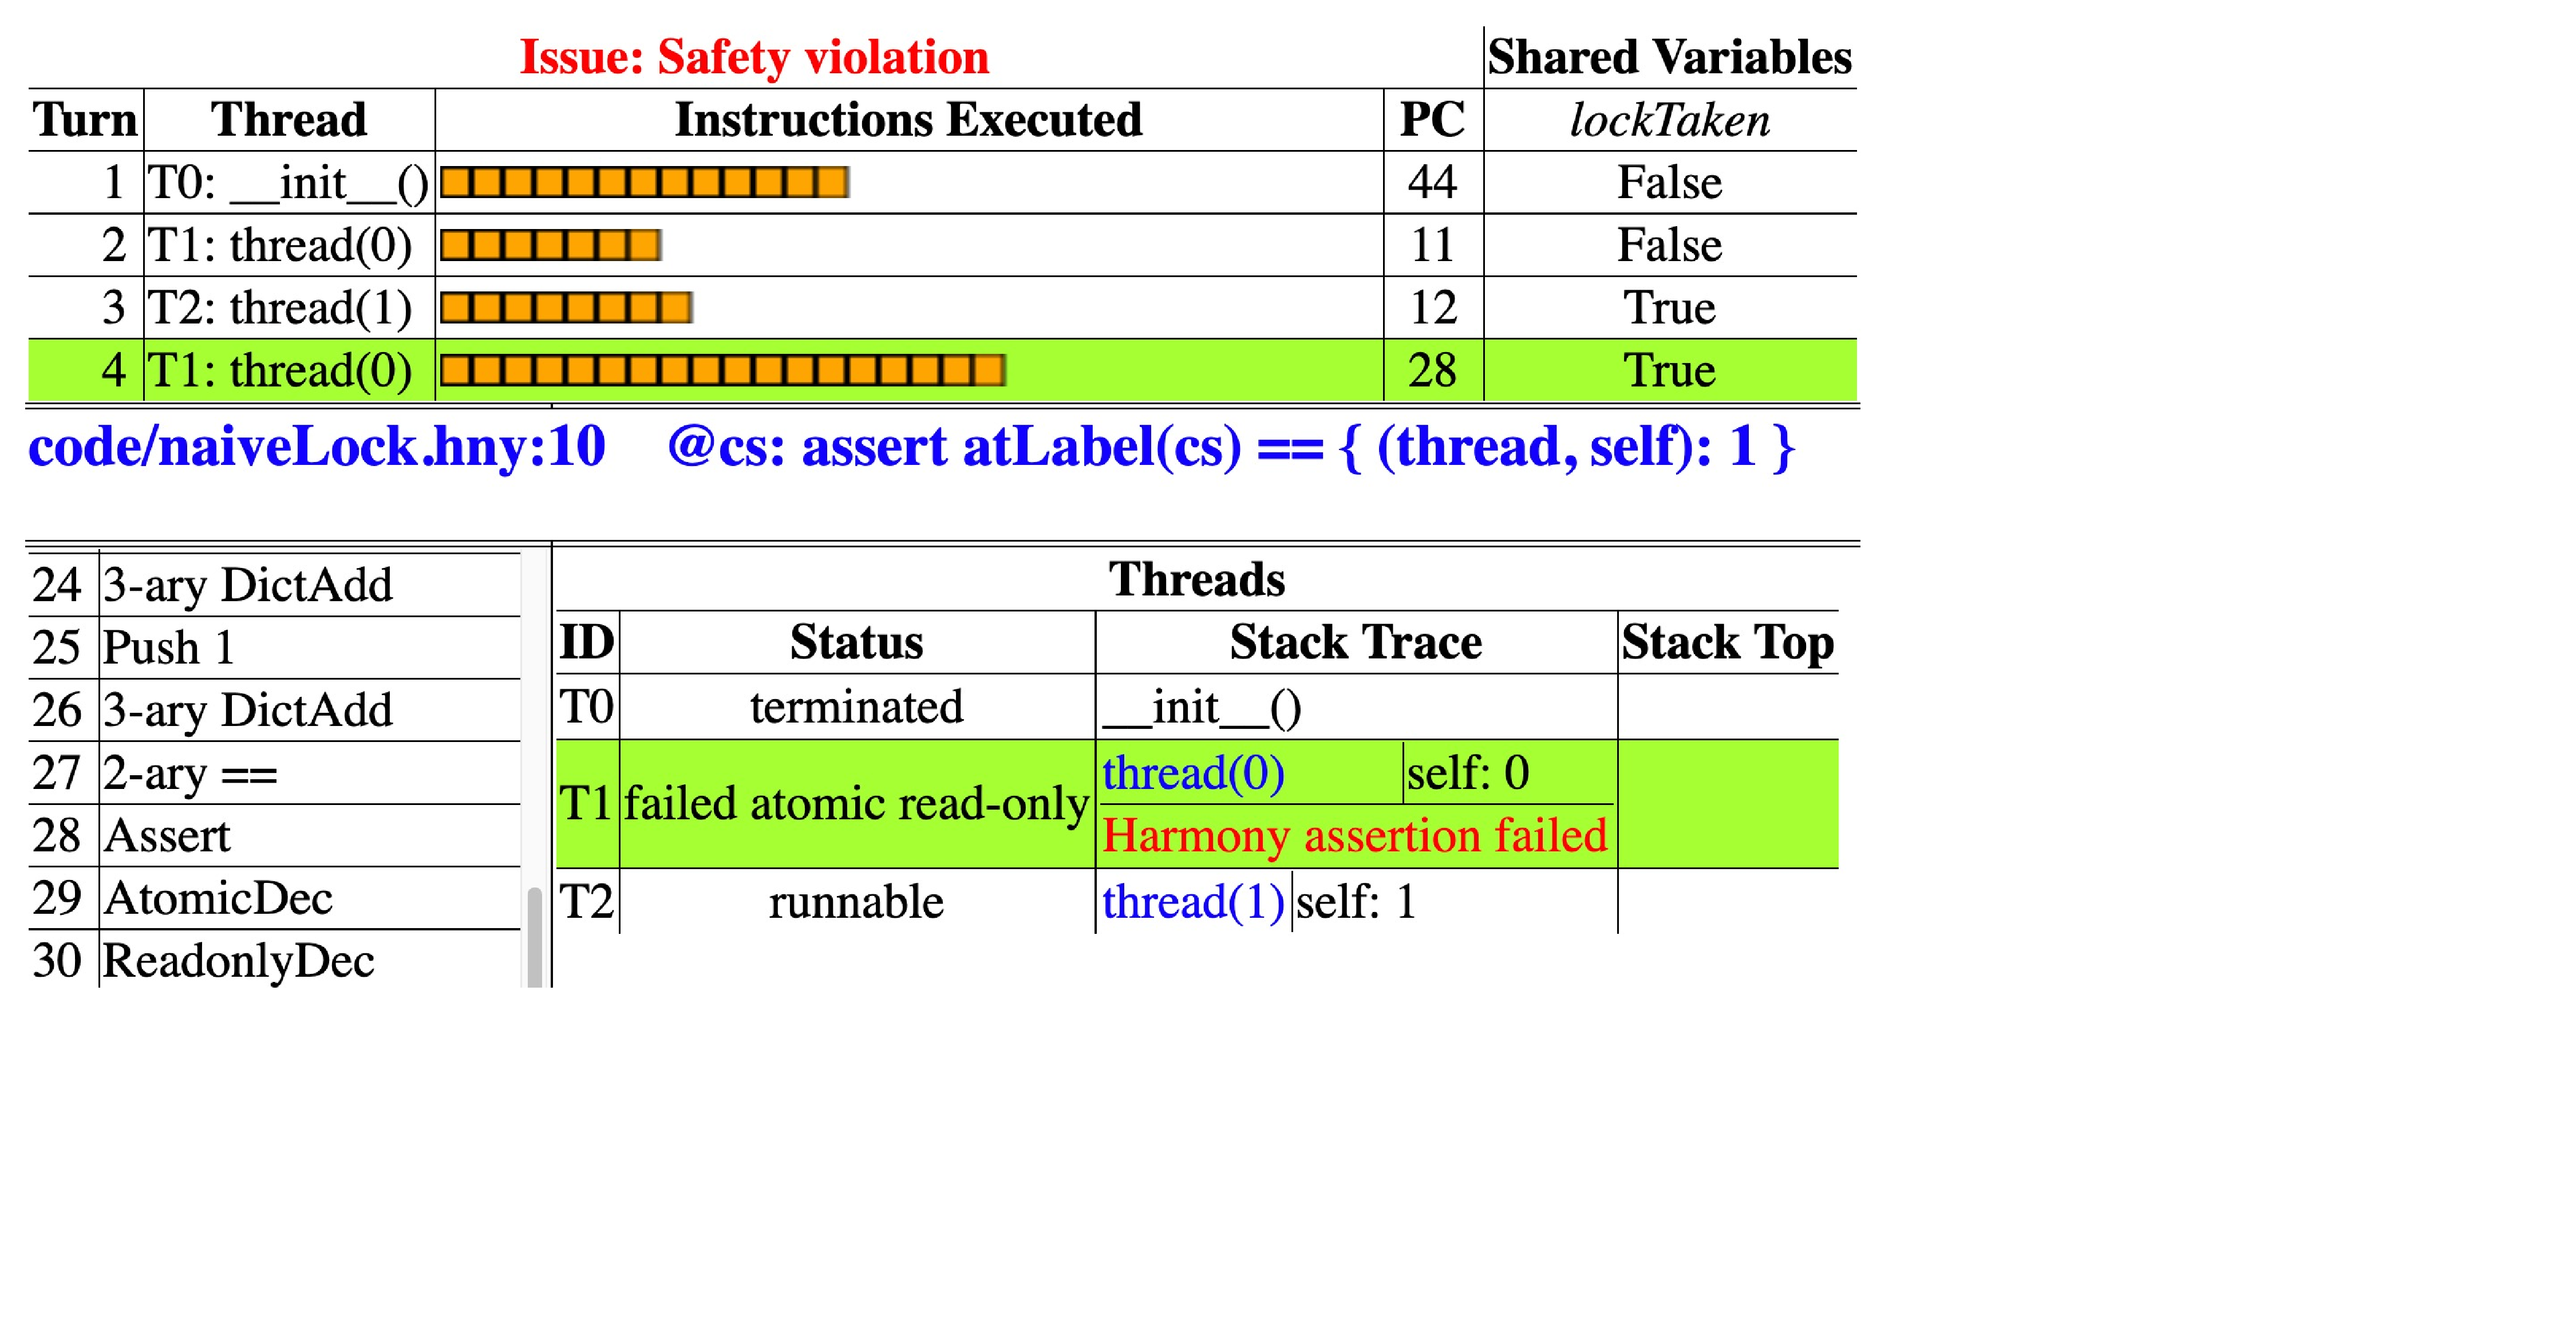
\includegraphics[width=0.8\textwidth]{figures/naiveLock.pdf}
\end{center}
\caption{The \harmonyref{naiveLock.html}{HTML output of running Harmony on \autoref{fig:naivelock}}.}
\label{fig:naiveLockhtml}
\end{figure}

\begin{figure}
\begin{code}
\harmonysource{naiveFlags}
\end{code}
\caption{\harmonylink{code/naiveFlags.hny} Na\"{\i}ve use of flags to solve mutual exclusion.}
\label{fig:naiveflags}
\end{figure}

\begin{figure}
\begin{center}
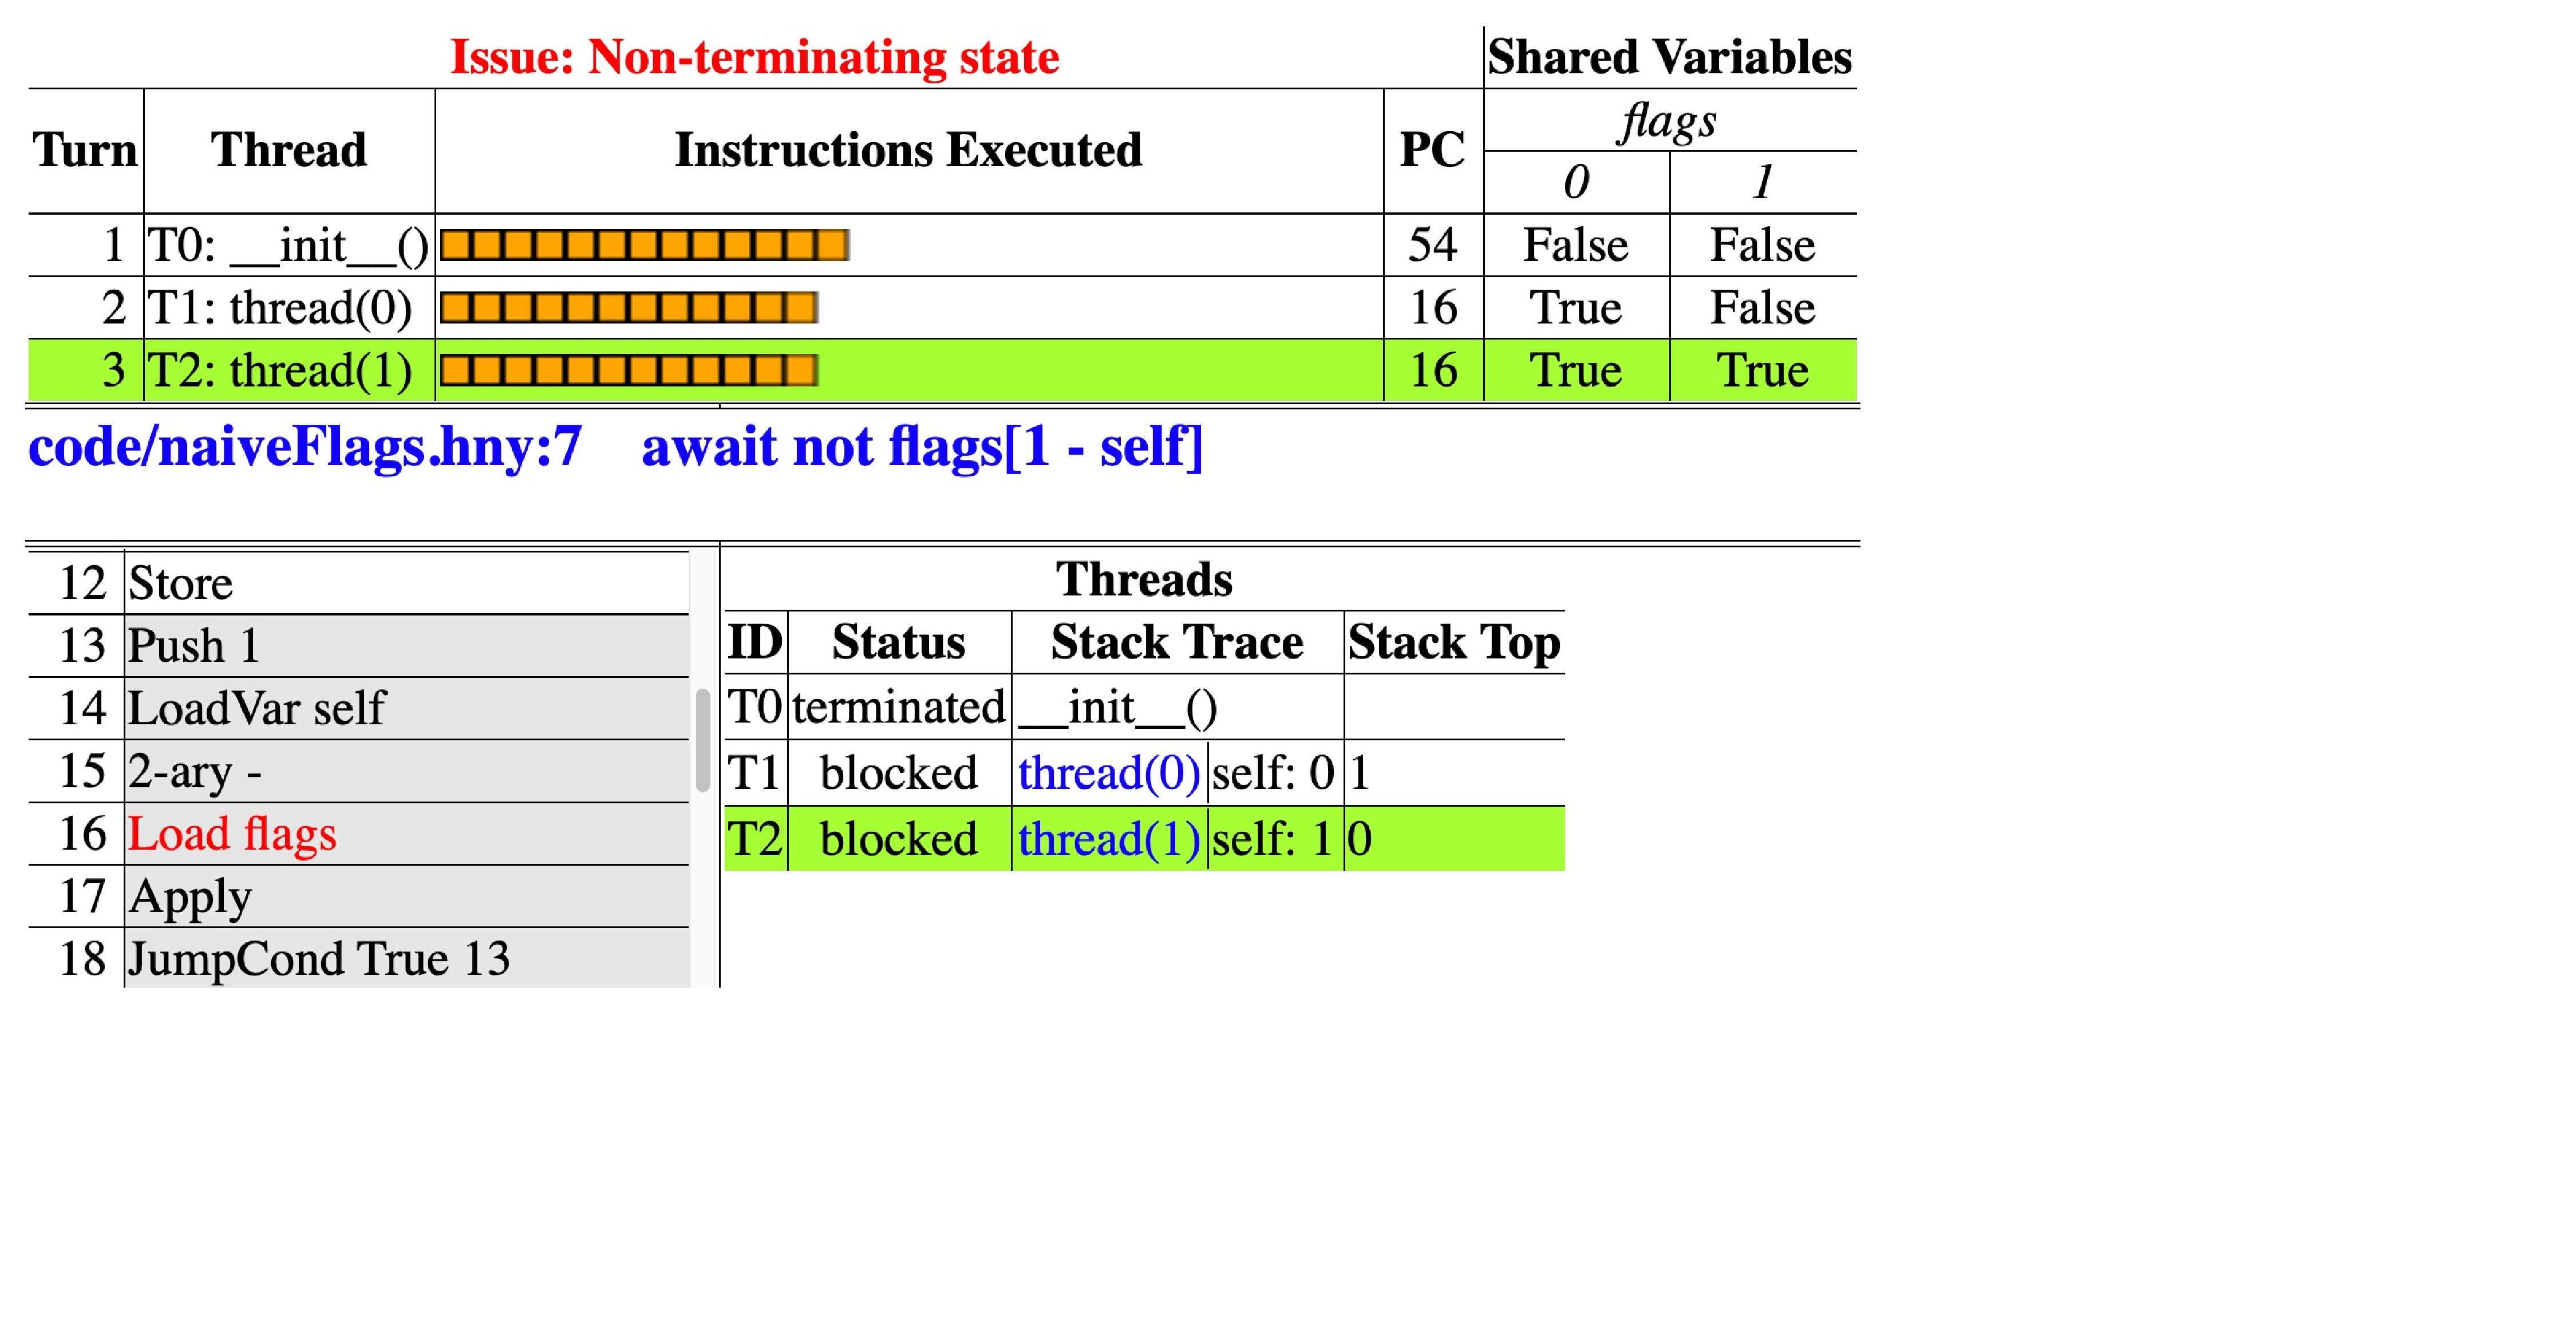
\includegraphics[width=0.8\textwidth]{figures/naiveFlags.pdf}
\end{center}
\caption{The \harmonyref{naiveFlags.html}{HTML output of running Harmony on \autoref{fig:naiveflags}}.}
\label{fig:naiveflagshtml}
\end{figure}

\begin{figure}
\begin{code}
\harmonysource{naiveTurn}
\end{code}
\caption{\harmonylink{code/naiveTurn.hny} Na\"{\i}ve use of turn variable to solve mutual exclusion.}
\label{fig:naiveturn}
\end{figure}

\glsadd{lock}%

You may already have heard of the concept of a \emph{lock}
\index{lock}%
and have realized that
it could be used to implement a critical section.
The idea is that the lock is like a baton that at most one thread can own
(or hold) at a time.
A thread that wants to enter the critical section at a time must obtain the
lock first and release it upon exiting the critical section.
% Note that the word ``lock'' does not describe the concept well---it really
% is more like a baton or token that only one thread can hold.

Using a lock is a good thought, but how does one implement one?
\autoref{fig:naivelock} presents a mutual exclusion attempt based on a
na\"{\i}ve (and, as it turns out, broken) implementation of a lock.
Initially the lock is not owned, indicated by \textit{lockTaken} being \texttt{False}.
To enter the critical section, a thread waits until \textit{lockTaken} is \texttt{False}
and then sets it to \texttt{True} to indicate that the lock has been taken.
The thread then executes the critical section.  Finally the thread
releases the lock by setting \textit{lockTaken} back to \texttt{False}.

Unfortunately, if we run the program through Harmony,
we find that the assertion still fails.
\autoref{fig:naiveLockhtml} shows the Harmony output.
Thread~0 finds that the lock is available, but just before it stores
\texttt{True} in \textit{lockTaken} in instruction~9, thread~1 gets
to run.
(Recall that you can hover your mouse over a machine instruction in order
to see what it does.)
Because \textit{lockTaken} is still \texttt{False}, it too
believes it can acquire the lock, and stores \texttt{True} in
\textit{lockTaken} and moves on to the critical section.
Finally, thread~0 moves on, also stores \texttt{True}
into \textit{lockTaken} and also moves
into the critical section.  Thread~0 is the one that detects the
problem.
The \textit{lockTaken} variable
suffers from the same sort of race condition as the \textit{count} variable
in \autoref{fig:inc}: testing and setting the lock
consists of several instructions.  It is thus possible
for both threads to believe the lock is available and to obtain the lock
at the same time.

Preventing multiple threads from updating the same variable,
\autoref{fig:naiveflags} presents a solution based on each thread having
a flag indicating that it is trying to enter the critical section.
A thread can write its own flag and read the flag of its peer.
After setting its flag, the thread waits until the other thread
($1 - \mathit{self}$) is not trying to enter the critical section.
If we run this program, the assertion does not fail.  In fact, this
solution does prevent both threads being in the critical section at
the same time.

To see why, first note the following invariant: if thread $i$ is in the
critical section, then \textit{flags}[$i$] == \texttt{True}.
Without loss of generality,
suppose that thread~0 sets \textit{flags}[0] at time $t_0$.
Thread 0 can only reach the critical section if at some time $t_1$,
$t_1 > t_0$, it finds that \textit{flags}[1] == \texttt{False}.
Because of the invariant, \textit{flags}[1] == \texttt{False} implies that
thread~1 is not in the critical section at time $t_1$.
Let $t_2$ be the time at which thread~0 sets \textit{flags}[0]
to \texttt{False}.  Thread~0 is in the critical section sometime
between $t_1$ and $t_2$.
It is easy to see that thread~1 cannot enter the critical section
between $t_1$ and $t_2$, because \textit{flags}[1] == \texttt{False} at
time $t_1$.  To reach the critical section between $t_1$ and $t_2$,
it would first have to set \textit{flags}[1] to \texttt{True} and
then wait until \textit{flags}[0] == \texttt{False}.  But that does not happen
until time $t_2$.

However, if you run the program through Harmony (\autoref{fig:naiveflagshtml}),
it turns out the solution
does have a problem: if both try to enter the critical section at the same
time, they may end up waiting for one another indefinitely.
(This is a form of \emph{deadlock}, which will be discussed in
\autoref{ch:deadlock}.)
Thus the
solution violates \emph{progress}.

The final na\"{\i}ve solution that we propose
is based on a variable called \textit{turn}.
Each thread politely lets the other thread have a turn first.
When \textit{turn} = $i$, thread~$i$ can
enter the critical section, while thread $1-i$ has to wait.
An invariant of this solution is that while thread~$i$ is in the critical
section, \textit{turn} == $i$.
Since \textit{turn} cannot be 0 and 1 at
the same time, mutual exclusion is satisfied.
The solution also has the nice property that the thread that has been waiting the
longest to enter the critical section can go next.

Run the program through Harmony.  It turns out that this solution also violates
\emph{progress}, albeit for a different reason:
if thread~$i$ terminates instead of entering the critical section,
thread $1-i$, politely, ends up waiting indefinitely for its turn.
Too bad, because it would have been a great solution if both
threads try to enter the critical section ad infinitum.

\section*{Exercises}
\begin{problems}
\item Run \autoref{fig:cs} using Harmony.  As there is no protection of the critical
section, mutual exclusion is violated,
the assertion should fail, and a trace should be reported.
Now insert
\begin{code}
\texttt{await False}
\end{code}
just before entering the critical section
in \autoref{fig:cs} and run Harmony again.
Mutual exclusion is guaranteed but progress is violated.
Harmony should print a trace
to a state from which a terminating state cannot be reached.
Describe in English the difference in the failure reports before
and after inserting the code.
\item See if you can come up with some different approaches that satisfy both
mutual exclusion and progress.  Try them with Harmony and see if they work or not.
If they don't, try to understand why.
If you get \emph{active busy waiting} or \emph{data race} reports, you probably
found a correct solution; you'll learn later how to suppress those.
Do not despair if you can't figure out how to develop a solution that satisfies both
mutual exclusion and progress---as we will find out, it is possible but not obvious.
\end{problems}

\chapter{Peterson's Algorithm}
\label{ch:peterson}
\index{Peterson's Algorithm}%

\begin{figure}
\begin{code}
\harmonysource{Peterson}
\end{code}
\caption{\harmonylink{code/Peterson.hny} Peterson's Algorithm}
\label{fig:peterson}
\end{figure}

\glsadd{sequential consistency}%
In 1981, Gary L.~Peterson came up with a beautiful solution to the mutual exclusion
problem, now known as ``Peterson's Algorithm''~\cite{Peterson81}.
The algorithm is an amalgam of the (incorrect) algorithms in
\autoref{fig:naiveflags} and \autoref{fig:naiveturn}, and is presented
in \autoref{fig:peterson}.
(The first line specifies that the \textit{flags} and \textit{turn}
variables should have \emph{sequential consistency}---it prevents
Harmony from complaining about data races involving these variables,
explained in \autoref{ch:spinlock}.)

A thread first indicates its interest in entering the critical section
by setting its flag.
It then politely gives way to the other thread should it also want to
enter the critical section---if both do so at the same time one will
win because writes to memory in Harmony are atomic.
The thread continues to be polite, waiting
until either the other thread is nowhere near the critical section
($\mathit{flag}[1 - \mathit{self}] == \mathtt{False}$) or has given way
($\mathit{turn} == \mathit{self}$).
Running the algorithm with Harmony shows that it satisfies both mutual
exclusion and progress.

\begin{figure}
\begin{center}
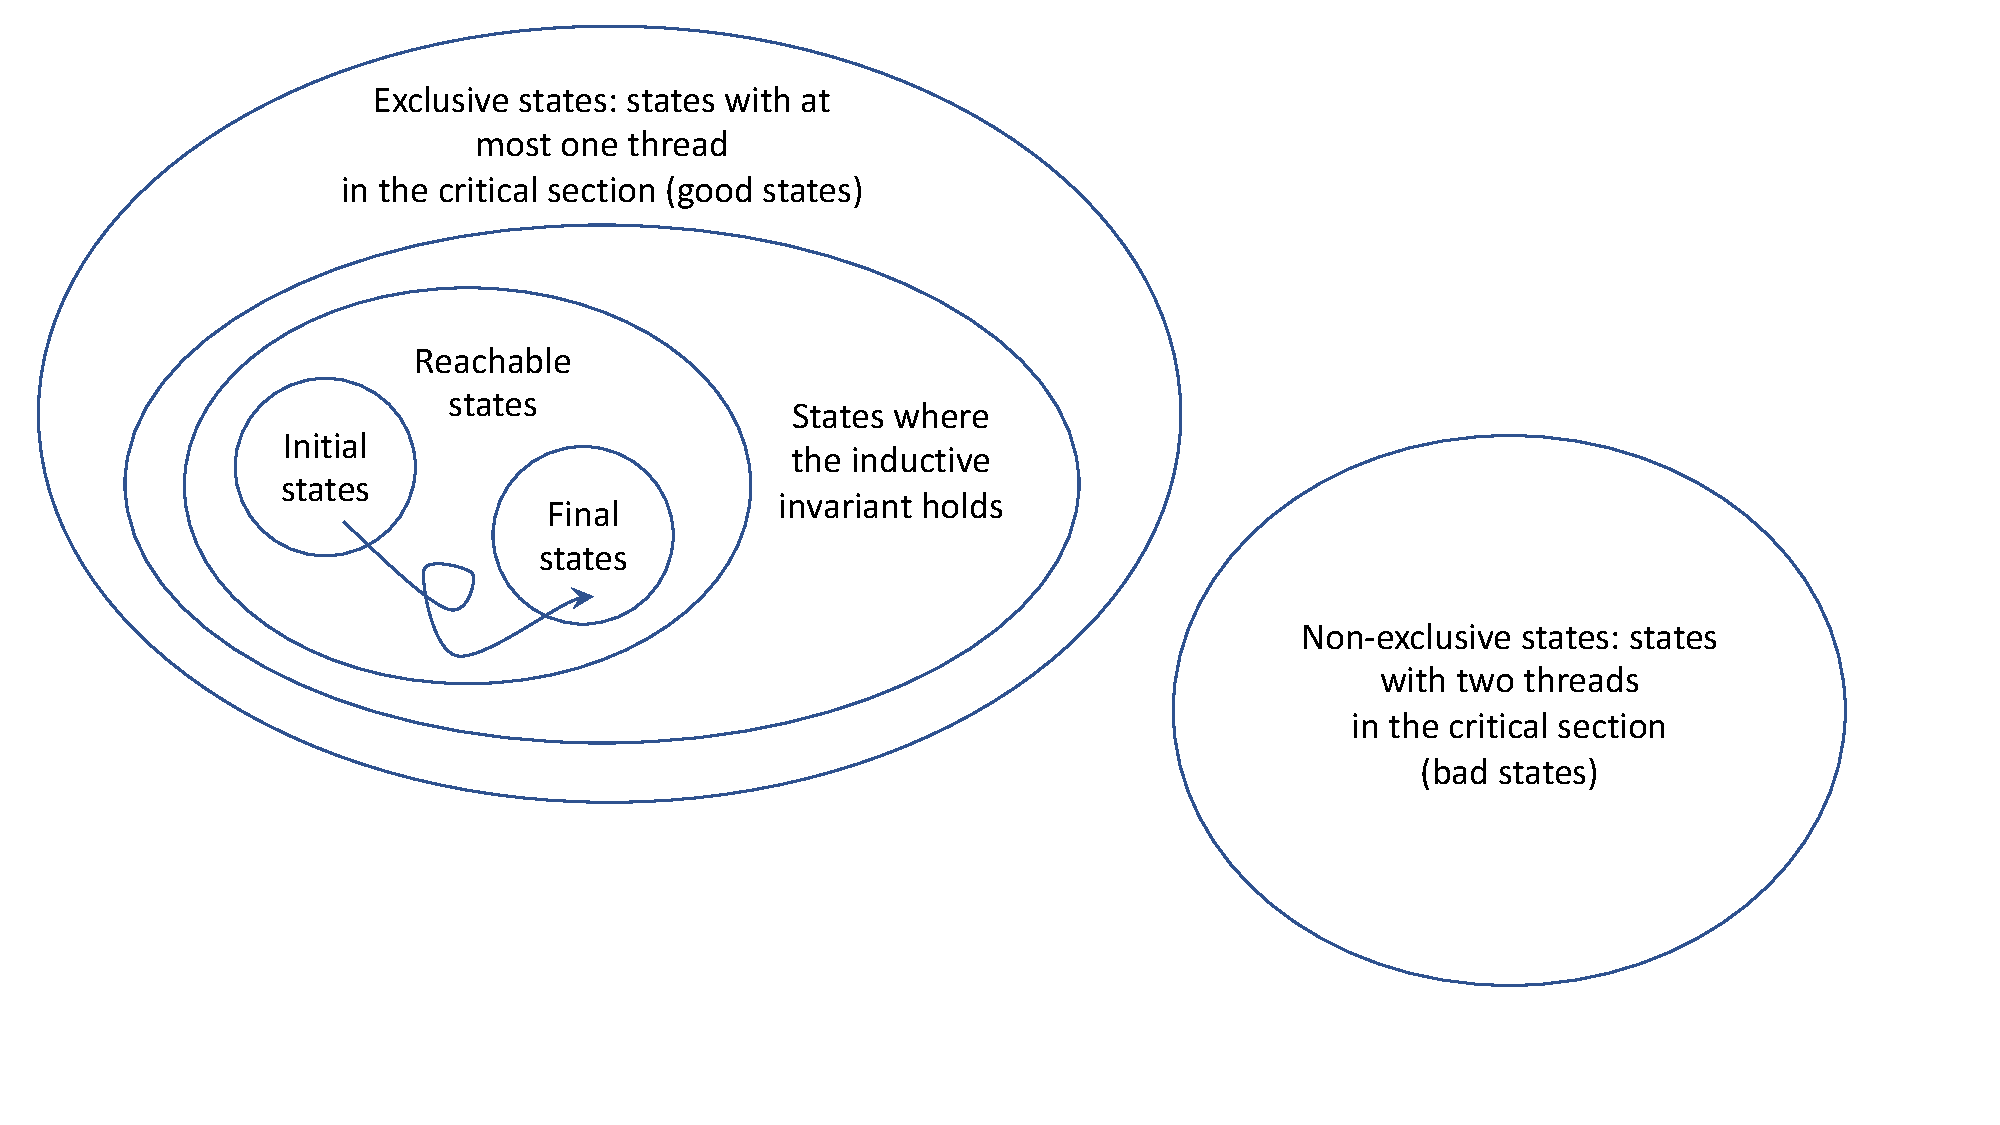
\includegraphics[width=6in]{figures/states-crop.pdf}
\end{center}
\caption{Venn diagram classifying all states and a trace.}
\label{fig:states}
\end{figure}

\glsadd{state}%
\glsadd{thread variable}%

Why does it work?  We will focus here on how one might go about proving
mutual exclusion for an algorithm such as Peterson's.
It turns out that doing so is not easy.
If you are interested in learning more about concurrent programming
but not necessarily in how to prove concurrent programs correct, you
may choose to skip the rest of this chapter.
If you are still here, you have to understand a little bit more about
how the Harmony virtual machine (HVM) works.
In \autoref{ch:harmonymachine} we talked about the concept of \emph{state}:
\index{state}%
at any point in time the HVM is in a specific state.
A state is comprised of the values of the shared variables as well as
the values of the thread variables
\index{thread variable}%
of each thread, including its
program counter and the contents of its stack.
Each time a thread executes a HVM machine instruction, the
state changes (if only because the program counter of the thread
changes).  We call that a \emph{step}.
\index{step}%
Steps in Harmony are atomic.

\glsadd{step}%
\glsadd{trace}%

The HVM starts in an initial state in which there is only
one thread and its program counter is~0.  A \emph{trace}
\index{trace}%
is a sequence of steps starting from the initial state.
When making a step, there are two sources of non-determinism
\index{non-determinism}%
in Harmony.
% \footnote{Actually, there is a third type called
% an \emph{interrupt}, discussed in \autoref{ch:interrupts}.}
One is when
there is more than one thread that can make a step.  The other is
when a thread executes a \texttt{choose} operation and there is
more than one choice.
Because there is non-determinism, there are multiple possible traces.
We call a state \emph{reachable}
\index{reachable state}%
if it is either the initial state
or it can be reached from the initial state through a finite trace.
A state is final
when there are no threads left to make state changes.

It is often useful to classify states.
\emph{Initial}, \emph{final}, and \emph{reachable}, and \emph{unreachable}
are all examples of classes of states.
\autoref{fig:states} depicts a Venn diagram of various classes of states
and a trace.
One way to classify states is to define a predicate over states.
All states in which $x$ = 1, or all states where
there are two or more threads executing, are examples of such predicates.
For our purposes, it is useful to define a predicate that says that at
most one thread is in the critical section.  We shall call such states
\emph{exclusive}.

An \emph{invariant} of a program
\index{invariant}%
is a predicate that holds over all states that are reachable by that program.
We want to show that exclusivity is an invariant because mutual exclusion means
that all reachable states are exclusive.
In other words, we want to show that the set of reachable states of executing
the program
is a subset of the set of states where there is at most one thread in the critical
section.

One way to prove that a predicate is an invariant is through induction
on the number of steps.  First you prove that the predicate holds over
the initial state.  Then you prove that for every reachable state,
and for every step from that reachable state, the predicate also holds
over the resulting state.
For this to work you would need a predicate that describes exactly which
states are reachable.
But we do not have such a predicate: we know how to define the set
of reachable states inductively, but given an arbitrary state it is not
easy to see whether it is reachable or not.

To solve this problem, we will use what is called an
\emph{inductive invariant}.
\index{inductive invariant}%
An inductive invariant~$\mathcal{I}$ is a predicate over states that satisfies the following:
\begin{itemize}
\item $\mathcal{I}$ holds in the initial state.
\item For any state in which $\mathcal{I}$ holds (including unreachable ones) and for any
thread in the state, if the thread takes a step, then $\mathcal{I}$ also holds in the
resulting state.
\end{itemize}

One candidate for such a predicate is exclusivity itself.
After all, it certainly holds over the initial state.
And as Harmony has already determined, exclusivity is an invariant:
it holds over every reachable state.
Unfortunately, exclusivity is not an \emph{inductive} invariant.
To see why, consider the following state $s$: let thread~0 be at label \texttt{@cs}
and thread~1 be at the start of the \textbf{await} statement.
Also, in state $s$, $\mathit{turn} = 1$.  Now let
thread~1 make a step.  Because $\mathit{turn} = 1$,
thread~1 will stop waiting and also enter the critical
section, entering a state that is not exclusive.
So, exclusivity is an invariant (holds over every reachable state, as demonstrated
by Harmony),
but not an inductive invariant.
It will turn out that $s$ is not reachable.

We are looking for an inductive invariant that \emph{implies} exclusivity.
In other words, the set of states where the inductive invariant holds
must be a subset of the set of states where there is at most one thread in
the critical section.

Let us begin with considering the following important property:
$\mathcal{F}(i) = \mathtt{thread}(i)@[8 \cdots 15] \Rightarrow \mathit{flags}[i]$,
that is, if thread~$i$ is executing in lines 8 through 15, then $\mathit{flags}[i]$
is set.
Although it does not, by itself, imply exclusivity, we can show that
$\mathcal{F}(i)$ is an inductive invariant (for both threads~0 and~1).
To wit, it holds in the initial state, because in the initial state thread $i$ does
not even exist yet.
Now we have to show that if $\mathcal{F}(i)$ holds in some state, then
$\mathcal{F}(i)$ also holds in a next state.
Since only thread~$i$ ever changes $\mathit{flags}[i]$, we only need to
consider steps by thread~$i$.
Since $\mathcal{F}(i)$ holds, there are two cases to consider:
\begin{enumerate}
\item states in which $\mathit{flags}[i] = \texttt{true}$
\item states in which $\lnot \mathtt{thread}(i)@[8 \cdots 15]$
(because false implies anything)
\end{enumerate}
In each case we need to show that if thread $i$ takes a step, 
$\mathcal{F}(i)$ still holds.
In the first case, there is only one step that thread $i$ can take that would
set $\mathit{flags}[i]$ to false: the step in line 15.  But executing the line
would also take the thread out of lines $8 \cdots 15$, so $\mathcal{F}(i)$ continues to hold.
In the second case (thread $i$ is not executing in lines $8 \cdots 15$), the only step
that would cause thread $i$ to execute in lines $8 \cdots 15$ would be the step in line 7.
But in that case $\mathit{flags}[i]$ would end up being true, so
$\mathcal{F}(i)$ continues to hold as well.
So, $\mathcal{F}(i)$ is an inductive invariant (for both threads~0 and~1).

While $\mathcal{F}(i)$ does not imply mutual exclusion, it does imply the following useful
invariant: $\mathtt{thread}(i)@cs \Rightarrow \mathit{flags}[i]$: when thread $i$ is
at the critical section, $\mathit{flags}[i]$ is set.  This seems obvious from the code,
but now you know how to prove it.

We need a stronger inductive invariant than $\mathcal{F}(i)$ to prove mutual exclusion.
What else do we know when thread $i$ is in the critical section?
Let $\mathcal{C}(i) = \lnot\mathit{flags}[1 - i] \lor \mathit{turn} = i$, that is,
the condition on the \textbf{await} statement for thread~$i$.
In a sequential program, $\mathcal{C}(i)$ would clearly hold if thread $i$ is in
the critical section: $\mathtt{thread}(i)@cs \Rightarrow \mathcal{C}(i)$.
However, because thread $1-i$ is executing concurrently, this property does not
hold.  In particular, suppose thread 0 is at the critical section, $\mathit{flags}[0]$ = true,
$\mathit{turn} = 1$, and thread 1 just finished the step in line 7,
setting $\mathit{flags}[1]$ to true.  Notice that $C(0)$ is now violated.

\begin{figure}
\begin{code}
\harmonysource{PetersonInductive}
\end{code}
\caption{\harmonylink{code/PetersonInductive.hny} Peterson's Algorithm with Inductive Invariant}
\label{fig:petersonproof}
\end{figure}

Instead, we will use the following property: $\mathcal{G}(i) =
\mathtt{thread}(i)@\mathtt{cs} \Rightarrow \mathcal{C}(i) \lor \mathtt{thread}(1-i)@\mathtt{gate}$.
That is, if thread $i$ is at the critical section, then
either $\mathcal{C}(i)$ holds or thread $1-i$ is about to execute line 8.
\autoref{fig:petersonproof} formalizes $\mathcal{G}(i)$ in Harmony.
The label \texttt{@gate} refers to the step that sets \textit{turn} to $1-i$.
You can run \autoref{fig:petersonproof} to determine
that $\mathcal{G}(i)$ is an invariant for $i = 0, 1$.
Moreover, if $\mathcal{F}(i)$ and $\mathcal{G}(i)$ both hold for $i = 0, 1$,
then mutual exclusion holds.  We can show this using proof by
contradiction.  Suppose mutual exclusion is violated and thus both threads are in
the critical section.  By $\mathcal{F}$ it must be the case that both
\textit{flags} are true.  By $\mathcal{G}$ and the fact that neither thread
is at label \texttt{@gate}, we know that both $C(0)$ and $C(1)$ must hold.
This then implies that $\mathit{turn} = 0 \land \mathit{turn} = 1$, providing
the desired contradiction.

We claim that $\mathcal{G}(i)$ is an inductive invariant.
First, since neither thread in in the critical section in the initial state,
it is clear that $\mathcal{G}(i)$ holds in the initial state.
Without loss of generality, suppose $i=0$ (a benefit from the fact that the algorithm is
symmetric for both threads).  We still have to show that if we are in a state
in which $\mathcal{G}(0)$ holds, then any step will result in a
state in which $\mathcal{G}(0)$ still holds.

First consider the case that thread~0 is at label \texttt{@cs}.  If thread~0
were to take a step, then in the next state thread~0 would be no longer
at that label and $\mathcal{G}(0)$ would hold trivially over the next state.
Therefore we only need to consider a step by thread~1.
%
From $\mathcal{G}$ we know that one of the following three cases must hold before
thread~1 takes a step:
\begin{enumerate}
\item \textit{flags}[1] = \texttt{False};
\item \textit{turn} = 0;
\item thread~1 is at label \texttt{@gate}.
\end{enumerate}

Let us consider each of these cases.
We have to show that if thread~1 takes a step, then one of those
cases must hold after the step.
In the first case, if thread~1 takes a step, there are two possibilities:
either $flags[1]$ will still be \texttt{False} (in which case the first case
continues to hold), or $flags[1]$ will be \texttt{True}
and thread~1 will be at label \texttt{@gate} (in which case the third case
will hold).
We know that thread~1 never sets \textit{turn} to 1, so
if the second case holds before the step, it will also hold after the step.
Finally, if thread~1 is at label \texttt{@gate} before the step, then after
the step \textit{turn} will equal 0, and therefore the second case will hold
after the step.

Now consider the case where thread~0 is not in the critical section,
and therefore $\mathcal{G}(0)$ holds trivially because false implies
anything.
There are three cases to consider:
\begin{enumerate}
\item Thread~1 takes a step.  But then thread~0 is still not in the critical
section and $\mathcal{G}(0)$ continues to hold;
\item Thread~0 takes a step but still is not in the critical section.
Then again $\mathcal{G}(0)$ continues to hold.
\item Thread~0 takes a step and ends up in the critical section.
Because thread~0 entered the critical section, we know that
\textit{flags}[1] = \texttt{False} or \textit{turn} == 0 because
of the \texttt{await} condition.
And hence $\mathcal{G}(0)$ continues to hold in that case as well.
\end{enumerate}

We have now demonstrated mutual exclusion in Peterson's Algorithm in two
different ways: one by letting Harmony explore all possible executions, the
other using inductive invariants and proof by induction.  The former
is certainly easier, but it does not provide intuition for why the
algorithm works.  The second provides much more insight.

Even though they are not strictly necessary, we encourage you
to include invariants in your Harmony code.
They can provide important insights into why the code works.

A cool anecdote is the following.  When the author of Harmony had to teach
Peterson's Algorithm, he refreshed his memory by looking at the Wikipedia
page.  The page claimed that the following predicate is invariant:
if thread $i$ is in the critical section, then $\mathcal{C}(i)$ (i.e.,
$\mathcal{G}$ without the disjunct that thread $1-i$ is at label \texttt{@gate}).
To demonstrate that this predicate is not invariant, you can remove the
disjunct from \autoref{fig:petersonproof} and run it to get a
counterexample.

This anecdote suggests the following.  If you need to do a proof by induction
of an algorithm, you have to come up with an inductive invariant.
Before trying to prove the algorithm, you can check that the predicate is
at least invariant by testing it using Harmony.  Doing so could potentially
avoid wasting your time on a proof that will not work because the
predicate is not invariant, and therefore not an inductive invariant either.
(The author fixed the Wikipedia page with the help of Fred B.~Schneider.)

\section*{Exercises}
\begin{problems}
\item \autoref{fig:csonebit} presents another solution to the
mutual exclusion problem.  It is similar to the one in
\autoref{fig:naiveflags}, but has a thread \emph{back out and try again}
if it finds that the other thread is either trying to enter the critical
section or already has.  Compare this algorithm with Peterson's.
Why does Harmony complain about \emph{active busy waiting}?
\item
Can you find one or more inductive invariants for the algorithm in
\autoref{fig:csonebit} to prove it correct?
Here's a pseudo-code version of the algorithm to help you.  Each line
is an atomic action:
\begin{code}
\begin{verbatim}
    initially: flagX = flagY = False

    thread X:                          thread Y:
        X0: flagX = True                   Y0: flagY = True
        X1: if not flagY goto X4           Y1: if not flagX goto Y4
        X2: flagX = False                  Y2: flagY = False
        X3: goto X0                        Y3: goto Y0
        X4: ...critical section...         Y4: ...critical section...
        X5: flagX = False                  Y5: flagY = False
\end{verbatim}
\end{code}
\item \label{ex:reorder}
A colleague of the author asked if the first two assignments in
Peterson's algorithm (setting \textit{flags}[\textit{self}])
to \texttt{True} and \textit{turn} to $1 - \mathit{self}$) can be reversed.
After all, they are different variables assigned independent values---in a
sequential program one could surely swap the two assignments.
See if you can figure out for yourself if the two assignments can be
reversed.  Then run the program in \autoref{fig:peterson} after reversing
the two assignments and describe in English what happens.
\item Bonus question:
Can you generalize Peterson's algorithm to more than two threads?
\item Bonus question:
Implement
\href{https://en.wikipedia.org/wiki/Dekker%27s_algorithm}{Dekker's Algorithm},
\href{https://en.wikipedia.org/wiki/Eisenberg_%26_McGuire_algorithm}{Eisenstein and McGuire's Algorithm},
\href{https://en.wikipedia.org/wiki/Szymanski%27s_algorithm}{Szymański's Algorithm}, or the
\href{https://en.wikipedia.org/wiki/Lamport%27s_bakery_algorithm}{Lamport's Bakery Algorithm}.
Note that the last one uses unbounded state, so you should modify the threads so they
only try to enter the critical section a bounded number of times.
\end{problems}

\begin{figure}
\begin{code}
\harmonysource{csonebit}
\end{code}
\caption{\harmonylink{code/csonebit.hny} Mutual exclusion using a flag per thread.}
\label{fig:csonebit}
\end{figure}

\chapter{Harmony Methods and Pointers}
\label{ch:method}
\index{Harmony method}%

A method \texttt{m} with argument $a$ is invoked in its
most basic form as follows (assigning the result to~\texttt{r}).
\begin{code}
$r$ = m $a$;
\end{code}
That's right, no parentheses are required.  In fact, if you invoke
\texttt{m}($a$), the argument is ($a$), which is the same
as $a$.
If you invoke \texttt{m()}, the argument is \texttt{()},
which is the empty tuple.
If you invoke \texttt{m}($a$, $b$), the argument is ($a$, $b$),
the tuple consisting of values $a$ and $b$.

You may note that all this looks familiar.  Indeed, the syntax
is the same as that for dictionaries (see \autoref{ch:harmonymachine}).
Both dictionaries and methods map Harmony values to Harmony values,
and their syntax is indistinguishable.
If \texttt{f} is either a method or a
dictionary, and $x$ is an arbitrary Harmony value, then
\texttt{f} $x$, \texttt{f}($x$), and \texttt{f}[$x$] are all
the same expression in Harmony.

\begin{figure}
\begin{code}
\harmonysource{PetersonMethod}
\end{code}
\caption{\harmonylink{code/PetersonMethod.hny} Peterson's Algorithm accessed through methods.}
\label{fig:petersonmethods}
\end{figure}

Harmony does not have a \textbf{return} statement.  (You can assign a return value
to a method by setting the \textit{result} variable.)  Neither does it support
\textbf{break} or \textbf{continue} statements in loops.  One reason for their absence is
that, particularly in concurrent programming, such control flow directions are highly
error-prone.  It's too easy to forget to, say, release a lock when returning a value in the
middle of a method, a major source of bugs in practice.

Harmony is not an object-oriented language like Python is.  In Python
you can pass a reference to an object to a method, and that method
can then update the object.  In Harmony, it is also sometimes convenient
to have a method update a shared variable specified as an argument.
For this, as mentioned in \autoref{ch:harmonymachine},
each shared variable has an \emph{address}, itself a Harmony value.
\index{address}%
If $x$ is a shared variable, then the expression ?$x$ is the address of $x$.
If a variable contains an address, we call that variable a \emph{pointer}.
\index{pointer}%
If $p$ is a pointer to a shared variable, then the
expression \texttt{!}$p$ is the value of the shared variable.
In particular, \texttt{!?}$x$ == $x$.
This is similar to how C pointers work (\texttt{*\string&}$x$ == $x$).

Often, pointers point to dictionaries, and so if $p$ is such a pointer,
then $(!p).\mathtt{field}$ would evaluate to the specified field in the dictionary.
Note that the parentheses in this expression
are needed, as \texttt{!}\textit{p}\texttt{.field} would wrongly evaluate
\texttt{!}(\textit{p}\texttt{.field}).
$(!p).\mathtt{field}$ is such a common expression that, like C, Harmony supports the
shorthand $p-$$>$\texttt{field}, which greatly improves readability.

\autoref{fig:petersonmethods} again shows Peterson's algorithm,
but this time with methods defined to enter and exit the critical
section.
The name \textit{mutex} is often used to denote a variable or value
that is used for mutual exclusion.
\texttt{P\_mutex} is a method that returns a ``mutex,'' which, in this
case, is a dictionary that contains Peterson's Algorithm's shared memory state:
a turn variable and two flags.
Both methods \texttt{P\_enter} and \texttt{P\_exit} take two arguments:
a pointer to a mutex and the thread identifier (0 or 1).
$\mathit{pm}$$\rightarrow$$\mathtt{turn}$ is the value of the \texttt{.turn} key
in the dictionary that \textit{pm} points to. 

You can put the first three methods in its own Harmony source file
and include it using the Harmony \texttt{import} statement.
\index{import statement}%
\index{module}%
This would make the code usable by multiple applications.

Finally, methods can have local variables.
Different from Python, Harmony local variables must be
explicitly bound within a scope.
You have already seen examples: the arguments to the method,
the variable \textit{result}, and the bound variable (or
variables) within a \texttt{for} statement.
The \texttt{let} statement allows declaring additional
local variables.  For example:
\texttt{let} $x = 3$: $y$ $+$$=$ $x$ adds 3 to the global variable
$y$.
See \autoref{sec:vars} for more information.

\begin{figure}
\begin{code}
\harmonysource{clock}
\end{code}
\caption{\harmonylink{code/clock.hny} Harmony program that finds page replacement anomalies.}
\label{fig:clock}
\end{figure}

If you are ready to learn about how locks are implemented in practice,
you can now skip the rest of this chapter.  But if you would like to
see a cool example of using the concepts introduced in this chapter,
hang on for a sequential Harmony program that finds anomalies in page
replacement algorithms.
In 1969, B\'{e}l\'{a}ady et al. published a paper~\cite{Belady69}
that showed that making a
cache larger does not necessarily lead to a higher hit ratio.  He showed
this for a scenario using a FIFO replacement policy when the cache is full. 
The program in \autoref{fig:clock} will find exactly the same scenario
if you define \texttt{FIFO} to be \textbf{True}.  Moreover, if you define
\texttt{FIFO} to be \textbf{False}, it will find a scenario for the
CLOCK replacement policy~\cite{clock}, often used in modern operating systems.

In this program, \texttt{CLOCK} maintains the state of a cache
(in practice, typically pages in memory).
The set \texttt{recent} maintains whether an access to the cache
for a particular reference was recent or not.
(It is not used if \texttt{FIFO} is \textbf{True}.)
The integer \texttt{misses} maintains the number of cache misses.
Method \texttt{ref}(\textit{ck}, $x$) is invoked when $x$ is
referenced and checked against the cache \textit{ck}.

The program declares two caches: one with 3 entries (\textit{clock3})
and one with 4 entries (\textit{clock4}).
The interesting part is in the last block of code.
It runs every sequence of references of up to 100 entries, using
references in the range 1 through 5.
Note that all the constants chosen in this program (3, 4, 5, 100)
are the result of some experimentation---you can try other ones.
To reduce the search space, the first four references are pinned
to 1, 2, 3, and 4.
Further reducing the search space, the program never repeats the
same reference twice in a row (using the local variable \texttt{last}).

The two things to note here is the use of the \textbf{choose}
expression and the \textbf{assert} statement.  Using \texttt{choose}
we are able to express searching through all possible strings of
references without a complicated nested iteration.
Using \texttt{assert} we are able to express the anomaly we are
looking for.

In case you want to check if you get the right results.  For \texttt{FIFO},
the program finds (in a few minutes) the same anomaly that
B\'{e}l\'{a}dy et al. found: 1 2 3 4 1 2 5 1 2 3 4 5.
For the \texttt{CLOCK} algorithm the program actually finds a shorter
reference string: 1 2 3 4 2 1 2 5 1 2.

\chapter{Spinlock}
\label{ch:spinlock}
\index{spinlock}%

\glsadd{spinlock}%

\begin{figure}
\begin{code}
\harmonysource{spinlock}
\end{code}
\caption{\harmonylink{code/spinlock.hny} Mutual Exclusion using a ``spinlock'' based on test-and-set.}
\label{fig:tas}
\end{figure}

\autoref{fig:naivelock} showed a faulty attempt at solving mutual
exclusion using a lock.  The problem with the implementation of the
lock is that checking the lock and setting it if it is available is
not \emph{atomic}.  Thus multiple threads contending for the lock
can all ``grab the lock'' at the same time.  While Peterson's
algorithm gets around the problem, it is not efficient, especially
if generalized to multiple threads.
Worse, Peterson relies on load and store operations to be executed
atomically, but this may not be the case.
There are a variety of possible reasons for this.

\begin{itemize}
\item Variables may have more bits than the processor's data bus.
For example, variables may have 32 bits, but the data bus may only
have 16 bits.  Thus to store or load a variable takes two 16-bit
operations each.  Take, for example, a variable that has value
0xFFFFFFFF, and consider a concurrent load and store operation on
the variable.
The store operation wants to clear the variable, but because it
takes two store operations on the bus, the load operation may
return either 0xFFFF0000 or 0x0000FFFF, a value that the variable
never was supposed to have.
This is the case even if the processor supports a 32-bit load or
store machine instruction: on the data bus it is still two
operations.
\item Modern processors sometimes re-orders load and store operations
(out-of-order execution) for improved performance.  On a sequential processor,
the re-ordering is not a problem as the processor only re-orders
operations on independent memory locations.  However, as \autoref{ex:reorder}
showed, Peterson's algorithm breaks down if operations are re-ordered.
Some memory caches can also cause non-atomic behavior of memory when shared
among multiple cores.
\item Even compilers, in their code generation, may make optimizations
that can reorder operations, or even eliminate operations, on variables.
For example, a compiler may decide that it is unnecessary to read the same
variable more than once, because how could it possibly change if there
are no store operations?
\end{itemize}

Peterson's algorithm relies on a \emph{sequential consistent memory model}
and hence the \textbf{sequential} statement: without it Harmony will
complain about data races.
More precisely, the \textbf{sequential} statement says that the
program relies on memory load and store instructions operating on
the indicated variables to be performed sequentially, and that this
order should be consistent with the order of operations invoked on each
thread.
The default memory models of C and Java are not sequentially
consistent.
The unfortunately named \texttt{volatile} keyword in Java has
a similar function as Harmony's \texttt{sequential} keyword.
Like many constructions in Java, its \texttt{volatile} keyword
was borrowed from C and C++.
However, in C and C++ they do \emph{not} provide sequential
consistency, and one cannot implement Peterson's algorithm in
C or C++ directly.

\glsadd{atomic instruction}%
For proper synchronization, multi-core processors provide so-called
\emph{atomic instructions}: \index{atomic instruction}%
special machine instructions
that can read memory and then write it in an indivisible step.
%
While the HVM does not have any specific built-in atomic instructions
besides loading and storing variables,
it does have support for executing multiple instructions atomically.
This feature is available in the Harmony language in two ways.
First, any Harmony statement can be made atomic by placing a label in front
of it.  Second, a group of Harmony statements can be made atomic
through the \textbf{atomic}
\index{atomic statement}%
statement.
We can use \textbf{atomic} statement blocks to implement a wide variety of
atomic operations.
For example, we could fix the program in \autoref{fig:inc} by
constructing an atomic increment operation for a counter, like so:
\begin{code}
\harmonysource{atomicinc}
\end{code}

To support implementing locks,
many CPUs have an atomic ``test-and-set'' (TAS)
\index{test-and-set}%
\index{TAS}%
operation.
Method \texttt{tas} in \autoref{fig:tas} shows its specification.
Here $s$ points to a shared Boolean variable and $p$
to a private Boolean variable, belonging to some thread.
The operation copies the value of the shared variable to the
private variable (the ``test'')
and then sets the shared variable to \texttt{True} (``set'').

\autoref{fig:tas} goes on to implement mutual exclusion for
a set of \texttt{N} threads.
The approach is called \emph{spinlock},
\index{spinlock}%
because each thread is ``spinning'' (executing a tight loop) until
it can acquire the lock.
The program uses $\mathtt{N}+1$ variables.
Variable \textit{shared} is initialized to \texttt{False} while
\textit{private}[$i$] for each thread $i$ is initialized to \texttt{True}.

An important invariant, $\mathcal{I}_1$, of the program is that at any time at most
one of these variables is \texttt{False}.
Another invariant, $\mathcal{I}_2(i)$, is that if thread $i$ is executing between
lines $18 \cdots 22$ (which includes the critical section),
then \textit{private}[$i$] == \texttt{False}.
Between the two (i.e., $\mathcal{I}_1 \land \forall i: \mathcal{I}_2(i)$),
it is clear that only one thread can be in the
critical section at the same time.
For those who read through the previous chapter:
$\mathcal{I}_1 \land \forall i: \mathcal{I}_2(i)$ is an inductive invariant.

To see that invariant $\mathcal{I}_1$ is maintained, note that
\texttt{!}$p$ == \texttt{True} upon entry of \texttt{tas}
(because of the condition on the \textbf{while} loop that the
\texttt{tas} method is invoked in).
There are two cases:
\begin{enumerate}
\item \texttt{!}$s$ is \texttt{False} upon entry to \texttt{tas}.
Then upon exit \texttt{!}$p$ == \texttt{False} and \texttt{!}$s$ == \texttt{True},
maintaining the invariant.
\item \texttt{!}$s$ is \texttt{True} upon entry to \texttt{tas}.
Then upon exit nothing has changed, maintaining the invariant.
\end{enumerate}
Invariant $\mathcal{I}_1$ is also easy to verify for exiting the critical section
because we can assume, by the induction hypothesis, that $\textit{private}[i]$ is
\texttt{True} just before exiting the critical section.
Invariant $\mathcal{I}_2(i)$ is obvious as (i) thread $i$ only proceeds to the critical
section if \textit{private}[$i$] is \texttt{False}, and (ii) no other thread modifies
\textit{private}[$i$].

Harmony can check these invariants as well.
$\mathcal{I}_2(i)$ is checked by the \textbf{assert} statement.
But how would one go about checking an
invariant like $\mathcal{I}_1$?  Invariants must hold for every state.
For $\mathcal{I}_2$ we only need an assertion at label \texttt{@cs} because the
premise is that there is a thread at that label.  However, we would
like to check $\mathcal{I}_1$ in \emph{every state} (after the variables have
been initialized).
Harmony supports checking such invariants using the \texttt{invariant}
keyword.
The expression counts the number of \texttt{False} values and checks that
the result is less than or equal to 1.
Harmony checks the expression in every reachable state.

\section*{Exercises}
\begin{problems}
\item Implement an atomic swap operation.  It should take two pointer arguments
and swap the values.
\item \label{ex:swap} Implement a spinlock using the atomic swap operation.
\item For the solution to \autoref{ex:swap},
write out the invariants that need to hold and check them using Harmony.
\end{problems}

\chapter{Blocking}
\label{ch:synch}
\index{lock}%
\index{synch module}%

\begin{figure}
\begin{code}
\harmonysource{csTAS}
\end{code}
\caption{\harmonylink{code/csTAS.hny} Fixed version of \autoref{fig:naivelock} using test-and-set.}
\label{fig:tas2}
\end{figure}

In \autoref{fig:tas} we have shown a solution based on a shared
variable and a private variable for each thread.   The private
variables themselves are actually implemented as shared variables,
but they are accessed only by their respective threads.
A thread usually does not keep explicit track of whether it has a lock
or not, because it is usually implied by the control flow of the program---a
thread implicitly \emph{knows} that when it is executing in a critical
section it has the lock.
There is no need to keep \textit{private} as a shared
variable---we only did so to be able to show and check the invariants.
\autoref{fig:tas2} shows a more straightforward implementation of spinlock.
The solution is similar to the na\"{i}ve solution of \autoref{fig:naivelock},
but uses test-and-set to check and set the lock variable atomically.
The lock is also cleared in an \textbf{atomic} block to prevent a data race.
This approach is general for any number of threads.

It is important to appreciate the difference between an
\emph{atomic section} (the statements executed within an
\textbf{atomic} statement) and a \emph{critical section}
(protected by a lock of some sort).
The former ensures that while the
\textbf{atomic} statement is executing no other thread can execute.
The latter allows multiple threads to run concurrently,
just not within the critical section.
The former is rarely available to a programmer (e.g., none of
Python, C, or Java support it), while the latter
is very common.

In Harmony, \textbf{atomic} statements allow you to \emph{implement} your own
atomic primitives such as test-and-set.  Other common examples
include compare-and swap and fetch-and-add.  \textbf{atomic} statements
are not intended to replace locks or other synchonization primitives.
When solving synchronization problems you should not directly use
\textbf{atomic} statements but use the synchronization primitives that are available
to you.  But if you want to design a new synchronization primitive, then
use \textbf{atomic} by all means.
You can also use \textbf{atomic} statements in your test code.
In fact, as mentioned before, \textbf{assert} statements are executed atomically.

\begin{figure}
\begin{code}
\harmonysource{lockintf}
\end{code}
\caption{\harmonylink{modules/synch.hny} The binary semaphore interface and implementation in the \texttt{synch} module.}
\label{fig:spinlocks}
\end{figure}

\begin{figure}
\begin{code}
\harmonysource{UpLock}
\end{code}
\caption{\harmonylink{code/UpLock.hny} Program of \autoref{fig:inc} fixed with a lock.}
\label{fig:incfixed}
\end{figure}

Locks are probably the most prevalent and basic form of synchronization
in concurrent programs.  Typically, whenever you have a shared data
structure, you want to protect the data structure with a lock and
acquire the lock before access and release it immediately afterward.
In other words, you want the access to the data structure to be a
critical section.
That way, when a thread makes modifications to the data structure that take
multiple steps, other threads will not see the intermediate inconsistent
states of the data structure.

\index{data race}%
\glsadd{data race}%
When there is a bug in a program because some code omitted obtaining
a lock before accessing a shared data structure, that is known as a
\emph{data race}.
More precisely, a data race happens when there is a state in which multiple
threads are trying to access the same variable, and at least one of those
accesses updates the variable.
In many environments, including C and Java programs, the behavior of
concurrent load and store operations have tricky or even undefined
semantics.  One should therefore avoid data races, which is why Harmony
reports them even though Harmony has sequentially consistent memory.

Harmony does not report data races in two cases.
First, using the \textbf{sequential} statement, you can specify that
concurrent access to the specified variables is intended.
Second, if the accesses are within an \textbf{atomic} statement, then they
are not considered part of a data race.

\begin{comment}
For the same reason that you should not use \textbf{atomic}
statements in your ordinary synchronization code, you should not use
\textbf{sequential} statements either.  Neither is supported by regular
programming languages.  They exist in Harmony for the purpose of
defining atomic instructions and for testing.
The statements should only appear in modules that define synchronization
primitives or in test programs.
\end{comment}

\index{binary semaphore}
Locks are a special case of \emph{binary semaphores}.
Like locks, binary semaphores are either in an \emph{acquired} state
or a \emph{released} state.
Threads trying to acquire an already acquired binary semaphore
have to wait until the binary semaphore is released.
It is illegal to release a binary semaphore that is in a released
state.
A lock is a binary semaphore that, by convention, is initialized to a
released state, and is always released by the same thread that acquired it.
A binary semaphore can be initialized to an acquired state and can be
released by threads other than the thread that last acquired the
binary semaphore.

Harmony has a module called \texttt{synch} that includes support for
binary semaphores and locks.
\autoref{fig:spinlocks} shows how they are implemented, and
\autoref{fig:incfixed} gives an example of how they may be used,
in this case to fix the program of \autoref{fig:inc}.
Notice that the module hides the implementation of
binary semaphores and locks.
The \texttt{synch} module includes a variety of other useful
synchronization primitives, which will be discussed in later
chapters.
Also notice the use of the sequentially consistent \textit{done}
variable for testing purposes.

\glsadd{blocked thread}%

We call a thread \emph{blocked}
\index{blocked thread}%
if a thread cannot change the state or terminate unless
another thread changes the state first.
A thread trying to
acquire a test-and-set spinlock held by another thread is a good example
of a thread being blocked.
The only way forward is if the other thread releases the spinlock.
A thread that is in an infinite loop is also considered blocked.
% although Harmony can often detect infinite loops specifically.

\begin{figure}
\begin{code}
\harmonysource{locksusp}
\end{code}
\caption{\harmonylink{modules/synchS.hny} The binary semaphore interface in the \texttt{synchS} module uses suspension.}
\label{fig:suspension}
\end{figure}

In most operating systems, threads are virtual (as opposed to ``raw CPU cores'')
and can be suspended until some condition changes.
For example, a thread that is trying to acquire a lock can be suspended until the lock is
available.
In Harmony, a thread can suspend itself and save its context (state) in a
shared variable.  Recall that the context of a thread contains
its program counter, stack, and registers.
A context is a regular (if complex) Harmony value.
The syntax of the expression that a thread executes to suspend itself
is as follows:

\begin{code}
\textbf{stop} $s$
\end{code}

This causes the context of the thread to be saved in $s$ and
the thread to be no longer running.
Another thread can revive the thread using the \textbf{go}
\index{go statement}%
statement:

\begin{code}
\textbf{go} $C$ $R$;
\end{code}

Here $C$ is a context and $R$ is a Harmony value.
It causes a thread with context $C$ to be added to the state that has
just executed the \textbf{stop}
\index{stop expression}%
expression.  The \textbf{stop} expression returns the value $R$.

There is a second version of the \texttt{synch} module, called \texttt{synchS},
that uses suspension instead of spinlocks.
\autoref{fig:suspension} shows the same interface
as \autoref{fig:spinlocks} implemented using suspension.
The interface is implemented as follows:
\begin{itemize}
\item A binary semaphore maintains both a boolean indicating whether the
binary semaphore is currently acquired and a list of contexts of threads that want to
acquire the binary semaphore.
\item
\texttt{acquire}()
\index{acquire}%
acquires the binary semaphore if available and suspends the invoking thread if not.
In the latter case, the context of the thread is added to the end of the list of contexts.
Note that \textbf{stop} is called within an \textbf{atomic} statement---this is
the only exception to an atomic statement running to completion.  While the
thread is running no other threads can run, but when the thread suspends itself
other threads can run.
\item
\texttt{release}()
\index{release}%
checks to see if any threads are waiting to acquire the binary semaphore.
If so, it uses the \texttt{head} and \texttt{tail}
methods from the \texttt{list} module (see \autoref{ap:module})
to resume the first thread that got
suspended and to remove its context from the list.
\end{itemize}
Selecting the first thread is a design choice.  Another implementation could
have picked the last one, and yet another implementation could have used
\texttt{choose} to pick an arbitrary one.  Selecting the first is a common
choice in binary semaphore implementations as it prevents \emph{starvation}:
\index{starvation}%
every thread
gets a chance to acquire the binary semaphore (assuming every thread eventually releases
it).  \autoref{ch:starvation} will talk more about starvation and how
to prevent it.

Harmony allows you to select which version of the \texttt{synch} module you would
like to use with the \texttt{-m} flag.
\index{module}%
For example,

\begin{code}
\begin{verbatim}
harmony -m synch=synchS x.hny
\end{verbatim}
\end{code}

runs the file \texttt{x.hny} using the suspension version of the \texttt{synch} module.
You will find that using the \texttt{synchS} module often leads to
the model checker searching a
significantly larger state space than using the \texttt{synch} module.
Part of the reason is that the \texttt{synchS} module keeps track of the order
in which threads wait to acquire a binary semaphore, while the \texttt{synch} module does not.

\section*{Exercises}
\begin{problems}
\item
Run \autoref{fig:incfixed} using (i) \texttt{synch} and (ii) \texttt{synchS}.
Report how many states were explored by Harmony for each module.
\item \label{ex:xy} \autoref{fig:xy} shows a Harmony program with two variables $x$
(initially 0) and $y$ (initially 100) that can be accessed through methods
\texttt{setX} and \texttt{getXY}.  An application invariant is that \texttt{getXY}
should return a pair that sums to 100.  Add the necessary synchronization code.
\item \label{ex:trylock} Implement \texttt{tryAcquire}(\textit{b}) as an additional
interface for both the \texttt{synch} and \texttt{synchS} modules.
This interface is like \texttt{acquire}(\textit{b}) but never blocks.  It
returns \texttt{True} if the binary semaphore was available (and now acquired) or \texttt{False}
if the binary semaphore was already acquired.
Hint: you do not have to change the existing code.
\item People who use an ATM often first check their balance and then withdraw
a certain amount of money not exceeding their balance.  A negative balance
is not allowed.  \autoref{fig:atm} shows two operations on bank accounts:
one to check the balance and one to withdraw money.
Note that all operations on accounts are carefully protected by a lock
(i.e., there are no data races).
The \texttt{customer}
method models going to a particular ATM and withdrawing money not exceeding
the balance.
Running the code through Harmony reveals that there is a bug.
It is a common type of concurrency bug known as \emph{Time Of Check Time Of
Execution} (TOCTOE).
\index{Time Of Check Time Of Execution}
\index{TOCTOE}
In this case, by the time the withdraw operation is performed,
the balance can have changed.
Fix the code in \autoref{fig:atm}.  Note, you should leave the
customer code the same. You are only allowed to change the
\texttt{atm\_} methods, and you cannot use the \textbf{atomic}
statement.
\end{problems}

\begin{figure}
\begin{code}
\harmonysource{xy}
\end{code}
\caption{\harmonylink{code/xy.hny} Incomplete code with desired invariant $x + y = 100$.}
\label{fig:xy}
\end{figure}

\begin{figure}
\begin{code}
\harmonysource{atm}
\end{code}
\caption{\harmonylink{code/atm.hny} Withdrawing money from an ATM.}
\label{fig:atm}
\end{figure}

\chapter{Concurrent Data Structures}
\label{ch:cds}

The most common use for locks is in building concurrent data structures.
By way of example, we will first demonstrate how to build a concurrent queue.
The \texttt{queue} module will have the following API:
\begin{itemize}
\item $q = \mathtt{Queue}()$: allocate a new queue;
\item $\mathtt{put}(q, v)$: add $v$ to the tail of the queue;
\item $r = \mathtt{get}(q)$: returns $r = \mathtt{None}$
if $q$ is empty or $r = v$ if $v$ was at the head of the queue.
\end{itemize}

\noindent
See \autoref{fig:queuedemo} for a simple demonstration program that uses the queue.

We will first implement the queue as a linked list.
The implementation in \autoref{fig:queue}
uses the \texttt{alloc} module for dynamic allocation
\index{dynamic allocation}%
of nodes in the list using \texttt{malloc}() and \texttt{free}().
\texttt{malloc}($v$) returns a new memory location initialized to $v$,
which should be released with \texttt{free}() when it is no longer in use.
The queue maintains a \texttt{head} pointer to the first element in the list
and a \texttt{tail} pointer to the last element in the list.
The \texttt{head} pointer is \texttt{None} if and only if the queue is empty.
(\texttt{None} is a special address value that is not the address of any
memory location.)

\texttt{queue.Queue()} returns a new queue object consisting of a \texttt{None} head
and tail pointer and a lock.
$\mathtt{queue.put}(q, v)$ and $\mathtt{queue.get}(q)$ both take a pointer $q$ to the
queue object because both may modify the queue.
Before they access the value of the head or tail of the queue they first obtain
the lock.
When they are done, they release the lock.

An important thing to note in \autoref{fig:queuedemo}
is Lines~7 and~8.
It would be incorrect to replace these by:

\begin{code}
\textbf{assert} \texttt{queue.get}(\textit{q}) in \{ \textbf{None}, 1, 2 \}
\end{code}

The reason is that \texttt{queue.get()} changes the state by
acquiring a lock, but the expressions in \textbf{assert}
statements (or \textbf{invariant} statements)
are not allowed to change the state.
In general, when calling methods in \textbf{assert} or
\textbf{invariant} statements, one has to be convinced that
those methods cannot change the state in any way.

\autoref{fig:queueMS} shows another
concurrent queue implementation~\cite{MS96}.
It is well-known, but what is not often realized is that
it requires sequentially consistent memory, which is not
said explicitly in the paper.
As a result, the algorithm is not guaranteed to work
correctly with most modern programming languages and
computer hardware.  But it is still useful to study it.
The implementation uses separate
locks for the head and the tail,
allowing a \texttt{put} and a \texttt{get} operation
to proceed concurrently.  To avoid contention between the head and the tail,
the queue uses a dummy node at the head of the linked list.
Except initially, the dummy node is the last node that was dequeued.
Note that neither the \texttt{head} nor \texttt{tail} pointer are
ever \texttt{None}.
The problem is when the queue is empty and there are concurrent
\texttt{get} and \texttt{put} operations.
They obtain separate locks and then concurrently access the
\texttt{next} field in the dummy node---a data race with
undefined semantics in most environments.

\begin{figure}
\begin{code}
\harmonysource{queuedemo}
\end{code}
\caption{\harmonylink{code/queuedemo.hny} Using a concurrent queue.}
\label{fig:queuedemo}
\end{figure}

\begin{figure}
\begin{code}
\harmonysource{queue}
\end{code}
\caption{\harmonylink{code/queue.hny}A basic concurrent queue data structure.}
\label{fig:queue}
\end{figure}

\begin{figure}
\begin{code}
\harmonysource{queueMS}
\end{code}
\caption{\harmonylink{code/queueMS.hny} A queue with separate locks for enqueuing and dequeuing items.}
\label{fig:queueMS}
\end{figure}

\begin{figure}
\begin{code}
\harmonysource{linkedlist}
\end{code}
\caption{\harmonylink{code/linkedlist.hny} Linked list with fine-grained locking.}
\label{fig:linkedlist}
\end{figure}

\begin{figure}
\begin{code}
\harmonysource{lltest}
\end{code}
\caption{\harmonylink{code/lltest.hny} Test code for \autoref{fig:linkedlist}.}
\label{fig:lltest}
\end{figure}

\index{big lock}%
\index{lock granularity}%
\index{fine-grained lock}%
\index{coarse-grained lock}%
A queue has the nice property that usually only the head or the tail is accessed.
However, in many data structures it is necessary to ``walk'' the data structure,
an operation that can take significant time.
In such a case, a single lock (known as a ``big lock'')
for the entire data structure might restrict concurrency to an unacceptable level.
To reduce the granularity of locking, each node in the data structure must be
endowed with its own lock instead.

\autoref{fig:linkedlist} implements an ordered linked
list of integers without duplicates.
(\autoref{fig:lltest} contains test code.)
Values can be added using \texttt{insert} or deleted using \texttt{remove}.
Method \texttt{contains} checks if a particular value is in the list.

The list has two dummy ``book-end'' nodes with values \texttt{-inf} and
\texttt{inf} (similar to the Python \texttt{math.inf} constant).
An invariant of the algorithm is that at any point in time the
list is ``valid,'' starting with a \texttt{-inf} node and ending
with a \texttt{inf} node.

\index{hand-over-hand locking}%
Each node has a lock, a value, and \textit{next}, a pointer to the next node
(which is \texttt{None} for the final \texttt{inf} node).
The \texttt{\_find(\textit{lst}, $v$)} helper method first
finds and locks two consecutive nodes \textit{before} and \textit{after}
such that $\mathit{before}$$\rightarrow$$\mathtt{data.value} < v \le \mathit{after}$$\rightarrow$$\mathtt{data.value}$.
It does so by performing something called \emph{hand-over-hand locking}.
It first locks the first node, which is the \texttt{-inf} node.
Then, iteratively, it obtains a lock on the next node and release the
lock on the last one, and so on, similar to climbing a tree
hand-over-hand.
Using \texttt{\_find} the \texttt{insert}, \texttt{remove}, and \texttt{contains}
methods are fairly straightforward.

\glsadd{linearizable}%
Like the queue in \autoref{fig:queue}, the implementation of the list is
\emph{linearizable}~\cite{HW90},
\index{linearizable}%
a strong notion of consistency that
makes it appear as if each of the operations executes atomically at
some point between their invocation and return.
Determining if an implementation of a concurrent data structure
is linearizable involves finding what are known as the
\emph{linearization points}
\index{linearization point}%
of the operations in an execution.  These are the unique
points in time at which an operation appears to execute atomically.
The linearization point for the \texttt{insert} operation coincides exactly with the update
of the \textit{before}.\texttt{next} pointer.
The linearization point of a \texttt{contains} method
execution depends on whether the value is found or not.
If found, it coincides with retrieving the pointer to the node
that has the value.
If not found, it coincides with retrieving the pointer to the
\texttt{inf} node.

\section*{Exercises}
\begin{problems}
\item \label{ex:qcontains} Add a method $\mathtt{contains}(q, v)$ to \autoref{fig:queue}
that checks to see if $v$ is in queue $q$.
\item Add a method $\mathtt{length}(q)$ to \autoref{fig:queue} that returns the length of the given queue.
The complexity of the method should be $O(1)$, which is to say that you should maintain
the length of the queue as a field member and update it in \texttt{put} and \texttt{get}.
\item \label{ex:qlength} Write a method $\mathtt{check}(q)$
that checks the integrity of the queue in \autoref{fig:queue}.
In particular, it should check the following integrity properties:
\begin{itemize}
\item If the list is empty, $q$$\rightarrow$$\mathtt{tail}$ should be \texttt{None}.
Otherwise, the last element in the linked list starting from $q$$\rightarrow$$\mathtt{head}$
should equal $q$$\rightarrow$$\mathtt{head}$. Moreover,
$q$$\rightarrow$$\texttt{tail}$$\rightarrow$$next$ should be \texttt{None};
\item The length field that you added in \autoref{ex:qlength} should equal the length
of the list.
\end{itemize}
Method $\mathtt{check}(q)$ should not obtain a lock; instead add the following line
just before releasing the lock in \texttt{put} and \texttt{get}:
\begin{code}
\textbf{assert} \texttt{check()}
\end{code}
\item \label{ex:qremove} Add a method $\mathtt{remove}(q, v)$ to \autoref{fig:queue}
that removes all occurrences of $v$, if any, from queue $q$.
\item The test program in \autoref{fig:queuedemo} is a not thorough test program.
Design and implement a test program for \autoref{fig:queuedemo}.
Make sure you \emph{test} the test program by trying it out against some buggy
queue implementations.
\item Create a thread-safe sorted binary tree.  Implement a module
\texttt{bintree} with methods
\item Add methods to the data structure in \autoref{fig:linkedlist}
that report the size of the list, the minimum value in the
list, the maximum value in the list, and the sum of the values in the list.
Are they linearizable?  If so, what are their linearization points?
\item Create a thread-safe sorted binary tree.  Implement a module \texttt{bintree}
with methods
$\mathtt{BinTree}()$ to create a new binary tree, $\mathtt{insert}(t, v)$ that inserts $v$ into
tree $t$, and $\mathtt{contains}(t, v)$ that checks if $v$ is in tree $t$.  Use a single
lock per binary tree.
\item Create a binary tree that uses, instead of a single lock per tree,
a lock for each node in the tree.
\end{problems}

\chapter{Testing}
\label{ch:testing}

\begin{figure}
\begin{code}
\harmonysource{cslock}
\end{code}
\caption{\harmonylink{code/cslock.hny} Critical section testing without labels.}
\label{fig:cslock}
\end{figure}

\begin{figure}
\begin{code}
\harmonysource{queuespec}
\end{code}
\caption{\harmonylink{code/queuespec.hny} Sequential queue specification.}
\label{fig:queuespec}
\end{figure}

\begin{figure}
\begin{code}
\harmonysource{qtestseq}
\end{code}
\caption{\harmonylink{code/qtestseq.hny} Sequential queue test.}
\label{fig:qtestseq}
\end{figure}

\begin{figure}
\begin{code}
\harmonysource{queuelin}
\end{code}
\caption{\harmonylink{code/queuelin.hny} Queue implementation with linearization points.}
\label{fig:queuelin}
\end{figure}

\begin{figure}
\begin{code}
\harmonysource{qtestconc}
\end{code}
\caption{\harmonylink{code/qtestconc.hny} Concurrent queue test.}
\label{fig:qtestconc}
\end{figure}

Testing is a way to increase confidence in the correctness
of an implementation.
\autoref{fig:queuedemo} demonstrates how concurrent queues
may be used, but it is not a very thorough test program
for an implementation such as the one in \autoref{fig:queue}
and does little to increase our confidence in its correctness.
To wit, if \texttt{get()} always returned 1, the program
would find no problems.
In this chapter, we will look at approaches to testing
concurrent code.

The framework in \autoref{fig:csbarebones} works well for thoroughly
testing mutual exclusion and progress in critical sections, but depends
on \texttt{atLabel}, an unusual operator specific to Harmony that is mostly
useful for testing mutual exclusion.
It turns out that we do not need labels to express this.
\autoref{fig:cslock} tests mutual exclusion and progress for
critical sections implemented using locks.
The test uses a simple atomic counter that is incremented before entering
the critical section and decremented after leaving it.
Mutual exclusion holds if the counter never goes over 1.

\emph{Test programs themselves should be tested}.
Just because a test program works with a particular implementation
does not mean the implementation is correct---it may be that the implementation
is incorrect but the test program does not have enough coverage to find any
bugs in the implementation.
In the case of testing mutual exclusion with atomic counters, you will want
to see if you can use this method to find the problems in \autoref{fig:naivelock},
\autoref{fig:naiveflags},
and \autoref{fig:naiveturn}.
Conversely, a test program may be broken in that it finds bugs that do not exist.
So, in this case,
you also want to check if an atomic counter solution works with known
correct solutions such as \autoref{fig:peterson} and \autoref{fig:tas}
if possible.

As with critical sections, when testing a concurrent data structure
we need a specification for its correctness.
A good place to start is thinking about a \emph{sequential} specification
for queues.
A specification is simply a program, written at a high level of
abstraction.
\autoref{fig:queuespec} shows a sequential specification of a
queue in Harmony (exploiting some methods from the \texttt{list}
module described in \autoref{ap:list}).

First we can check if the queue implementation
in \autoref{fig:queue} meets the sequential
queue specification in \autoref{fig:queuespec}.
To check if the queue implementation meets the specification,
we need to see if any sequence of queue operations in the
implementation matches a corresponding sequence in the
specification.
We say that the implementation and the specification
have the same \emph{behavior}.
%
\autoref{fig:qtestseq} presents a test program that does
exactly this, for sequences of up to \texttt{NOPS}
queue operations.
It maintains two queues:
\begin{itemize}
\item[] \textit{implq}: the queue of the implementation;
\item[] \textit{specq}: the queue of the specification
\end{itemize}
For each operation, the code first decides whether to
perform a \texttt{get} or \texttt{put} operation.
In the case of a \texttt{put} operation, the code also
decides which value to append to the queue.
All operations are performed on both the queue implementation
and the queue specification.
In the case of \texttt{get}, the results of the operation
on both the implementation and specification are checked against one another.

As with any other test program,
\autoref{fig:qtestseq} may not trigger extant bugs, but
it nonetheless inspires reasonable confidence that the
queue implementation is correct, at least sequentially.
The higher \texttt{NOPS}, the higher the confidence.
It is possible to write similar programs in other languages
such as Python, but the \texttt{choose} expression in Harmony
makes it relatively easy to explore all corner cases.
%
For example, a common programming mistake is to forget to
update the \texttt{tail} pointer in \texttt{get()} in case
the queue becomes empty.  Normally, it is a surprisingly
tricky bug to find.  You can comment out those lines
in \autoref{fig:queue} and run the test program---it should
easily find the bug and explain exactly how
the bug manifests itself, adding confidence that the test program
is reasonably thorough.

The test program also finds some common mistakes in using
locks, such as forgetting to release a lock when the queue
is empty, but it is not designed to find concurrency bugs
in general.  If you remove all \texttt{acquire()} and
\texttt{release()} calls from \autoref{fig:queue},
the test program will not (and should not)
find any errors.
The next step is to test if the queue implementation
meets the \emph{concurrent} queue specification or not.
But we have not yet shown what the
concurrent queue specification is.

We briefly mentioned the notion of \emph{linearizability}
in \autoref{ch:cds}.
Basically, we want a concurrent queue to behave
consistently with a sequential queue in that all
\texttt{put}
and \texttt{get} operations should appear to happen
in a total order.
Moreover, we want to make sure that if some
\texttt{put} or \texttt{get} operation $o_1$ finished
before another operation $o_2$ started, then $o_1$
should appear to happen before $o_2$ in the total order.
If these two conditions are met, then we say that
the concurrent queue implementation is linearizable.

In general, if a data structure is protected by
a single lock and every operation on that data
structure starts with acquiring the lock and ends
with releasing the lock, it will automatically be
linearizable.
The queue implementation in \autoref{fig:queue} does
not quite match this pattern, as the \texttt{put}
operation allocates a new node before acquiring
the lock.
However, in this case that is not a problem, as
the new node has no dependencies on the queue
when it is allocated.

Still, it would be useful to check in Harmony that
\autoref{fig:queue} is linearizable.
To do this, instead of applying the operations sequentially,
we want the test program to invoke the operations concurrently,
consider all possible interleavings, and see if the result
is consistent with an appropriate sequential execution of the
operations.

\index{logical timestamp}%
Harmony provides support for testing linearizability,
but requires that the programmer
identifies what are known as \emph{linearization points}
in the implementation that indicate exactly \emph{which} sequential
execution the concurrent execution must align with.
\autoref{fig:queuelin} is a copy of \autoref{fig:queue} extended with
linearization points.
For each operation (\texttt{get} and \texttt{put}), the corresponding
linearization point must occur somewhere between acquiring and releasing
the lock.
%
Each linearization point execution is assigned a logical timestamp.
Logical timestamps are numbered $0, 1, ...$
To do so, we have added a counter (\texttt{time}) to the \texttt{Queue}.
Method \texttt{\_linpoint} saves the current counter in
\textbf{this}.\texttt{qtime} and increments the counter.
The \textbf{this} dictionary maintains \emph{thread-local state} associated
with the thread (\autoref{ch:harmonymachine})---it contains variables that
can be accessed by any method in the thread.

Given the linearization points, \autoref{fig:qtestconc} shows how
linearizability can be tested.
The test program is similar to the sequential test program
(\autoref{fig:qtestseq}) but starts a thread for each operation.
The operations are executed concurrently on the concurrent queue
implementation of \autoref{fig:queuelin}, but they are executed sequentially
on the sequential queue specification of \autoref{fig:queuespec}.
To that end, the test program maintains a global time variable
\textit{qtime}, and each thread waits until the timestamp assigned to
the last concurrent queue operation matches \textit{qtime} before invoking
the sequential operation in the specification.
Afterward, it atomically increments the shared \textit{qtime} variable.
This results in the operations being executed sequentially against the
sequential specification in the same order of the linearization points
of the concurrent specification.

\begin{figure}
\begin{code}
\harmonysource{qtest1}
\end{code}
\caption{\harmonylink{code/qtest1.hny} Concurrent \texttt{put()}.}
\label{fig:qtest1}
\end{figure}

If you want a purely black box test for testing a queue implementation,
then adding linearization points is not possible.
We will present a few test
programs that try to identify incorrect behavior of
a black box queue implementation in the presence of concurrency.

\autoref{fig:qtest1} shows a program that
checks concurrent \texttt{put} operations using
\texttt{N} threads.  Thread \texttt{putter($v$)}
adds $v$ to the queue.
Thread \texttt{main()} waits until all \texttt{putter}
threads have finished, and then dequeues \texttt{N}
items, verifying that they form the set
$\{ 0 .. \mathtt{N} - 1 \}$.
% Note that it is perfectly fine to use \textbf{sequential}
% and \textbf{atomic} statements in test code---one should
% only avoid those in production code.

\begin{figure}
\begin{code}
\harmonysource{qtest2}
\end{code}
\caption{\harmonylink{code/qtest2.hny} Concurrent \texttt{get()}.}
\label{fig:qtest2}
\end{figure}

Similarly, \autoref{fig:qtest2} shows a program that
checks concurrent \texttt{get} operations using
\texttt{N} threads.
The queue is initialized with the sequence
$0 .. \mathtt{N} - 1$.
Thread \texttt{getter($v$)} removes an entry from the
queue and makes sure that no other thread got the
same entry.
Thread \texttt{main()} waits until all \texttt{getter}
threads have finished and checks to make sure that
the queue is empty.

\begin{figure}
\begin{code}
\harmonysource{qtest3}
\end{code}
\caption{\harmonylink{code/qtest3.hny} Mix of concurrent
\texttt{get()} and \texttt{put()} operations.}
\label{fig:qtest3}
\end{figure}

\autoref{fig:qtest3} checks a mixture of
concurrent \texttt{get} and \texttt{put} operations.
It starts \texttt{N} \texttt{getter} threads and
\texttt{N} \texttt{putter} threads.
Thread \texttt{main} waits until all have finished,
and then checks to make sure that whatever is left
on the queue was not also consumed by some
\texttt{getter} thread.
Finally, it makes sure that the queue is empty
once all the values that were added
to it by the \texttt{putter} threads have been consumed.

A common mistake that people make is to use
a globally shared variable in the implementation of
a concurrent data structure.
The \texttt{get()} method of the queue implementation
uses a local variable \textit{node}, declared using
a \textbf{let} statement, but it would be easy to
mistakenly use a global variable \textit{node} instead.
If there is only one queue, this is not an issue.
So, it is important to test not just one queue at a
time, but also multiple queues.
\autoref{fig:qtest4} gives an example that
tests the \texttt{get} method for use of global
variables.  Even if the assertion does not fail,
Harmony might find a data race if there are global
variables shared between different queues.

While having five different test programs is fine,
it would be nice if we can combine them all in one
test program.
This has to be done with some care, as running the
concurrent test programs simultaneously would
lead to a state space explosion.
Instead, we can leverage the \textbf{choose}
expression.
\autoref{fig:multitest} shows how one might go
about this.
Harmony will run all the tests, but the
tests do not interfere with one another.

\begin{figure}
\begin{code}
\harmonysource{qtest4}
\end{code}
\caption{\harmonylink{code/qtest4.hny} Test with multiple queues.}
\label{fig:qtest4}
\end{figure}

\begin{figure}
\begin{code}
\harmonysource{multitest}
\end{code}
\caption{\harmonylink{code/multitest.hny} Running a
sequential test followed by several concurrent tests.}
\label{fig:multitest}
\end{figure}

\section*{Exercises}
\begin{problems}
\item Write a sequential specification for \autoref{fig:linkedlist}.
(Hint: it implements a set of integers.)
Write a Harmony program that checks if \autoref{fig:linkedlist} meets
the sequential specification.
\item Extend \autoref{fig:linkedlist} with linearization points and
check if the implementation is linearizable.
\item Check if the extended queue implementation of \autoref{ex:qremove}
is linearizable.
\end{problems}

\chapter{Debugging}
\label{ch:debugging}

\begin{figure}
\begin{code}
\harmonysource{queuebug}
\end{code}
\caption{\harmonylink{code/queuebug.hny} A buggy queue implementation.}
\label{fig:queuebug}
\end{figure}

\begin{figure}
\begin{center}
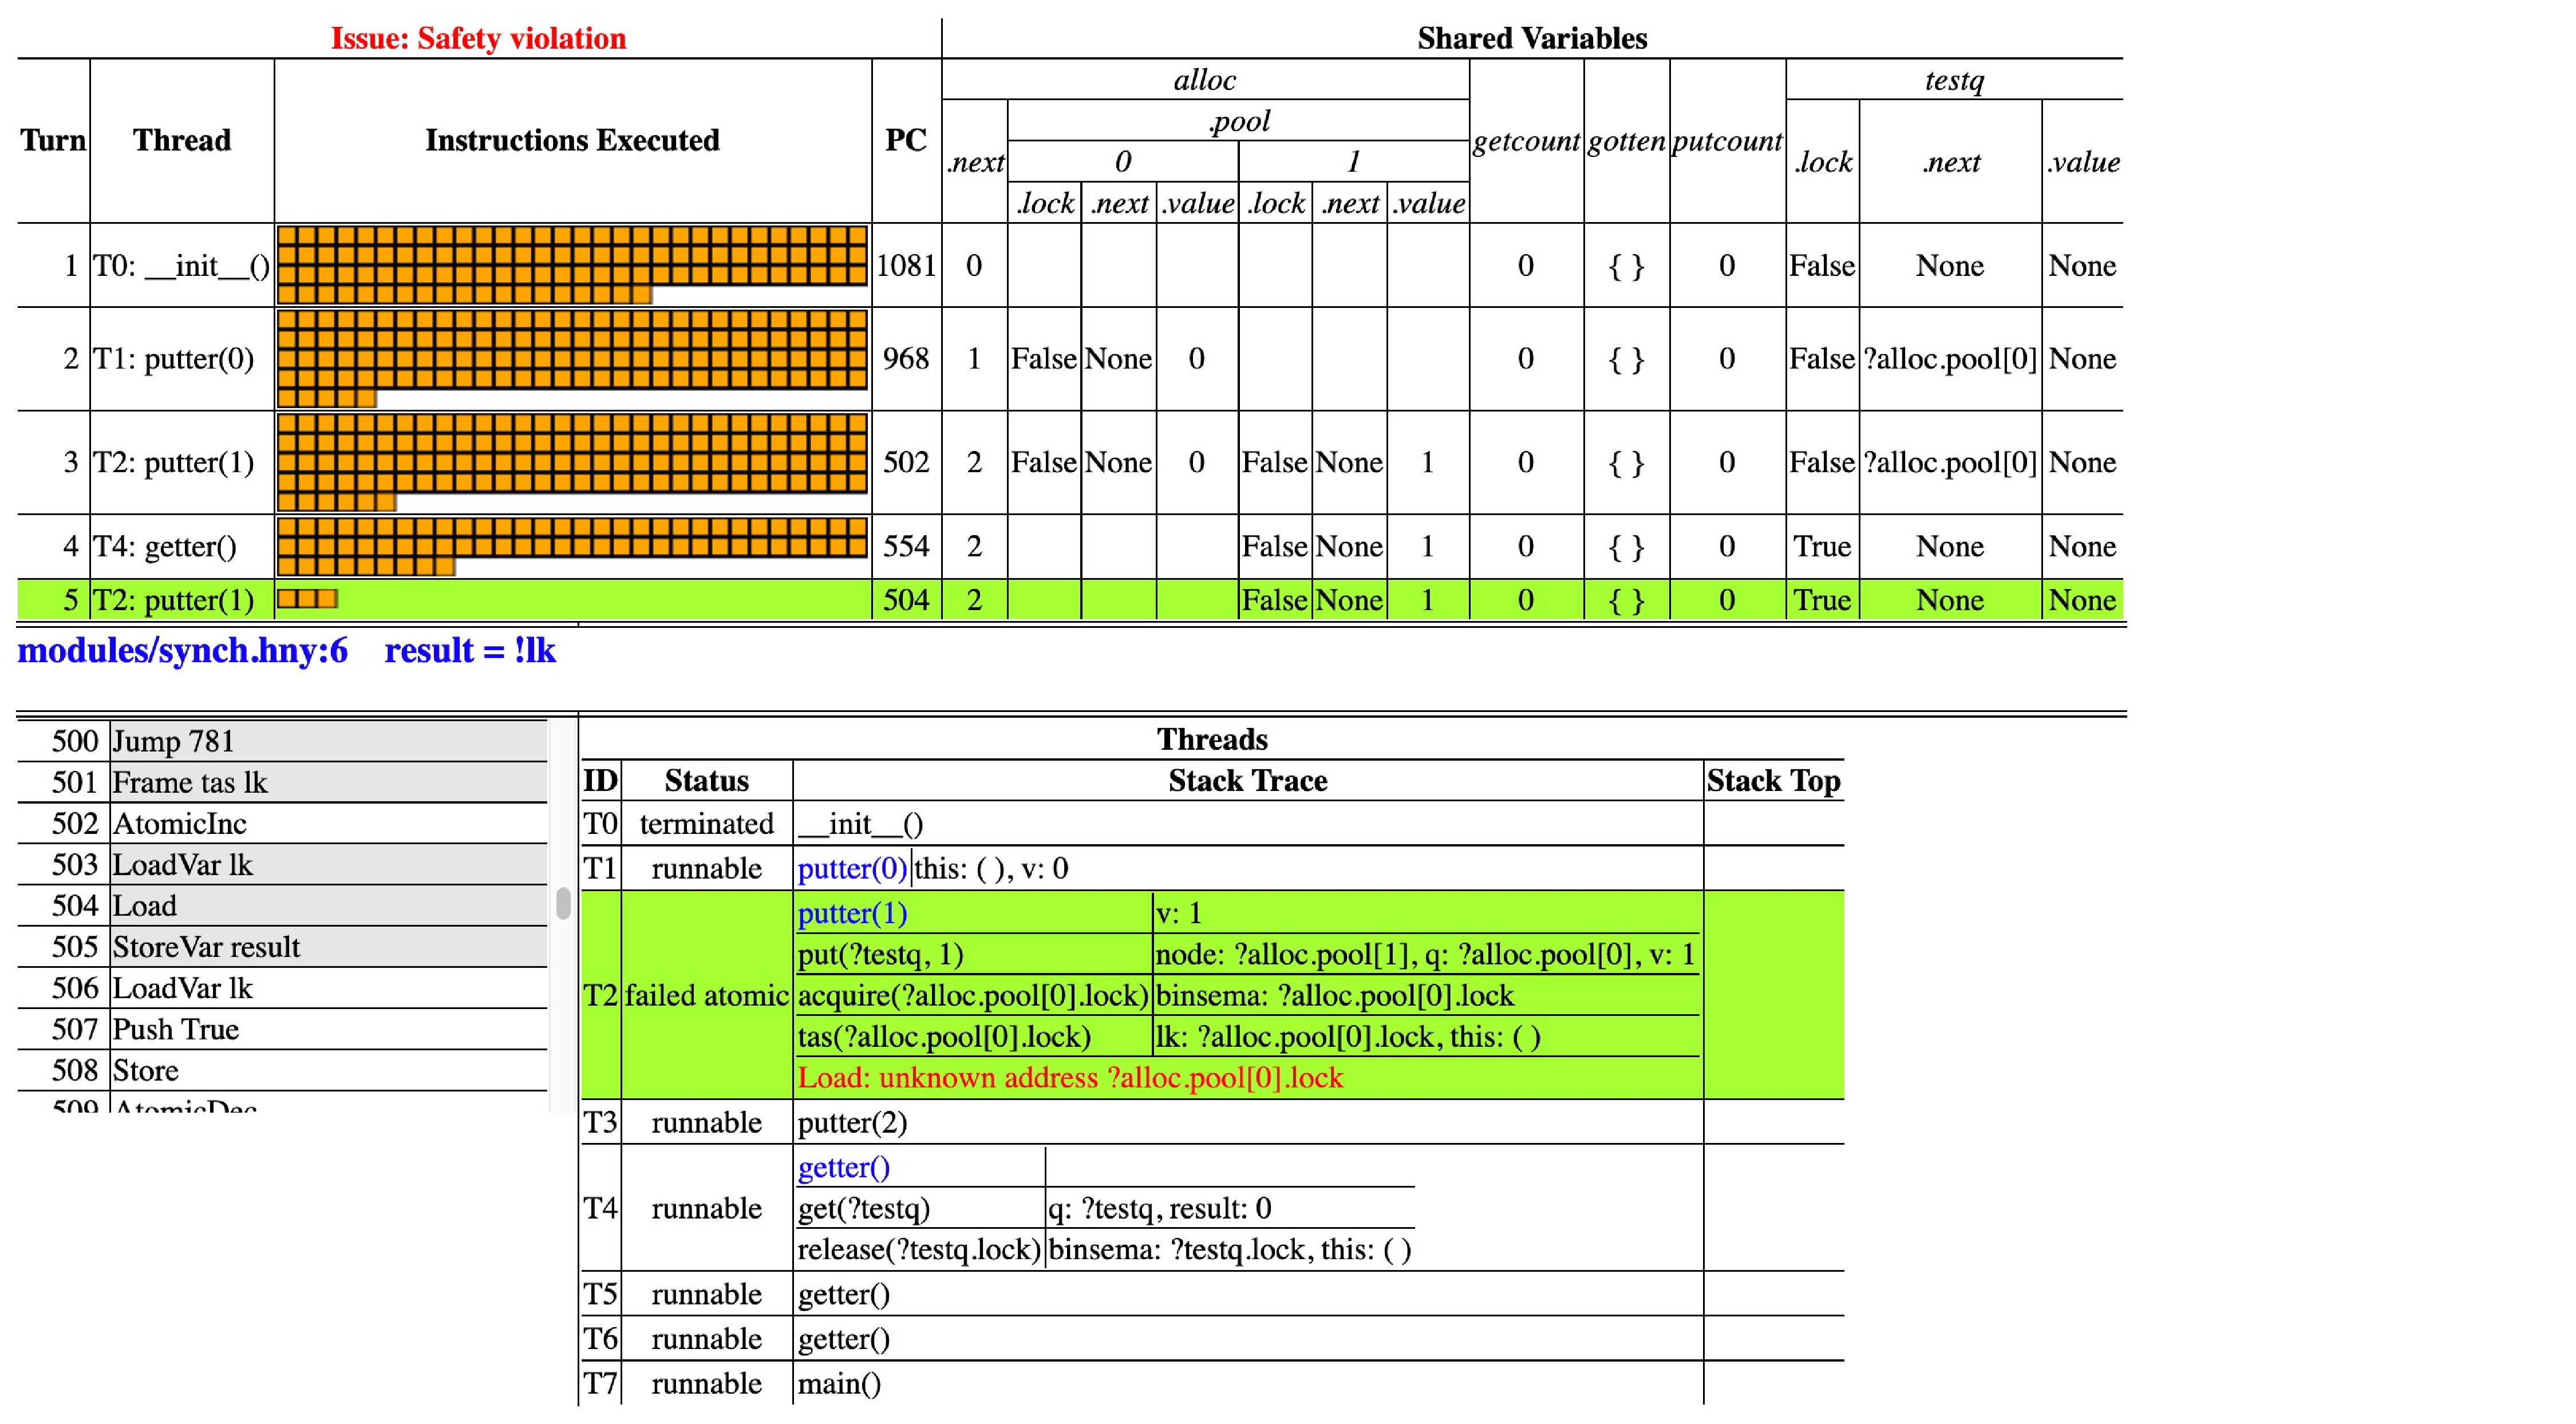
\includegraphics[width=\textwidth]{figures/queuebug1.pdf}
\end{center}
\caption{\harmonyref{queuebug.html}{Harmony output of running \autoref{fig:qtest3} against
\autoref{fig:queuebug}}.}
\label{fig:queuebug1}
\end{figure}

So you wrote a Harmony program and Harmony reports a bug.
Often you may just be able to figure it out by staring at the code and
going through some easy scenarios, but what if you don't?
The output of Harmony can be helpful in that case.

\autoref{fig:queuebug} contains an attempt at a queue implementation
where the queue is implemented by a linked list, with the first node
being a \texttt{dummy} node to prevent data races.  Each node in the
list contains a lock.  The \texttt{put}() method walks the list until
it gets to the last node, each time acquiring the lock to access the
node's fields.  When \texttt{put}() gets to the last node in the list,
it appends a new one.  The \texttt{get}() method locks the first (dummy)
node, removes the second from the list and frees it.  The method returns
the value from the removed node.

Let us run the code through some of the test programs in the last
chapter.  Harmony does not detect any issues with the sequential test
in \autoref{fig:qtestseq}.
(Run this using the \texttt{-m} flag like this:
\texttt{harmony -m queue=queuebug code/qtestseq.hny})
The concurrent \texttt{put} test of
\autoref{fig:qtest1} as well as the concurrent \texttt{get} test of
\autoref{fig:qtest2} also find no problems.  However, when we run
the new queue code through the test in \autoref{fig:qtest3}, Harmony
finds a problem.

\autoref{fig:queuebug1} shows the Harmony output of running
the test in \autoref{fig:qtest3} against the queue code
in \autoref{fig:queuebug}.
There is quite a bit of information in the Harmony output, and it's
important to learn to navigate through it.
Let's start with looking at the red text.  Harmony found a safety
violation (something bad happened during one of the possible executions),
and in particular \texttt{putter}(1) (thread T2) was trying to dereference
\texttt{alloc}.\textit{pool}[0].\texttt{lock} in turn 5.

The \texttt{alloc} module maintains a shared array \textit{pool} that
it uses for dynamic allocation.  Apparently \texttt{putter}(1) tried to access
\textit{pool}[0], but it does not exist, meaning that either it was not
yet allocated, or it had been freed since it was allocated.
When we look at the top half of the figure, we see that in fact
\texttt{putter}(0) (T1) allocated \textit{pool}[0] in turn 2, while
\texttt{getter}() (T4) released it in turn 4.

So how did we get there?  We can start by single stepping through the
actions of \texttt{putter}(0) by clicking on its first block.
By hitting return repeatedly, we can go through the lines of code that
it is executing.  Doing so, we can see that it allocates
\textit{pool}[0] and uses that as the node to contain value 0 and add
this node to the queue \textit{qtest}.  At the end of its turn,
\texttt{putter}(0) has just finished \texttt{put}(0).  Looking at the
state in the top right, everything looks good.  The first node
(\textit{testq}) points to the allocated node with the value 0 in it,
and its \texttt{next} pointer is \textbf{None}.  The locks on both nodes
are released.  So far so good.

Next \texttt{putter}(1) (thread T2) takes a turn.  It gets to line 10 in
\autoref{fig:queuebug} where it's trying to acquire
$q$$\rightarrow$\texttt{lock}.  If we look at the bottom right,
we see that $q$ points to \textit{pool}[0], the node that has value 0
in it.  Again, so far so good.

But before \texttt{putter}(1) obtains
the lock on \textit{pool}[0], \texttt{getter}() (thread T4) starts
running.  \texttt{getter}() acquires the lock on \textit{qtest}, which
still points to \textit{pool}[0].  \texttt{getter} then extracts the
value from \textit{pool}[0] and then releases it.
At this point \textit{pool}[0] no longer exists, but then
\texttt{putter}(1) starts running again from where it left off.
It was about to acquire the lock on \textit{pool}[0], but now that
node no longer exists.

To fix the code without changing the data structure, we can use
hand-over-hand locking (\autoref{ch:cds}).
\autoref{fig:queuefix} shows an implementation
that uses hand-over-hand locking
both for \texttt{put}() and for \texttt{get}().  It passes all tests.

\begin{figure}
\begin{code}
\harmonysource{queuefix}
\end{code}
\caption{\harmonylink{code/queuefix.hny} Queue implementation with hand-over-hand locking.}
\label{fig:queuefix}
\end{figure}

\chapter{Conditional Waiting}
\label{ch:condwait}

Critical sections enable multiple threads
to easily share data structures whose modification
requires multiple steps.
A critical section only allows one thread to execute the code
of the critical section at a time.
Therefore, when a thread arrives at a critical section,
the thread blocks until there is no other thread in the critical section.

\glsadd{busy waiting}%
\index{busy waiting}%
Sometimes it is useful for a thread to block waiting for additional
conditions.
For example, when dequeuing from an empty shared queue,
it may be useful for the thread to block until the queue is non-empty
instead of returning an error.
The alternative would be \emph{busy waiting} (aka \emph{spin-waiting}),
where the thread repeatedly tries to dequeue an item until it is successful.
Doing so wastes CPU cycles and adds contention to queue access.
%
A thread that is busy waiting until the queue is non-empty cannot
make progress until another thread enqueues an item.
However, the thread is not considered \emph{blocked} because it is
changing the shared state by repeatedly acquiring and releasing the
lock.
We distinguish \emph{passive busy waiting} and \emph{active busy waiting}.
A process that is waiting for a condition without changing the state
(like in a spinlock) is passively busy waiting.
A process that is waiting for a condition while changing the state
(such as repeatedly trying to dequeue an item, which requires
acquiring a lock) is actively busy waiting.

We would like to find a solution to \emph{conditional waiting}
so that a thread blocks until the condition holds---or at least most
of the time.
Before we do so, we will give two classic examples of synchronization
problems that involve conditional waiting: \emph{reader/writer locks}
and \emph{bounded buffers}.

\begin{figure}
\begin{code}
\harmonysource{RWtest}
\end{code}
\caption{\harmonylink{code/RWtest.hny} Test code for reader/writer locks.}
\label{fig:rwtest}
\end{figure}

\section{Reader/Writer Locks}
\index{reader/writer lock}%
\glsadd{reader/writer lock}%

\begin{comment}
\begin{figure}
\begin{code}
\harmonysource{RW}
\end{code}
\caption{\harmonylink{code/RW.hny} Busy-Waiting Reader/Writer Lock implementation.}
\label{fig:rwbusy}
\end{figure}

\begin{figure}
\begin{center}
\includegraphics[width=2.3in]{figures/rdwr.png}
\end{center}
\caption{High-level state diagram specification of reader/writer locks with
up to two threads.
The first number in a state gives the number of threads; the second number is the
number of threads reading in the critical section; the third is the number of
threads writing in the critical section.}
\label{fig:rdwr}
\end{figure}
\end{comment}

Locks are useful when accessing a shared data structure.  By preventing
more than one thread from accessing the data structure at the same
time, conflicting accesses are avoided.  However, not all concurrent
accesses conflict, and opportunities for concurrency may be lost,
hurting performance.  One important case is when multiple threads
are simply reading the data structure.
In many applications, reads are the majority of all accesses,
and read operations do not conflict with one another.
Allowing reads to proceed concurrently can significantly improve performance.

What we want is a special kind of lock that allows either (i) one writer
or (ii) one or more readers to acquire the lock.  This is called
a \emph{reader/writer lock}~\cite{CHP71}.
%
A reader/writer lock is an object whose abstract (and opaque)
state contains two integer counters:
\begin{enumerate}
\item \textit{nreaders}: the number of readers
\item \textit{nwriters}: the number of writers
\end{enumerate}
satisfying the following invariant:
\begin{itemize}
\item [] $(\mathit{nreaders} \ge 0 \land \mathit{nwriters} = 0) \lor
    (\mathit{nreaders} = 0 \land 0 \le \mathit{nwriters} \le 1)$
\end{itemize}

There are four operations on a reader/writer lock \textit{rw}:
\begin{itemize}
\item \texttt{read\_acquire}(\textit{rw}): waits until $\mathit{nwriters} = 0$
and then increments \textit{nreaders};
\item \texttt{read\_release}(\textit{rw}): decrements $\mathit{nreaders}$;
\item \texttt{write\_acquire}(\textit{rw}): waits until
$\mathit{nreaders} = \mathit{nwriters} = 0$
and then sets \textit{nwriters} to 1;
\item \texttt{write\_release}(\textit{rw}): sets $\mathit{nwriters}$ to 0.
\end{itemize}

\autoref{fig:rwtest} shows how reader/writer locks operations
may be tested.
Similar to ordinary locks, a thread is restricted in how it is allowed to
invoke these operations.
In particular, a thread can only release a reader/writer lock for reading
if it acquired it for reading and the same for writing.
Moreover, a thread is only allowed the acquire a reader/writer lock once.

\begin{comment}
We will explore various ways of implementing reader/writer locks in
this chapter and future ones.

\autoref{fig:rwbusy} presents a solution that uses a
single (ordinary) lock and two counters: one that maintains the number
of readers and one that maintains the number of writers.
\autoref{fig:rwtest} shows how the code may be used.
We will call the lock the \emph{mutex} to distinguish it clearly from
the reader/writer lock that we are implementing.
The mutex is used to protect shared access to the counters.
The program shows a thread that executes in a loop.
Each time, it decides whether to read or write.
The critical section is spread between two labels:
readers access \texttt{@rcs} and writers access \texttt{@wcs}.
The specification is that if a reader is at label \texttt{@rcs},
no writer is allowed to be at label \texttt{@wcs}.  Vice versa, if
a writer is at label \texttt{@wcs}, no reader is allowed to be at
label \texttt{@rcs} \emph{and} there cannot be another writer at
label \texttt{@wcs}.

\autoref{fig:rdwr} shows a high-level
specification for two threads.

A thread that wants to read first waits until there are no writers:
\textit{nwriters} == 0.  Then it increments the number of readers.
Similarly, a
thread that wants to write waits until there are no readers \emph{or} writers.
Then it increments the number of writers.
The important invariants in this code are:
\begin{itemize}
\item $n$ readers at \texttt{@rcs} $\Rightarrow \mathit{nreaders} \ge n$,
\item $n$ writers at \texttt{@wcs} $\Rightarrow \mathit{nwriters} \ge n$,
\item $(\mathit{nreaders} \ge 0 \land \mathit{nwriters} = 0) \lor
    (\mathit{nreaders} = 0 \land 0 \le \mathit{nwriters} \le 1)$.
\end{itemize}
It is easy to see that the invariants hold and imply the reader/writer
specification.
The solution also supports progress: if no thread is in the critical
section then any thread can enter.  Better still: if any reader is in the
critical section, any other reader is also able to enter.

\begin{figure}
\begin{code}
\harmonysource{RWbusychk}
\end{code}
\caption{\harmonylink{code/RWbusychk.hny} Checking for Busy Waiting.}
\label{fig:rwblock}
\end{figure}

\glsadd{busy waiting}%

While correct, it is not considered a good solution.
The solution is an example of what is called \emph{busy-waiting}
\index{busy waiting}%
(aka \emph{spin-waiting}):
\index{spin waiting}%
threads spin in a loop until some desirable application-level condition is met,
wasting CPU cycles.
\autoref{fig:inc} also has an example of busy-waiting: the \texttt{main}
thread waits for the other two threads to finish by checking their \texttt{done}
flags.

The astute reader might wonder if obtaining the mutex itself is an
example of busy-waiting.  After all, the Harmony \texttt{synch} implementation
of \texttt{lock()} spins in a loop until the mutex is available
(see \autoref{fig:spinlocks}).
However, there is a big difference.  As we pointed out, the threads that
are waiting for a spinlock are \emph{blocked}.
In most operating systems and programming language runtimes,
when a thread acquires a mutex, the thread is placed on a scheduling
queue and stops using CPU cycles until the mutex becomes available.
Harmony supports this with the \texttt{synchS} module.
Busy waiting disables all this: even when using the \texttt{synchS}
module, readers and writers only get suspended temporarily in case
there is contention for the mutex.
A thread trying to obtain a read or write lock in
\autoref{fig:rwbusy} tries to obtain the mutex repeatedly.

Thus, it is considered ok to have threads be blocked while waiting
for application-specific conditions, but not for them to
busy-wait for application-specific conditions.

Harmony does not complain about \autoref{fig:rwbusy}, but, using
the right test, Harmony can be used to check for busy-waiting.
\autoref{fig:rwblock} presents such a test.
Note that the initialization code obtains a write lock, preventing
all readers and writers from entering the critical section.
In that case, those threads should ideally be blocked and Harmony
can test for that by running it with the \texttt{-b} flag.
This flag tells Harmony to check
that all states are non-terminating and lead to a state in which
all threads are blocked.

\section*{Exercises}
\begin{problems}
\item Draw additional states and steps in \autoref{fig:rdwr}
for three threads.
\end{problems}

\chapter{Reader/Writer Locks with Blocking}
\label{ch:rdwr}

\begin{figure}
\begin{code}
\harmonysource{RWlock}
\end{code}
\caption{\harmonylink{code/RWlock.hny} Reader/Writer with Two Locks.}
\label{fig:rw2lock}
\end{figure}

\begin{figure}
\begin{code}
\harmonysource{RWmulti}
\end{code}
\caption{\harmonylink{code/RWmulti.hny} Checking that multiple readers can acquire the read lock.}
\label{fig:rwmulti}
\end{figure}

\autoref{fig:rw2lock} presents a reader/writer lock implementation
that does not busy-wait.
You can test the code by running \texttt{harmony -m RW=RWlock RWtest.hny}.
It uses two ordinary locks: \textit{rwlock} is used by both readers and writers,
while \textit{rlock} is only used by readers.
\textit{rwlock} is held either when readers are at label \texttt{@rcs}
or when a writer is at label \texttt{@wcs}.
\textit{rlock} is used to protect the \textit{nreaders} variable that
counts the number of readers in the critical section. 

The invariants that imply the reader/writer specification
(which are again easy to verify) are as follows:

\begin{itemize}
\item $n$ readers at \texttt{@rcs} $\Rightarrow \mathit{nreaders} \ge n$
\item $\exists$ writer at \texttt{@wcs} $\Rightarrow \mathit{nreaders} = 0$ and writer holds \textit{rwlock}
\item at most one writer can hold \textit{rwlock}
\end{itemize}

A writer just acquires \textit{rwlock} to enter the critical section
and releases it to exit.  The \emph{first} reader to enter the critical
section acquires \textit{rwlock} and the \emph{last} reader to exit
the critical section releases \textit{rwlock}.
The implementation satisfies progress: if no thread is in the critical
section then any thread can enter.

It is instructive to see what happens when a writer is in the critical
section and two readers try to enter.  The first reader successfully
acquires \textit{rlock} but blocks when trying to acquire
\textit{rwlock}, which is held by the writer.  The second reader blocks
trying acquire \textit{rlock} because it is held by the first reader.
When the writer leaves the critical section, the first reader acquires
\textit{rwlock}, sets \textit{nreaders} to 1, and releases \textit{rlock}.
\textit{rwlock} is still held.
Then the second reader acquires \textit{rlock} and, assuming the first
reader is still in the critical section, increments \textit{nreaders} to 2
and enters the critical section \emph{without} acquiring \textit{rwlock}.
\textit{rwlock} is essentially jointly held by both readers.
It does not matter in which order they leave: the second will release
\textit{rwlock}.

While Harmony does not detect any issues, we must remember what it is checking
for: it checks to make sure that there are never a reader and a writer
in the critical section, and there are never two writers in the critical
section.  Moreover, it checks progress: all executions eventually terminate.
What it does \emph{not} check is if the code allows more than one reader
in the critical section.  Indeed, we could have implemented the reader/writer
lock using an ordinary lock, never allowing
more than one thread in the critical section, and Harmony would not have
complained.

\autoref{fig:rwmulti} contains a new test that ensures that indeed more
than one reader can enter the critical section at a time.  It does so by
having threads sometimes wait in the critical section until all other readers
are there.  If other readers cannot enter, then that thread enters in an
infinite loop that Harmony will readily detect.  Try it out!

An important lesson here is that one should not celebrate too early if Harmony
does not find any issues.  While a test may be successful, a test may not
explore all desirable executions.  While Harmony can help explore all cornercases
in a test, it cannot find problems that the test is not looking for.

\section*{Exercises}
\begin{problems}
\item Why do you suppose the code in \autoref{fig:rwmulti} uses a flag
per thread rather than a simple counter?
Can you write a version of this test that uses a counter instead
of a flag per thread?
% \item Write a ``library implementation'' of reader/writer locks so multiple
% reader/writer locks can be instantiated.
\end{problems}

\chapter{Semaphores}
\label{ch:semaphore}
\index{semaphore}%

\glsadd{semaphore}%

\begin{figure}
\begin{code}
\harmonysource{semaphore}
\end{code}
\caption{\harmonylink{modules/synch.hny} The \texttt{Semaphore} interface in the \texttt{synch} module.}
\label{fig:semaphore}
\end{figure}

\begin{figure}
\begin{code}
\harmonysource{DinersSema}
\end{code}
\caption{\harmonylink{code/DinersSema.hny} Italian Philosophers.}
\label{fig:dinerssema}
\end{figure}

So far, we have looked at how to protect a single resource.
Some types of resources may have multiple units.
If there are only $n$ units, no more than $n$ units can be used at a time;
if all are in use and a thread comes along that needs one of the units,
it has to wait until another thread releases one of the units.
Note that we cannot solve this problem simply using a lock per unit---allocating
a unit requires access to the entire collection.

Consider the following synchronization problem that we call
\emph{Italian Philosophers} (a simplification of
the famous Dining Philosophers problem described in \autoref{ch:deadlock}).
There are five philosophers sitting around a table, each with a plate of
spaghetti in front of them.
There is a glass sitting in the middle of the table with only
three forks in it.  A philosopher needs one of those forks to eat, but clearly,
no more than three philosophers can eat at a time.
Unfortunately, a lock can only count to one.

Introduced by Dijkstra,
a \emph{semaphore} is a synchronization primitive that
can solve this kind of problem~\cite{EWD35}.
A semaphore is essentially
a counter that can be incremented and decremented but is not allowed to go
below zero.  The semaphore counter is typically initialized to the number of
units of a resource initially available.
When allocating a resource, a thread decrements the
counter using the \texttt{P}
\index{P}%
\index{procure}%
operation.  You can think of \texttt{P} standing
for \emph{Procure}, as in procuring the resource associated with the semaphore.
The \texttt{P} operation blocks the invoking thread if the counter is zero.
To release the resource, a thread increments the resource using the
\texttt{V}
\index{V}%
\index{vacate}%
operation.  You can think of \texttt{V} standing for \emph{vacate},
as in vacating the resource.
One can think of a semaphore as a generalization of a lock.  In fact, a
lock can be implemented by a semaphore initialized to 1.  Then \texttt{P}
procures the lock, and \texttt{V} vacates the lock.

\autoref{fig:semaphore} shows the \texttt{synch} module implementation of
semaphores.
It represents a semaphore as an integer.
\autoref{fig:dinerssema} shows a solution to the Italian Philosphers problem
using a semaphore.

You may find the free ``The Little Book of Semaphores'' by
Allen Downey a great resource for working with semaphores~\cite{Downey09}.

\section*{Exercises}
\begin{problems}
\item How might you check with Harmony that at most three
Italian philosophers can eat at the same time?
\item Implement a test program that checks to see that
the solution allows more than one Italian philosopher to eat at the same time?
\end{problems}
\end{comment}

\section{Bounded Buffer}
\index{bounded buffer}%
\index{producer/consumer problem}%
\glsadd{producer/consumer problem}%

\begin{comment}
\begin{figure}
\begin{center}
\includegraphics[width=2.5in]{figures/pc-crop.pdf}
\end{center}
\caption{High-level state diagram specification of producers/consumers.}
\label{fig:pc}
\end{figure}

\begin{figure}
\begin{code}
\harmonysource{BBsema}
\end{code}
\caption{\harmonylink{code/BBsema.hny} Bounded Buffer implementation using semaphores.}
\label{fig:boundedbuffer}
\end{figure}

\begin{figure}
\begin{code}
\harmonysource{BBsematest}
\end{code}
\caption{\harmonylink{code/BBsematest.hny} Test program for \autoref{fig:boundedbuffer}.}
\label{fig:bbtest}
\end{figure}

\begin{figure}
\begin{code}
\begin{verbatim}
harmony -b -c NSLOTS=0 -c NPRODS=1 -c NCONSS=1 BBsematest.hny
harmony -b -c NSLOTS=1 -c NPRODS=0 -c NCONSS=1 BBsematest.hny
harmony    -c NSLOTS=1 -c NPRODS=1 -c NCONSS=0 BBsematest.hny
harmony    -c NSLOTS=1 -c NPRODS=1 -c NCONSS=1 BBsematest.hny
harmony -b -c NSLOTS=1 -c NPRODS=1 -c NCONSS=2 BBsematest.hny
harmony -b -c NSLOTS=1 -c NPRODS=2 -c NCONSS=0 BBsematest.hny
harmony    -c NSLOTS=1 -c NPRODS=2 -c NCONSS=1 BBsematest.hny
harmony    -c NSLOTS=1 -c NPRODS=2 -c NCONSS=2 BBsematest.hny
harmony -b -c NSLOTS=1 -c NPRODS=2 -c NCONSS=3 BBsematest.hny
harmony    -c NSLOTS=2 -c NPRODS=1 -c NCONSS=0 BBsematest.hny
harmony    -c NSLOTS=2 -c NPRODS=1 -c NCONSS=1 BBsematest.hny
harmony -b -c NSLOTS=2 -c NPRODS=1 -c NCONSS=2 BBsematest.hny
harmony    -c NSLOTS=2 -c NPRODS=2 -c NCONSS=0 BBsematest.hny
harmony    -c NSLOTS=2 -c NPRODS=2 -c NCONSS=1 BBsematest.hny
harmony    -c NSLOTS=2 -c NPRODS=2 -c NCONSS=2 BBsematest.hny
harmony -b -c NSLOTS=2 -c NPRODS=2 -c NCONSS=3 BBsematest.hny
harmony -b -c NSLOTS=2 -c NPRODS=3 -c NCONSS=0 BBsematest.hny
harmony    -c NSLOTS=2 -c NPRODS=3 -c NCONSS=1 BBsematest.hny
harmony    -c NSLOTS=2 -c NPRODS=3 -c NCONSS=2 BBsematest.hny
harmony    -c NSLOTS=2 -c NPRODS=3 -c NCONSS=3 BBsematest.hny
\end{verbatim}
\end{code}
\caption{Script for testing producer/consumer synchronization.}
\label{fig:pcscript}
\end{figure}
\end{comment}

\index{ring buffer}%
A \emph{bounded buffer} (aka \emph{ring buffer}) is
a queue with the usual \texttt{put/get} interface,
but implemented using a circular buffer
\index{circular buffer}%
of a certain length and two pointers:
the \emph{tail} points where new items are enqueued and the \emph{head}
points where items are dequeued.
If the buffer is full, the enqueuer must wait; if the buffer is empty, the
dequeuer must wait.
This problem is known as the ``Producer/Consumer Problem'' and was
proposed by Dijkstra~\cite{EWD329}.
Multiple producers and multiple consumers may all share
the same bounded buffer.

The producer/consumer pattern is common.  Threads may be arranged
in \emph{pipelines},
\index{pipeline}%
where each upstream thread is a producer and each downstream
thread is a consumer.
Or threads may be arranged in a manager/worker pattern, with a manager
producing jobs and workers consuming and executing them in parallel.
Or, in the client/server model,
\index{client/server model}%
some thread may act as a \emph{server} that clients can send requests to
and receive responses from.  In that case, there is a bounded buffer
for each client/server pair. Clients produce requests and
consume responses, while the server consumes requests and produces responses.

\begin{comment}
\autoref{fig:pc} gives a high-level description.  The
two numbers in a state specify
the number of items that the producers still can produce and
the number of items that the consumers have consumed.  In this
description there are three items to produce initially.

\begin{figure}
\begin{code}
\harmonysource{BBsemadata}
\end{code}
\caption{\harmonylink{code/BBsemadata.hny} Test whether the bounded buffer delivers the right data in the
right order.}
\label{fig:BBsemadata}
\end{figure}

\autoref{fig:boundedbuffer} presents the implementation of a bounded
buffer using semaphores.  It features a circular bounded buffer \textit{buf} with
slots numbered 1 through \texttt{NSLOTS}.  There are two indexes into
the buffer: \textit{b\_in} specifies where the next produced item is inserted,
while \textit{b\_out} specifies from where the next can be consumed.
As there may be multiple producers and multiple
consumers, updates to the indexes, which are shared variables, must be protected.
To this end, we use two semaphores as locks: \textit{l\_in} for \textit{b\_in}
and \textit{l\_out} for \textit{b\_out}.

Without additional synchronization, the indexes may overflow and point to invalid
entries in the circular buffer.
For this, there is a semaphore \textit{n\_full} that
keeps track of the number of filled entries in the buffer and a semaphore
\textit{n\_empty} that keeps track of the number of empty entries in the buffer.

To add an item to the bounded buffer (\texttt{produce}(\textit{item})), the producing
thread first has to wait until there is room in the bounded buffer.
To this end, it invokes \texttt{P}(\textit{n\_empty}), which waits until
$\mathit{n\_empty} > 0$ and atomically decrements \textit{n\_empty} once this
is the case.  In other words, the producer procures an empty slot.
Next, it adds the item to the next position in the buffer.
Since there may be more than one empty slot, multiple producers may attempt
to do the same thing concurrently.  Hence the use of the \textit{l\_in}
semaphore used as a lock.  Finally, once the item is added, the thread
increments the \textit{n\_full} semaphore to signal to consumers that
an item is available.
The consumer code is symmetric.

Note the quite different usage of the \textit{l\_} semaphores and \textit{n\_}
semaphores.
People often call semaphores that are used as locks \emph{binary semaphores},
\index{binary semaphore}%
as they only take on the values 0 and 1.
They protect critical sections.
The second type of semaphores are called \emph{counting semaphores}.
\index{counting semaphore}%
They can be used to send signals between threads.
However, binary and counting semaphores are implemented the same way.

\autoref{fig:bbtest} invokes the code of \autoref{fig:boundedbuffer}.
We can run this through Harmony, but what would it test?  There are
no assert statements in the code.  We can split the functionality
of this code into two and test each separately.  One is the
synchronization part: producers should never run more than
\texttt{NSLOTS} ahead of the consumers, but they should be able to
produce up to \texttt{NSLOTS} items even if there are no consumers.
The other part is the data: we want to make sure that the items are
sent through the buffer in order and without loss.  We will first
focus on the synchronization.

The first part can be tested with the code given in \autoref{fig:pc}, by
experimenting with different non-negative values for the three constants.
In particular, any run with a positive \texttt{NSLOTS} and
$\mathtt{NCONSS} \le \mathtt{NPRODS} \le \mathtt{NCONSS} + \mathtt{NSLOTS}$
should terminate, while other values should lead to threads blocking.
To this this, one can write a script like the one in \autoref{fig:pcscript}.

\autoref{fig:BBsemadata} tests whether the correct data is sent in
the correct order.  There are the same number of producers and consumers.
Each producer $i$ produces two tuples: $(i, 0)$ and $(i, 1)$ in that order.
Each consumer consumes two tuples and checks that the tuples are different
and that, if the two tuples come from the same producer, then they have to
be in the order sent.
Moreover, consumers add the tuples they received to the set
\textit{received} (atomically---a lock could have been used here as well).
The \texttt{main()} thread waits for all consumers to have received
exactly the set of tuples that the producers produce.

\section*{Exercises}
\begin{problems}
\end{problems}
\end{comment}

\chapter{Split Binary Semaphores}
\label{ch:sbs}
\index{split binary semaphore}%

\begin{figure}
\begin{code}
\harmonysource{RWsbs}
\end{code}
\caption{\harmonylink{code/RWsbs.hny} Reader/Writer Lock using Split Binary Semaphores.}
\label{fig:RWsplitsema}
\end{figure}

\glsadd{conditional critical section}%

The Split Binary Semaphore (SBS) approach is a general technique for
implementing conditional waiting.  It was originally proposed by
Tony Hoare and popularized by Edsger Dijkstra~\cite{EWD703}.
SBS is an extension of a critical section that is protected by a single
binary semaphore.
If there are $n$ \emph{waiting conditions},
then SBS uses $n+1$ binary semaphores to protect the critical section.
An ordinary critical section has no waiting conditions.
For example, a bounded buffer has two waiting conditions:
\begin{enumerate}
\item consumers waiting for the buffer to be non-empty;
\item producers waiting for an empty slot in the buffer.
\end{enumerate}
So, it will require 3 binary semaphores if the SBS technique is applied.

Think of each of these semaphores as a gate that a thread must go
through in order to enter the critical section.  A gate is either open
or closed.  Initially, exactly one gate, the main gate, is open.
Each of the other gates, the \emph{waiting gates}, is associated with a
waiting condition.
When a gate is open, one thread can enter the critical section,
closing the gate behind it.

When leaving the critical section, the thread must open exactly one
of the gates, but it does not have to be the gate that it used to enter
the critical section.
In particular, when a thread leaves the critical section it should
check for each waiting gate if its waiting condition holds and if there are
threads trying to get through the gate.  If there is such a gate,
it must select one and open that gate.  If there is no such gate,
it must open the main gate.

Finally, if a thread is executing in the critical section and needs to
wait for a particular condition, it leaves the critical section and waits
for the gate associated with that condition to open.

Note that the following invariants hold:
\begin{itemize}
\item At any time, at most one gate is open;
\item If some gate is open, then no thread is in the critical section.  Equivalently, if some thread is in the critical section, all gates are closed;
\item At any time, at most one thread is in the critical section.
\end{itemize}

The main gate is implemented by a binary semaphore, initialized in the
released state (signifying that the gate is open).
The waiting gates each consist of a pair: a counter that counts how many
threads are waiting behind the gate and a binary semaphore initialized
in the acquired state (signifying that the gate is closed).

We will illustrate the technique using the reader/writer problem.
\autoref{fig:RWsplitsema} shows code.
The first step is to enumerate all waiting conditions.
In the case of the reader/writer
problem, there are two: a thread that wants to read may have to wait for a
writer to leave the critical section, while a thread that wants to write may
have to wait until all readers have left the critical section or until a writer has left.
%
The state of a reader/writer lock thus consists of the following:
\begin{itemize}
\item \textit{nreaders}: the number of readers in the critical section;
\item \textit{nwriters}: the number of writers in the critical section;
\item \textit{mutex}: the main gate binary semaphore;
\item \textit{r\_gate}: the waiting gate used by readers, consisting of a binary semaphore and the number of readers waiting to enter;
\item \textit{w\_gate}: the waiting gate used by writers, similar to the readers' gate.
\end{itemize}

Each of the
\texttt{read\_acquire}, \texttt{read\_release},
\texttt{write\_acquire}, and \texttt{write\_release} methods must maintain
this state.
First they have to acquire the \textit{mutex}
(i.e., enter the main gate).
After acquiring the \textit{mutex},
\texttt{read\_acquire} and \texttt{write\_acquire} each must check to see
if it has to wait.
If so, it increments the count associated with its respective gate,
opens a gate (using method \texttt{release\_one}), and then blocks until
its waiting gate opens up.

\texttt{release\_one()} is the function that a thread uses when leaving
the critical section.  It must check to see if there is a waiting gate
that has threads waiting behind it and whose condition is met.
If so, it selects one and opens that gate.  In the given code,
\texttt{release\_one()} first checks the readers' gate and then the
writers' gate, but the other way around would have worked as well.
If neither waiting gate qualifies, then \texttt{release\_one()} 
has to open the main gate (i.e., release \textit{mutex}).

Let us examine \texttt{read\_acquire} more carefully.
First the method acquires the \textit{mutex}.
Then, in the case that the thread
finds that there is a writer in the critical section
($\mathit{nwriters > 0}$), it increments the counter associated with
the readers' gate, leaves the critical section (\texttt{release\_one}),
and then tries to acquire the semaphore associated with the waiting gate.
This will cause it to block until some thread opens that gate.

Now consider the case where there is a writer in the critical
section and there are two readers waiting.  Let us see what happens when
the writer calls \texttt{write\_release}:
\begin{enumerate}
\item After acquiring \textit{mutex}, the writer decrements
\textit{nwriters}, which must be 1 at this time, and thus becomes 0.
\item It then calls \texttt{release\_one()}.
\texttt{release\_one()} finds that there are no writers in the critical section
and there are two readers waiting.  It therefore releases not
\textit{mutex} but the readers' gate's binary semaphore.
\item One of the waiting readers can now re-enter the critical section.
When it does, the reader decrements the gate's counter (from 2 to 1)
and increments \textit{nreaders} (from~0 to~1).
The reader finally calls \texttt{release\_one()}.
\item Again, \texttt{release\_one()} finds that there are no writers and
that there are readers waiting, so again it releases the readers' semaphore.
\item The second reader can now enter the critical section.
It decrements the gate's count from 1 to 0 and increments \textit{nreaders}
from~1 to~2.
\item Finally, the second reader  calls \texttt{release\_one()}.
This time \texttt{release\_one()} does not find any threads waiting,
and so it releases \textit{mutex}.
There are now two threads that are holding the reader/writer lock.
\end{enumerate}

\section*{Exercises}
\begin{problems}
% \item Assume that you have only binary semaphores.
% Implement counting semaphores using the split binary semaphores technique.
\item Several of the instantiations of \texttt{release\_one()} in
\autoref{fig:RWsplitsema} can be replaced by simply releasing \textit{mutex}.
Which ones?
\item Optimize your solutions to \autoref{ex:qcontains} to use reader/writer locks.
\item \label{ex:bbsbs} Implement a solution to the producer/consumer problem
using split binary semaphores.
\item \label{ex:boundlock} Using busy waiting, implement a ``bound lock'' that allows
up to \texttt{M} threads to acquire it at the same time.\footnote{A bound lock is a restricted version of a \emph{counting} semaphore.}
A bound lock
with \texttt{M == 1} is an ordinary lock.
You should define a constant \texttt{M} and two methods:
\texttt{acquire\_bound\_lock()}
and \texttt{release\_bound\_lock()}.
(Bound locks are useful for situations where too many threads working
at the same time might exhaust some resource such as a cache.)
\item Write a test program for your bound lock
that checks that no more than \texttt{M} threads can acquire the
bound lock.
\item Write a test program for bound locks
that checks that up to \texttt{M} threads
can acquire the bound lock at the same time.
% \item Implement a \emph{bounded stack}.  Method \texttt{push}(\textit{item})
% should block if the stack is full.  Method \texttt{pop()} should block
% until the stack is non-empty and then return an item.
% Also implement test programs for your solution.
\item \label{ex:gpu} Implement a thread-safe \emph{GPU allocator} by modifying
\autoref{fig:gpu}.
There are \texttt{N} GPUs identified by the numbers
1 through \texttt{N}.  Method \texttt{gpuAlloc()} returns the identifier
of an available GPU, blocking if there is currently no available GPU.
Method \texttt{gpuRelease}(\textit{gpu}) releases the given GPU.  It never needs
to block.
\item With reader/writer locks,
concurrency can be improved if a thread \emph{downgrades} its write lock
to a read lock when its done writing but not done reading.  Add
a \texttt{downgrade} method to the code in \autoref{fig:RWsplitsema}.
(Similarly, you may want to try to implement an \emph{upgrade} of a
read lock to a write lock.  Why is this problematic?)
% How easy or hard would it be to do the same for the code in
% \autoref{fig:rw2lock}?
% Note, you cannot simply release the
% write lock and then obtain the read lock, because the thread needs
% to remain in the critical section.
\item \label{ex:onelane} Cornell's campus features some one-lane bridges.
On a one-lane bridge,
cars can only go in one direction at a time. Consider northbound
and southbound cars wanting to cross a one-lane bridge.
The bridge allows arbitrary many cars, as long as they're going in the
same direction.
Implement a lock that observes this requirement using SBS.
Write methods \texttt{OLBlock()} to create a new ``one lane bridge'' lock,
\texttt{nb\_enter()} that a car must invoke before going northbound on
the bridge and \texttt{nb\_leave()} that the car must invoke after leaving
the bridge.  Similarly write \texttt{sb\_enter()} and \texttt{sb\_leave()}
for southbound cars.
\item Extend the solution to \autoref{ex:onelane} by implementing the
requirement that at most $n$ cars are allowed on the bridge.  Add $n$
as an argument to \texttt{OLBlock}.

\end{problems}

\begin{figure}
\begin{code}
\harmonysource{gpu}
\end{code}
\caption{\harmonylink{code/gpu.hny} A thread-unsafe GPU allocator.}
\label{fig:gpu}
\end{figure}

\chapter{Starvation}
\label{ch:starvation}
\index{starvation}%

\glsadd{starvation}%

\begin{figure}
\begin{code}
{\small
\harmonysource{RWfair}
}
\end{code}
\caption{\harmonylink{code/RWfair.hny} Reader/Writer Lock SBS implementation addressing fairness.}
\label{fig:RWfair}
\end{figure}

\glsadd{property}%

A \emph{property}
\index{property}%
is a set of traces.
If a program has a certain property, that means that the traces that that
program allows are a subset of the traces in the property.
So far, we have pursued two properties: \emph{mutual exclusion}
and \emph{progress}.  The former is an example of a
\emph{safety property}---it prevents something ``bad'' from
happening, like a reader and writer thread both acquiring a
reader/writer lock.
The \emph{progress} property is an example
of a \emph{liveness property}---guaranteeing that something good
eventually happens.
Informally (and inexactly), progress states that if no threads
are in the critical section, then some thread that wants to enter
can.

Progress is a weak form of liveness.  It says that \emph{some}
thread can enter, but it does not prevent a scenario such as
the following.  There are three threads repeatedly trying to
enter a critical section using a spinlock.  Two of
the threads successfully keep entering, alternating, but the third
thread never gets a turn.  This is an example of
\emph{starvation}.  With a spinlock, this scenario could
even happen with two threads.  Initially both threads
try to acquire the spinlock.  One of the threads is
successful and enters.  After the thread leaves, it immediately
tries to re-enter.  This state is identical to the initial
state, and there is nothing that prevents the same thread
from acquiring the lock yet again.
%
(It is worth noting that Peterson's Algorithm (\autoref{ch:peterson})
does not suffer from starvation, thanks to the \texttt{turn} variable
that alternates between 0 and 1 when two threads are contending for
the critical section.)

While spinlocks suffer from starvation, it is a uniform random
process and each thread has an equal chance of entering the critical
section.  Thus the probability of starvation is exponentially vanishing.
We shall call such a solution \emph{fair}
\index{fairness}%
(although it does not quite
match the usual formal nor vernacular concepts of fairness).

\glsadd{fairness}%

Unfortunately, such is not the case for the
reader/writer solution that we presented in~\autoref{ch:sbs}.
Consider this scenario: there are two readers and one writer.  One reader
is in the critical section while the writer is waiting.  Now the
second reader tries to enter and is able to.  The first reader leaves.
We are now in a similar situation as the initial state with one reader
in the critical section and the writer waiting, but it is not the same
reader.  Unfortunately for the writer, this scenario can repeat itself
indefinitely.  So, even if neither reader was in the critical section
all of the time, and the second reader arrived well after the writer,
the writer never had a chance.

SBSs allow much control over which type of thread runs next and is therefore
a good starting point for developing fair synchronization algorithms.
\autoref{fig:RWfair} is based on \autoref{fig:RWsplitsema}, but there
are two important differences:

\begin{enumerate}
\item When a reader tries to enter the critical section, it yields not only
if there are writers in the critical section, but also if there are writers
waiting to enter the critical section;
\item Instead of a one-size-fits-all \texttt{release\_one} method, each
method has a custom way of selecting which gate to open.  In particular,
\texttt{read\_release} prefers the write gate, while \texttt{write\_release}
prefers the read gate.
\end{enumerate}

The net effect of this is that if there is contention between readers and
writers, then readers and writers end up alternating entering the critical
section.  While readers can still starve other readers and writers can still
starve other writers, readers can no longer starve writers nor vice versa.
Other fairness is based on the fairness of semaphores themselves.

\begin{comment}
\autoref{fig:RWqueue} and \autoref{fig:RWqtest} present a different approach
in which threads are allowed into the critical section in a purely First
Come First Served manner.  When a reader arrives, it is allowed in only if
there is no writer in the critical section or waiting to enter.  When a writer
arrives, it is allowed in only if there is no reader or writer in the
critical section (and therefore also not waiting to enter).  To maintain the
arrival order, the solution uses a semaphore per thread and a queue.
The \texttt{acquire\_} methods take a pointer to
the semaphore of the thread as argument.
Each entry in the queue is a pair consisting of a type of access
(\texttt{.read} or \texttt{.write}) and a pointer to the semaphore of the
thread that is waiting.  Method \texttt{release\_one} considers semaphores
to release in the order in which they appear in the queue.

\begin{figure}
\begin{code}
{\small
\harmonysource{RWqueue}
}
\end{code}
\caption{\harmonylink{code/RWqueue.hny} Reader/Writer Lock SBS implementation using a queue.}
\label{fig:RWqueue}
\end{figure}

\begin{figure}
\begin{code}
\harmonysource{RWqtest}
\end{code}
\caption{\harmonylink{code/RWqtest.hny} Test program for \autoref{fig:RWqueue}.}
\label{fig:RWqtest}
\end{figure}
\end{comment}

\section*{Exercises}
\begin{problems}
\item Write a fair solution to the one-lane bridge problem of
\autoref{ex:onelane}.
% If you want to use the queue method, you can change the signature of the
% methods to enter the bridge, adding an argument that contains a pointer to a
% semaphore.
\end{problems}

\chapter{Monitors}
\label{ch:monitors}

\glsadd{monitor}%
\glsadd{condition variable}%

\begin{figure}
\begin{code}
\harmonysource{hoare}
\end{code}
\caption{\harmonylink{modules/hoare.hny} Implementation of Hoare monitors.}
\label{fig:hoare}
\end{figure}

\begin{figure}
\begin{code}
\harmonysource{BBhoare}
\end{code}
\caption{\harmonylink{code/BBhoare.hny} Bounded Buffer implemented using
a Hoare monitor.}
\label{fig:hoaretest}
\end{figure}

Tony Hoare, who came up with the concept of split binary semaphores, devised
an abstraction of the concept in a programming language paradigm called
\emph{monitors}~\cite{Hoare74}.
\index{monitor}%
(A similar construct was independently invented by Per Brinch Hansen~\cite{BH73}.)
A monitor is a special version of an object-oriented \emph{class}, comprising
a set of variables and methods that operate on those variables.
A monitor also has special variables called \emph{condition variables},
one per waiting condition.
There are two operations on condition variables: \texttt{wait}
\index{wait}%
and
\texttt{signal}.
\index{signal}%

Harmony does not have language support for Hoare monitors but it
has a module called \texttt{hoare}.
\autoref{fig:hoare} shows its implementation.
A monitor uses a hidden split binary semaphore.
The mutex semaphore is acquired when entering a monitor and released
upon exit.
Each condition variable maintains a binary semaphore and a counter for
the number of threads waiting on the condition.
\texttt{wait} increments the condition's counter, releases the monitor mutex,
blocks while trying to acquire the condition's semaphore, and upon resuming
decrements the counter---in much the same way as we have seen for split binary
semaphores (SBS).
\texttt{signal} checks to see if the condition's count is non-zero, if so
releases the condition's semaphore,
and then blocks by trying to acquire the mutex again.

\autoref{fig:hoaretest} presents a bounded buffer implemented using
Hoare monitors.
It is written in much the same way you would if using
the SBS technique (see \autoref{ex:bbsbs}).
However, there is no \texttt{release\_one} method.
Instead, one can conclude
that \texttt{put} guarantees that the queue will be non-empty, and
\texttt{signal} will check if there are any threads waiting for
this event.  If so, \texttt{signal} will pass control to one such thread
and, unlike \texttt{release\_one}, re-enter the critical
section afterwards by acquiring the \textit{mutex}.

Implementing a reader/writer lock with Hoare monitors is not quite so
straightforward, unfortunately.  When a writer releases the lock, it
has to choose whether to signal a reader or another writer.  For that
it needs to know if there is a reader or writer waiting.  The simplest
solution would be to peek at the counters inside the respective condition
variables, but that breaks the abstraction.  The alternative is for the
reader/writer implementation to keep track of that state explicitly,
which complicates the code.  Also, it requires a deep understanding of
the SBS method to remember to place a call to \texttt{signal} in the
\texttt{read\_acquire} method that releases additional readers that
may be waiting to acquire the lock.

In the late 70s, researchers at Xerox PARC,
where among others the desktop and Ethernet
were invented, developed a new programming language called
Mesa~\cite{LR80}.
\index{Mesa}%
Mesa introduced various important concepts to programming languages,
including software exceptions and incremental compilation.  Mesa also
incorporated a version of monitors.
However, there are some subtle but important differences with Hoare
monitors that make Mesa monitors quite unlike split binary semaphores
and mostly easier to use in practice.

As in Hoare monitors, there is a hidden mutex associated with each Mesa monitor,
and the mutex must be acquired upon entry to a method and released
upon exit.
Mesa monitors also have condition variables that a thread can wait on.
Like in Hoare monitors, the \texttt{wait} operation releases the mutex.
The most important difference is in what \texttt{signal} does.
To make the distinction more clear, we shall call the corresponding Mesa
operation \texttt{notify} rather than \texttt{signal}.
\index{notify}%
When a thread $p$ invokes \texttt{notify}, it does not immediately pass 
control to a thread that is waiting on the corresponding condition (if there
is such a thread).  Instead, $p$ remains in the critical section
until it leaves the monitor explicitly
(by calling either \texttt{release} or \texttt{wait}).
At that point, any thread that
was notified will have a chance to enter the critical section, but they compete
with other threads trying to enter the critical section.

\begin{comment}
\begin{figure}
\begin{center}
\includegraphics[width=6in]{figures/monitor-crop.pdf}
\end{center}
\caption{High-level depictions of Hoare and Mesa monitors.  The hall is
where threads wait to enter the bathroom (the critical section).  The
bedrooms illustrate two condition variables.  The circles are threads.}
\label{fig:monitors}
\end{figure}

\autoref{fig:monitors} illustrates the difference with a drawing.
Here a bathroom represents the critical section, allowing only one
thread at a time.  The bedrooms represent condition variables.
There is some condition associated with each bedroom.
In the hall are threads waiting to enter the critical section.

On the left is a Hoare monitor.
When some thread $p$ is in the bathroom, it can invoke \textbf{signal}
on some non-empty bedroom associated with a condition that holds.
This select a thread $q$ in that bedroom.
As a result of invoking \textbf{signal}, $p$ goes back into the hall
and $q$ enters the bathroom.\footnote{Per Brinch Hansen' monitors have
a \textbf{continue} operation instead of \textbf{signal}.  The difference
is that threads that invoke \textbf{continue} leave the monitor rather
than returning to the hall.}
Importantly, when $q$ enters the bathroom, the condition that $q$ was
waiting for is guaranteed to hold.

On the right is a Mesa monitor.  The only way into the bathroom is through
the hall.  When thread $p$ invokes \textbf{notify} on a bedroom, it
selects a thread $q$ in that bedroom, if any.
Thread $q$ goes into the hall,
joining any other threads that are also waiting to
enter the bathroom.
If there are no threads in that bedroom, \textbf{notify} is a no-op.
Importantly, in either case $p$ remains in the bathroom.
Finally, when $p$ leaves the bathroom, one of the
threads in the hall can enter the bathroom.  But that may not be $q$.
Assuming every thread eventually leaves the bathroom and the system is
fair, eventually $q$ will enter the bathroom.  However, it is no longer
guaranteed that the condition it was waiting for still holds.
Therefore, the first thing $q$ must
do is check, again, to see if the condition holds.  If not, it should go back
into the bedroom corresponding to the condition.
\end{comment}

Basically, there is just one gate to enter the critical section, instead
of a main gate and a gate per waiting condition.
This is a very important difference.  In Hoare monitors, when a thread
enters through a waiting gate, it can assume that the condition associated
with the waiting gate still holds because no other thread can run in between.
Not so with Mesa monitors: by the time a thread that was notified enters
through the main gate, other threads may have entered first and falsified
the condition.  So, in Mesa, threads always have to check the condition
again after resuming from the \texttt{wait} operation.  This is accomplished
by wrapping each \texttt{wait} operation in a \textbf{while} statement that
loops until the condition of interest becomes valid.
A Mesa monitor therefore is more closely related to busy waiting
than to split binary semaphores.

Mesa monitors also allow notifying multiple threads.
For example, a thread can invoke \texttt{notify} twice---if there are
two or more threads waiting on the condition variable, two will be resumed.
Operation \texttt{notifyAll}
\index{notifyAll}%
(aka \texttt{broadcast)})
\index{broadcast}%
notifies \emph{all} threads that are waiting
on a condition.
Signaling multiple threads is not possible with Hoare monitors because with
Hoare monitors control
must be passed immediately to a thread that has been signaled, and that
can only be done if there is just one such thread.

The so-called
``Mesa monitor semantics'' or ``Mesa condition variable semantics''
have become more popular than Hoare monitor semantics and have been
adopted by all major programming languages.
That said, few programming languages provide full syntactical support
for monitors, instead opting to support monitor semantics through library
calls.
In Java, each object has a hidden lock \emph{and} a hidden condition variable
associated with it.
Methods declared with the \texttt{synchronized} keyword automatically
obtain the lock.  Java objects also support \texttt{wait}, \texttt{notify},
and \texttt{notifyAll}.
In addition, Java supports explicit allocations of locks
and condition variables.
In Python, locks and condition variables must be explicitly declared.
The \texttt{with} statement makes it easy to acquire and release a lock
for a section of code.
In C and C++, support for locks and condition variables is entirely
through libraries.

% \chapter{Mesa Condition Variables in Harmony}
% \label{ch:mesa}

\begin{figure}
\begin{code}
\harmonysource{mesa}
\end{code}
\caption{\harmonylink{modules/synch.hny}
Implementation of condition variables in the \texttt{synch} module.}
\label{fig:cv}
\end{figure}

\begin{figure}
\begin{code}
\harmonysource{RWcv}
\end{code}
\caption{\harmonylink{code/RWcv.hny} Reader/Writer Lock using Mesa-style condition variables.}
\label{fig:RWcv}
\end{figure}

Harmony provides support for Mesa monitors
through the Harmony \texttt{synch} module.
\autoref{fig:cv} shows the implementation of
condition variables in the \texttt{synch} module.
\texttt{Condition}() creates a new condition variable.
It is represented by a dictionary containing
a bag of contexts of threads waiting on the condition variable.
(The \texttt{synchS} library instead uses a list of contexts.)

\texttt{wait} adds the context of the thread to the bag.
This increments the number of threads in the bag with the same context.
\texttt{wait} then loops until that count is restored to the
value that it had upon entry to \texttt{wait}.
\texttt{notify} removes an arbitrary context from
the bag, allowing one of the threads with that context to
resume and re-acquire the lock associated with the monitor.
\texttt{notifyAll} empties out the entire bag, allowing all threads
in the bag to resume.

To illustrate how Mesa condition variables are used in practice, we demonstrate using an implementation of reader/writer locks.
\autoref{fig:RWcv} shows the code.  \textit{mutex} is the shared lock
that protects the critical region.
There are two condition variables: readers wait on \textit{r\_cond} and
writers wait on \textit{w\_cond}.
The implementation also keeps track of the number of
readers and writers in the critical section.

Note that \texttt{wait} is always invoked within a \textbf{while}
loop that checks for the condition that the thread is waiting for.
It is \emph{imperative} that there is always a \textbf{while} loop
around any invocation of \texttt{wait} containing the negation of
the condition that the thread is waiting for.  Many implementation
of Mesa condition variables depend on this, and optimized implementations
of condition variables often allow so-called ``spurious wakeups,''
where \texttt{wait} may sometimes return even if the conditon
variable has not been notified.
As a rule of thumb, one should always be able to replace \texttt{wait}
by \texttt{unlock} followed by \texttt{lock}.
This turns the solution into a busy-waiting one, inefficient but still
correct.

In \texttt{read\_release}, notice that \texttt{notify}(?\textit{w\_cond})
is invoked when there are no readers left, \emph{without} checking
if there are writers waiting to enter.  This is
ok, because calling \texttt{notify} is a no-op if no thread is
waiting.

\texttt{write\_release} executes \texttt{notifyAll}(?\textit{r\_cond})
as well as \texttt{notify}(?\textit{w\_cond)}.  Because we
do not keep track of the number of waiting readers or writers, we
have to conservatively assume that all waiting readers can enter,
or, alternatively, up to one waiting writer can enter.  So
\texttt{write\_release} wakes up all potential candidates.  There
are two things to note here.  First, unlike split binary semaphores
or Hoare monitors, where multiple waiting readers would have to be
signaled one at a time in a baton-passing fashion (see
\autoref{fig:RWsplitsema}), with Mesa monitors all readers are
awakened in one fell swoop using \texttt{notifyAll}.  Second, both
readers and writers are awakened---this is ok because both execute
\texttt{wait} within a \textbf{while} loop, re-checking the condition
that they are waiting for.  So, if both type of threads are waiting,
either all the readers get to enter next or one of the writers gets
to enter next.  (If you want to prevent waking up both readers and
a writer, then you can keep track of how many threads are waiting
in the code.)

% While Hoare moniters embody the split binary semaphore approach,
% Mesa monitors are much closer to the busy-waiting approach.
When using Mesa condition variable you have to be careful to invoke
\textbf{notify} or \textbf{notifyAll} in the right places.
Much of the complexity of programming with Mesa condition variables
is in figuring out when to invoke \texttt{notify} and when to invoke
\texttt{notifyAll}.  As a rule of thumb: be conservative---it is
better to wake up too many threads than too few.
In case of doubt, use \texttt{notifyAll}.
Waking up too
many threads may lead to some inefficiency, but waking up too few
may cause the application to get stuck.  Harmony can be particularly
helpful here, as it examines each and every corner case.
You can try to replace each \texttt{notifyAll} with \texttt{notify} and see
if every possible execution of the application still terminates.

Andrew Birrell's paper on Programming with Threads gives an excellent
introduction to working with Mesa-style condition variables~\cite{Birrell89}.

\section*{Exercises}
\begin{problems}
\item \label{ex:bbmesa} Implement a solution to the bounded buffer problem using Mesa condition
variables.
\item Implement a ``try lock'' module using Mesa condition variables
(see also \autoref{ex:trylock}).  It should
have the following API:
\begin{enumerate}
\item \textit{tl} = \texttt{TryLock}() \# \emph{create a try lock}
\item \texttt{acquire}(?\textit{tl}) \# \emph{acquire a try lock}
\item \texttt{tryAcquire}(?\textit{tl}) \# \emph{attempt to acquire a try lock}
\item \texttt{release}(?\textit{tl}) \# \emph{release a try lock}
\end{enumerate}
\noindent
\texttt{tryAcquire} should not wait.
Instead it should return \texttt{True} if the lock was successfully
acquired and \texttt{False} if the lock was not available.
% \item Implement semaphores using Mesa condition variables.
\item Write a new version of the GPU allocator in \autoref{ex:gpu}
using Mesa condition variables.
In this version,
a thread is allowed to allocate a set of GPUs and release a set of GPUs that it
has allocated.  Method \texttt{gpuAllocSet(n)} should block until $n$ GPUs are
available, but it should grant them as soon as they are available.
It returns a set of $n$ GPU identifiers.
Method \texttt{gpuReleaseSet(s)} takes a set of GPU identifiers as argument.
A thread does not have to return all the GPUs it allocated at once.
(You may want to try implementing this with Split Binary Semaphores.  It is not as easy.)
\item The specification in the previous question makes the solution unfair.
Explain why this is so.  Then change the specification and the solution so that
it is fair.
\item \label{ex:qsort}
Bonus problem: \autoref{fig:qsort} shows an iterative implementation of the Qsort
algorithm, and \autoref{fig:qsorttest} an accompanying test program.
The array to be sorted is stored in shared variable \textit{textqs}.\texttt{arr}.
Another shared variable, \textit{testqs}.\texttt{todo}, contains the ranges of the
array that need to be sorted (initially the entire array).
Re-using as much of this code as you can, implement a parallel version of
this.  You should not have to change the methods \texttt{swap}, \texttt{partition},
or \texttt{sortrange} for this.  Create \texttt{NWORKERS} ``worker threads''
that should replace the \texttt{qsort} code.
Each worker loops until \textit{todo}
is empty and sorts the ranges that it finds until then.  The \texttt{main}
thread needs to wait until all workers are done.
\end{problems}

\begin{figure}
\begin{code}
\harmonysource{qsort}
\end{code}
\caption{\harmonylink{code/qsort.hny} Iterative qsort() implementation.}
\label{fig:qsort}
\end{figure}

\begin{figure}
\begin{code}
\harmonysource{qsorttest}
\end{code}
\caption{\harmonylink{code/qsorttest.hny} Test program for \autoref{fig:qsort}.}
\label{fig:qsorttest}
\end{figure}

\chapter{Deadlock}
\label{ch:deadlock}
\index{deadlock}%

\glsadd{deadlock}%

\begin{figure}
\begin{code}
\harmonysource{Diners}
\end{code}
\caption{\harmonylink{code/Diners.hny} Dining Philosophers.}
\label{fig:diners}
\end{figure}

When multiple threads are synchronizing access to shared resources, they
may end up in a \emph{deadlock} situation where one or more of the threads
end up being blocked indefinitely because each is waiting for another to give
up a resource.
The famous Dutch computer scientist Edsger W.~Dijkstra illustrated this using
a scenario he called ``Dining Philosophers.''
\index{dining philosopher}%

Imagine five philosopers sitting around a table, each with a plate of food in
front of them and a fork between every two plates.  Each philosopher requires
two forks to eat.  To start eating, a philosopher first picks up the fork on
the left, then the fork on the right.  Each philosopher likes to take breaks
from eating to think for a while.  To do so, the philosopher puts down both
forks.  Each philosopher repeats this procedure.  Dijkstra had them repeating
this for ever, but for the purposes of this book, philosophers can leave
the table when they are not using any forks.

\autoref{fig:diners} implements the dining philosophers in Harmony, using a
thread for each philosopher and a lock for each fork.  If you
run it, Harmony complains that the execution may not be able to terminate,
with all five threads being blocked trying to acquire the lock.

\begin{quote}
\begin{itemize}
\item Do you see what the problem is?
\item Does it depend on \texttt{N}, the number of philosophers?
\item Does it matter in what order the philosophers lay down their forks?
\end{itemize}
\end{quote}

% \chapter{Deadlock Prevention}
% \label{ch:deadlockprevention}
% \index{deadlock prevention}

\begin{figure}
\begin{code}
\harmonysource{DinersCV}
\end{code}
\caption{\harmonylink{code/DinersCV.hny} Dining Philosophers that grab both forks at the same time.}
\label{fig:dinerscv}
\end{figure}

\noindent
There are four conditions that must hold for deadlock to occur~\cite{CES71}:
\begin{enumerate}
\item \emph{Mutual Exclusion}: each resource can only be used by one thread at a time:
\item \emph{Hold and Wait}: each thread holds resources it already allocated while it
waits for other resources that it needs;
\item \emph{No Preemption}: resources cannot be forcibly taken away from threads that
allocated them;
\item \emph{Circular Wait}: there exists a directed circular chain of threads, each waiting
to allocate a resource held by the next.
\end{enumerate}

Preventing deadlock thus means preventing that one of these conditions occurs.
However, mutual exclusion is not easily prevented in general
(although, for some resources it is
possible, as demonstrated in \autoref{ch:nonblocking}).
Havender proposed the following techniques that avoid the remaining
three conditions~\cite{Havender68}:

\begin{itemize}
\item \emph{No Hold and Wait}: a thread must request all resources it is going to
need at the same time;
\item \emph{Preemption}: if a thread is denied a request for a resource, it must
release all resources that it has already acquired and start over;
\item \emph{No Circular Wait}: define an ordering on all resources and allocate
resources in a particular order.
\end{itemize}

To implement a \emph{No Hold and Wait} solution, a philosopher would need a
way to lock both the left and right forks at the same time.  Locks do not
have such an ability, and neither do semaphores. so we re-implement the
Dining Philosophers using condition variables that allow one to wait for
arbitrary application-specific conditions.
%
\autoref{fig:dinerscv} demonstrates how this might be done.
We use a single mutex for the diners, and, for each fork, a boolean
and a condition variable.  The boolean indicates if the fork has been
taken.
Each diner waits if either the left or right fork is already taken.
But which condition variable to wait on?
The code demonstrates an important technique to use when waiting for
multiple conditions.
\index{multiple conditions, waiting on}%
The condition in the \textbf{while} statement is the negation of the
condition that the diner is waiting and consists of two disjuncts.
Within the \textbf{while} statement,
there is an \textbf{if} statement for each disjunct.
The code waits for either or both forks if necessary.  After that, it goes
back to the top of the \textbf{while} loop.

A common mistake is to write the following code instead:

\begin{code}
\harmonysource{baddblwait}
\end{code}

\begin{quote}
\begin{itemize}
\item Can you see why this does not work?  What can go wrong?
\item Run it through Harmony in case you are not sure!
\end{itemize}
\end{quote}

The \emph{Preemption} approach suggested by Havender is to allow threads to back out.
While this could be done, this invariably leads to a busy waiting solution
where a thread keeps obtaining locks and releasing them again until it
finally is able to get all of them.

The \emph{No Circular Waiting} approach
is to prevent a cycle from forming, with each
thread waiting for the next thread on the cycle.
We can do this by establishing an ordering among the
resources (in this case the forks) and, when needing more than one
resource, always acquiring them in order.  In the case of the philosopers,
they could prevent deadlock by always picking up the lower numbered fork
before the higher numbered fork, like so:

\vspace{1em}
\begin{code}
\harmonysource{dinersfix}
\end{code}
\vspace{1em}

or like so:

\vspace{1em}
\begin{code}
\harmonysource{dinersfix2}
\end{code}
\vspace{1em}

This completes all the Havender methods.
There is, however, another approach, which is sometimes called deadlock
\emph{avoidance}
\index{deadlock avoidance}%
instead of deadlock \emph{prevention}.
In the case of the Dining Philosophers, we want to avoid the situation where each
diner picks up a fork.  If we can prevent more than four diners from starting to
eat at the same time, then we can avoid the conditions for deadlock from ever
happening.
\autoref{fig:dinersavoid} demonstrates this concept.  It uses a
\emph{counting semaphore} to restrict the number of diners at any time to
four.  A counting semaphore is like a binary semaphore, but can be
acquired a given number of times.  It is supported by the \texttt{synch}
module.  The \texttt{P} or ``procure'' operation acquires a counting
semaphore.  That is, it tries to decrement the semaphore, blocking while
the semaphore has a value of 0.  The \texttt{V} or ``vacate'' operation
increments the semaphore.

This avoidance technique can be generalized using something called the
Banker's Algorithm~\cite{EWD108}, but it is outside the scope of this book.
The problem with these kinds of schemes is that one needs to know ahead of time
the set of threads and what the maximum number of resources is that each thread
wants to allocate, making them generally quite impractical.

\begin{figure}
\begin{code}
\harmonysource{DinersAvoid}
\end{code}
\caption{\harmonylink{code/DinersAvoid.hny} Dining Philosophers that carefully avoid getting into a deadlock
scenario.}
\label{fig:dinersavoid}
\end{figure}

\section*{Exercises}
\begin{problems}
\item The solution in \autoref{fig:dinerscv} can be simplified by, instead
of having a condition variable per fork, having a condition variable per
diner.  It uses the same number of condition variables, but you will not
need to have \textbf{if} statements nested inside the \textbf{while} loop
waiting for the forks.  See if you can figure it out.
\item \label{ex:bank} \autoref{fig:bank} shows an implementation of a bank with various
accounts and transfers between those accounts.
Unfortunately, running the test reveals that it sometimes leaves unterminated
threads.  Can you fix the problem?
\item Add a method \texttt{total()} to the solution of the previous question
that computes the total over all balances.
It needs to obtain a lock on all accounts.  Make sure that
it cannot cause deadlock.
\item Add an invariant that checks that the total of the balances never
changes.  Note that the invariant only holds if none of the locks are
held.
\end{problems}

\begin{figure}
\begin{code}
\harmonysource{bank}
\end{code}
\caption{\harmonylink{code/bank.hny} Bank accounts.}
\label{fig:bank}
\end{figure}

\chapter{Actors and Message Passing}
\label{ch:actor}
\index{actor model}%
\index{message passing}%

\glsadd{actor model}%

\begin{figure}
\begin{center}
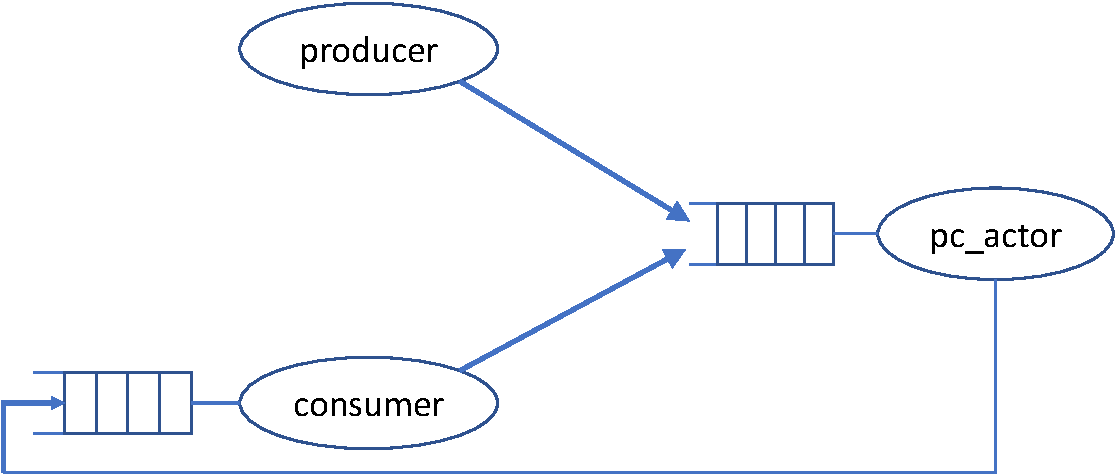
\includegraphics[width=4in]{figures/actor-crop.pdf}
\end{center}
\caption{Depiction of three actors.  The producer does not receive messages.}
\label{fig:actorpic}
\end{figure}

\begin{figure}
\begin{code}
\harmonysource{counter}
\end{code}
\caption{\harmonylink{code/counter.hny} An illustration of the actor approach.}
\label{fig:actor}
\end{figure}

Some programming languages favor a different way of implementing
synchronization using so-called \emph{actors}~\cite{HBS73,Agha86}.  Actors are
threads that have only private memory and communicate through
\emph{message passing}.
See \autoref{fig:actorpic} for an illustration.
Given that there is no shared memory in the actor model (other than the message
queues, which have built-in synchronization), there is no need
for critical sections.  Instead, some sequential thread owns a particular
piece of data and other threads access it by sending request messages
to the thread and optionally waiting for response messages.  Each thread
handles one message at a time, serializing all access to the data it owns.
As message queues are FIFO (First-In-First-Out), starvation is prevented.

The actor synchronization model is popular in a variety of programming
languages, including Erlang and Scala.  Actor support is also available
through popular libraries such as Akka, which is available for various
programming languages.  In Python, Java, and C/C++,
actors can be easily emulated using threads and \emph{synchronized queues}
\index{synchronized queue}%
(aka \emph{blocking queues})
\index{blocking queue}%
for messaging.
Each thread would have one such queue for receiving messages.
Dequeuing from an empty synchronized queue blocks the thread until
another thread enqueues a message on the queue.

The \texttt{synch} library supports a synchronized message queue,
similar to the \texttt{Queue} object in Python.
Its interface is as follows:
\begin{itemize}
\item \texttt{Queue()} returns a new message queue;
\item \texttt{put}($q$, \textit{item}) adds \textit{item} to the queue pointed to by $q$;
\item \texttt{get}($q$) waits for and returns an item on the queue pointed to by $q$.
\end{itemize}

For those familiar with counting semaphores: note that a \texttt{Queue}
behaves much like a zero-initialized counting semaphore.
\texttt{put} is much like \texttt{V}, except that it is accompanied by data.
\texttt{get} is much like \texttt{P}, except that it also returns data.
Thus, synchronized queues can be considered a generalization of
counting semaphores.

\autoref{fig:actor} illustrates the actor approach.
There are three client threads that each want to be assigned
a unique identifier from the set $\{ 0, 1, 2 \}$.
Normally one would use a shared 0-initialized counter and a lock.
Each client would acquire the lock, get the value of the counter
and increment it, and release the lock.
Instead, in the actor approach the counter is managed by a
separate server thread.
The server never terminates, so it is spawned with the keyword
\textbf{eternal} to suppress non-terminating state warnings.
Each client sends a request to the server, consisting in this case
of simply the queue to which the server must send the response.
The server maintains a local, zero-initialized counter variable.
Upon receiving a request, it returns a response with the value of
the counter and increments the counter.  No lock is required.
The code is tested using the \textit{done} array.

This illustration is an example of the \emph{client/server} model.
Here a single actor implements some service, and clients send request
messages and receive response messages.  The model is particularly
popular in distributed systems, where each actor runs on a separate
machine and the queues are message channels.  For example, the server
can be a web server, and its clients are web browsers.

\section*{Exercises}
\begin{problems}
\item Actors and message queues are good for building pipelines.
Develop a pipeline that computes Mersenne primes (primes that are one less
than a power of two).  Write four actors:
\begin{enumerate}
\item an actor that generates a sequence of integers 1 through \texttt{N};
\item an actor that receives integers and forwards only those that are prime;
\item an actor that receives integers and forwards only those that are one
less than a power of two;
\item an actor that receives integers but otherwise ignores them.
\end{enumerate}
Configure two versions of the pipeline, one that first checks if a number
is prime and then if it is one less than a power of two, the other
in the opposite order.  Which do you think is better?
\end{problems}

\chapter{Barrier Synchronization}
\label{ch:barrier}
\index{barrier synchronization}%

\glsadd{barrier synchronization}%

\begin{figure}
\begin{code}
\harmonysource{qbarrier}
\end{code}
\caption{\harmonylink{code/qbarrier.hny} Barrier synchronization with queues.}
\label{fig:barrier}
\end{figure}

Barrier synchronization is a problem that comes up in high-performance
parallel computing.
It is used, among others, for scalable simulation.
A barrier is almost the opposite of a critical section:
the intention is to get a group of threads to run some code at the
same time, instead of having them execute it one at a time.
More precisely, with barrier synchronization the threads execute in rounds.
Between each round there is a so-called \emph{barrier} where threads wait
until all threads have completed the previous round, before they start the
next one.
For example, in an iterative matrix algorithm, the matrix may be
cut up into fragments.  During a round, the threads run concurrently,
one for each fragment.  The next round is not allowed to start
until all threads have completed processing their fragment.

\begin{comment}
\begin{figure}
\begin{center}
\includegraphics[width=\textwidth]{figures/barrier-crop.pdf}
\end{center}
\caption{High-level state diagram specification of barrier synchronization
with three threads and two rounds.  The three numbers specify how many
rounds each thread has completed.}
\label{fig:barrierdiagram}
\end{figure}

\autoref{fig:barrierdiagram} shows a high-level depiction of barrier synchronization
with three and threads.  Initially all threads are in round~0.  Then each thread
can start and finish the round.  However, none of the threads can
progress to the next round until all threads have finished the
current round.
\end{comment}

Blocking queues work well for implementing barrier synchronization.
\autoref{fig:barrier} shows an example.  There is a queue
for each of the \texttt{N} threads.
Before thread $i$ enters a round, it first sends a message to every
other thread and then waits until it receives a message from
every other thread.
In this simple case, each message contains \texttt{None}, but in practice useful
information may be exchanged between the threads.

The \textit{round} array is kept to check the correctness of this
approach.  Each thread increments its entry every time it enters
a round.  If the algorithm is correct, it can never be that two threads
are more than one round apart.

\begin{figure}
\begin{code}
\harmonysource{barrier}
\end{code}
\caption{\harmonylink{code/barrier.hny} Generalized barrier synchronization.}
\label{fig:genbarrier}
\end{figure}

\begin{figure}
\begin{code}
\harmonysource{barriertest}
\end{code}
\caption{\harmonylink{code/barriertest.hny} Test program for \autoref{fig:genbarrier}.}
\label{fig:barriertest}
\end{figure}

More generally, barrier synchronization can be abstracted as follows.
We want to create a \texttt{Barrier}$(n)$ object, with operations
\texttt{enter()} and \texttt{exit()}.  It is helpful to use
a roller coaster car with $n$ seats as a metaphor:
\begin{itemize}
\item the car cannot contain more than $n$ people;
\item the car won't take off until $n$ people are in the car;
\item no new people can enter the car until all $n$ people have left it.
\end{itemize}
Notice there are two different waiting conditions:
\begin{enumerate}
\item waiting for the car to empty out;
\item waiting for the car to fill up.
\end{enumerate}

But this poses a complication.  Suppose, for example, that there are two
seats in the car, and there is one person in the car.  Does that mean that
the car is not yet full, or not yet empty?  We have to distinguish
those situations.  To this end, it is useful to think of the car as going through
$2 \cdot n$ stages:
\begin{itemize}
\item[] Stage 0: the car is empty;
\item[] Stage $1 ... n-1$: the car is filling up;
\item[] Stage $n$: the car is full;
\item[] Stage $n+1 ... 2n - 1$: the car is emptying out.
\end{itemize}

\autoref{fig:genbarrier} shows code that implements barrier synchronization
using these stages.
Method~\texttt{enter}() has two \texttt{wait} loops, one for each
waiting condition.
This is sometimes called \emph{double turnstile}.
Each loop uses a different condition variable.
The first loop waits until the car has emptied out, while
the second waits for the car to fill up.
\autoref{fig:barriertest} is a test program.  The threads check
that all threads within the barrier are in the same round.

\section*{Exercises}
\begin{problems}
\item Implement barrier synchronization for \texttt{N} threads
with just three binary semaphores.  Busy waiting is not allowed.
Can you implement barrier synchronization with two binary semaphores?
(As always, the Little Book of Semaphores~\cite{Downey09} is a good resource
for solving synchronization problems with semaphores.
Look for the \emph{double turnstile}
\index{double turnstile}%
solution.)
\item Imagine a pool hall with \texttt{N} tables.  A table is \emph{full}
from the time there are two players until both players have left.
When someone arrives, they can join a table that is not full, preferably
one that has a player ready to start playing.
Implement a simulation of such a pool hall.
\end{problems}

\chapter{Interrupts}
\label{ch:interrupts}
\index{interrupt}

\begin{figure}
\begin{code}
\harmonysource{trap}
\end{code}
\caption{\harmonylink{code/trap.hny} How to use \textbf{trap}.}
\label{fig:trap}
\end{figure}

\begin{figure}
\begin{code}
\harmonysource{trap2}
\end{code}
\caption{\harmonylink{code/trap2.hny} A race condition with interrupts.}
\label{fig:trap2}
\end{figure}

\begin{figure}
\begin{code}
\harmonysource{trap3}
\end{code}
\caption{\harmonylink{code/trap3.hny} Locks do not work with interrupts.}
\label{fig:trap3}
\end{figure}

\begin{figure}
\begin{code}
\harmonysource{trap4}
\end{code}
\caption{\harmonylink{code/trap4.hny} Disabling and enabling interrupts.}
\label{fig:trap4}
\end{figure}

Threads can be \emph{interrupted}.  An interrupt is a notification
of some event such as a keystroke, a timer expiring, the reception
of a network packet, the completion of a disk operation, and so on.
We distinguish \emph{interrupts} and \emph{exceptions}.  An exception
is caused by the thread executing an invalid machine instruction
such as divide-by-zero.  An interrupt is caused by some peripheral
device and can be handled in Harmony.  In other words: an interrupt
is a notification, while an exception is an error.  \index{exception}

Harmony allows modeling interrupts using the \texttt{trap} statement:
\begin{code}
\textbf{trap} \textit{handler} \textit{argument}
\end{code}
invokes \textit{handler argument} at some later, unspecified time.
Thus you can think of \textbf{trap} as setting a timer.
Only one of these asynchronous events can be outstanding at a time;
a new call to \textbf{trap} overwrites any outstanding one.
\autoref{fig:trap} gives an example of how \textbf{trap} might be used.
Here, the \textit{main}() thread loops until the interrupt has occurred and
the \textit{done} flag has been set.

But now consider \autoref{fig:trap2}.  The difference with \autoref{fig:trap} is
that both the \textit{main}() and \textit{handler}() methods increment \textit{count}.
This is not unlike the example we gave in \autoref{fig:inc}, except that only a single
thread is involved now.  And, indeed, it suffers from a similar race condition; run
it through Harmony to see for yourself.  If the interrupt occurs after \textit{main}()
reads \textit{count} (and thus still has value 0) but before \textit{main()} writes the
updated value~1, then the interrupt handler will also read value~0 and write value~1.
We say that the code in \autoref{fig:trap2} is not \textit{interrupt-safe} (as opposed
to not being \textit{thread-safe}).
\index{interrupt-safety}

You would be excused if you wanted to solve the problem using locks, similar to
\autoref{fig:incfixed}.  \autoref{fig:trap3} shows how one might go about this.
But locks are intended to solve synchronization issues between multiple threads.
If you run the code through Harmony, you will find that the code may not terminate.
The issue is that a thread can only acquire a lock once.  If the interrupt happens
after \textit{main}() acquires the lock but before \textit{main}() releases it, the
\textit{handler}() method will block trying to acquire the lock, even though
it is being acquired by the same thread that already holds the lock.

Instead, the way one fixes interrupt-safety issues is through disabling interrupts
temporarily.  In Harmony, this can be done by setting the \textit{interrupt level}
of a thread to \texttt{True} using the \textbf{setintlevel} interface.
\autoref{fig:trap4} illustrates how this is done.
Note that it is not necessary to change the interrupt level during servicing an
interrupt, because it is automatically set to \texttt{True} upon entry to the interrupt
handler and restored to \texttt{False} upon exit.
It is important that the \textit{main}() code re-enables interrupts after incrementing
\textit{count}.  What would happen if \textit{main}() left interrupts disabled?

\textbf{setintlevel}(\textit{il}) sets the interrupt level to \textit{il} and returns
the prior interrupt level.  Returning the old level is handy when writing interrupt-safe
methods that can be called from ordinary code as well as from an interrupt handler.
\autoref{fig:trap5} shows how one might write a interrupt-safe method
to increment the counter.

\begin{figure}
\begin{code}
\harmonysource{trap5}
\end{code}
\caption{\harmonylink{code/trap5.hny} Example of an interrupt-safe method.}
\label{fig:trap5}
\end{figure}

\begin{figure}
\begin{code}
\harmonysource{trap6}
\end{code}
\caption{\harmonylink{code/trap6.hny} Code that is both interrupt-safe and thread-safe.}
\label{fig:trap6}
\end{figure}

It will often be necessary to write code that is both interrupt-safe \emph{and}
thread-safe.  As you might expect, this involves both managing locks and
interrupt levels.
To increment \textit{count}, the interrupt level must be \textit{True} and
\textit{countlock} must be held.
\autoref{fig:trap6} gives an example of how this might be done.
One important rule to remember is that a thread should disable interrupts \emph{before}
attempting to acquire a lock.

Try moving \texttt{lock}() to the beginning of the \texttt{increment} method
and \texttt{unlock}() to the end of \texttt{increment} and see what happens.
While Harmony will only report one faulty run, this incorrect code can lead to
the assertion failing as well as threads getting blocked indefinitely.

(Another option is to use synchronization techniques that do not use locks.
See \autoref{ch:nonblocking} for more information.)

There is another important rule to keep in mind.  Just like locks should never be held
for long, interrupts should never be disabled for long.  With locks the issue is to
maximize concurrent performance.  For interrupts the issue is fast response to
asynchronous events.  Because interrupts may be disabled only briefly, interrupt
handlers must run quickly and cannot wait for other events.  It is ok to invoke
non-blocking synchronization calls such as \texttt{notify}, but calls such as
\texttt{acquire} and \texttt{wait} should only be used if it is certain that they will not
block for long.  Informally, interrupt handlers can be
\emph{producers} but not \emph{consumers} of synchronization events.

\section*{Exercises}
\begin{problems}
\item The \texttt{put} method you implemented in \autoref{ex:bbmesa} cannot be used
in interrupt handlers for two reasons: (1) it is not interrupt-safe, and (2)
it may block for a long time if the buffer is full.  Yet, it would be useful if,
say, a keyboard interrupt handler could place an event on a shared queue.
Implement a new method \texttt{i\_put}(\textit{item}) that does not
block.  Instead, it should return \texttt{False} if the buffer is full and \texttt{True}
if the item was successfully enqueued.
The method also needs to be interrupt-safe.
\end{problems}

\chapter{Non-Blocking Synchronization}
\label{ch:nonblocking}
\index{non-blocking synchronization}%

\glsadd{non-blocking synchronization}%

\begin{figure}
\begin{code}
\harmonysource{hw}
\end{code}
\caption{\harmonylink{code/hw.hny} Non-blocking queue.}
\label{fig:hw}
\end{figure}

So far, we have concentrated on critical sections to synchronize multiple
threads.  Certainly, preventing multiple threads from accessing
certain code at the same time simplifies how to think about synchronization.
However, it can lead to starvation.  Even in the absence of starvation,
if some thread is slow for some reason while being in the critical section,
the other threads have to wait for it to finish executing the critical section.
Also, using synchronization primitives in interrupt handlers is tricky
to get right (\autoref{ch:interrupts}) and might be too slow.
In this chapter, we will have a look at how one can develop concurrent
code in which threads do not have to wait for other threads (or interrupt
handlers) to complete their ongoing operations.

As an example, we will revisit the producer/consumer problem.
The code in \autoref{fig:hw} is based on code developed by Herlihy and
Wing~\cite{HW87}.
The code is a ``proof of existence'' for non-blocking synchronization; it
is not necessarily practical.
There are two variables.  \textit{items} is an unbounded array with each
entry initialized to \texttt{None}.  \textit{back} is an index into the
array and points to the next slot where a new value is inserted.
The code uses two atomic operations:
\begin{itemize}
\item \texttt{inc}($p$): atomically increments \texttt{!}$p$ and returns
the old value;
\item \texttt{exch}($p$): sets \texttt{!}$p$ to \texttt{None} and returns
the old value.
\end{itemize}

Method \texttt{produce}(\textit{item}) uses \texttt{inc}(?\textit{back})
to allocate
the next available slot in the \textit{items} array.
It stores the item as a singleton tuple.
Method \texttt{consume()} repeatedly scans the array, up to the
\textit{back} index, trying to find an item to return.
To check an entry, it uses \texttt{exch()}
to atomically remove an item from a slot if there is one.
This way, if two or more threads attempt to extract an item from
the same slot, at most one will succeed.

There is no critical section.  If one thread is executing instructions
very slowly, this does not negatively impact the other threads, as it
would with solutions based on critical sections.
On the contrary, it helps them because it creates less contention.
Unfortunately, the solution is not practical for the following reasons:
\begin{itemize}
\item The \textit{items} array must be of infinite size if an unbounded number
of items may be produced;
\item Each slot in the array is only used once, which is inefficient;
\item the \texttt{inc} and \texttt{exch} atomic operations are not
universally available on existing processors.
\end{itemize}
However, in the literature you can find examples of practical
non-blocking (aka \emph{wait-free})
\index{wait-free synchronization}%
synchronization algorithms.
% TODO~\cite{}.

\begin{comment}
There are also various algorithms where read-only access is wait-free
but updates do require a lock---these are useful in situations where
most accesses are read-only and the performance of updates is less
critical. %~\cite{}.
\end{comment}

\section*{Exercises}
\begin{problems}
\item A \emph{seqlock}
\index{seqlock}%
consists of a lock and a version number.
An update operation acquires the lock, increments the version number, makes the
changes to the data structure, and then releases the lock.  A read-only operation
does not use the lock.  Instead, it retrieves the version number,
reads the data structure, and then checks if the
version number has changed.  If so, the read-only operation is retried.
Use a seqlock to implement a bank much like \autoref{ex:bank}, with
one seqlock for the entire bank (i.e., no locks on individual accounts).
Method \texttt{transfer} is an update operation; method \texttt{total} is a
read-only operation.  Explain how a seqlock can lead to starvation.
\end{problems}

\chapter{Alternating Bit Protocol}
\label{ch:abp}
\index{alternating bit protocol}%
\index{protocol}%
\index{distributed system}%

\begin{figure}
\begin{code}
\harmonysource{abp}
\end{code}
\caption{\harmonylink{code/abp.hny} Alternating Bit Protocol.}
\label{fig:abp}
\end{figure}

\begin{figure}
\begin{code}
\harmonysource{abptest}
\end{code}
\caption{\harmonylink{code/abptest.hny} Test code for alternating bit protocol.}
\label{fig:abptest}
\end{figure}

A
\emph{distributed system}
\index{distributed system}%
is a concurrent system in which a collection
of threads communicate by message passing, much the same as
in the actor model.
The most important difference between distributed and concurrent
systems is that the former takes \emph{failures}
\index{failure}%
into account,
including failures of threads and failures of shared memory.
In this chapter, we will consider two actors, Alice and Bob.
Alice wants to send a sequence of application messages to Bob,
but the underlying network may lose messages.
\index{network}%
The network does not re-order messages: when sending messages
$m_1$ and $m_2$ in that order, then if both messages are received,
$m_1$ is received before $m_2$.
Also, the network does not create messages out of nothing: if
message $m$ is received, then message $m$ was sent.

It is useful to create an abstract network that reliably sends messages
between threads, much like the FIFO queue in the \texttt{synch} module.
For this, we need a network protocol that Alice and Bob can run.
In particular, it has to be the case that if Alice sends application
messages $m_1, ..., m_n$ in that order, then if Bob receives an
application message
$m$, then $m = m_i$ for some $i$ and Bob will already have received
application messages $m_1, ..., m_i$ (safety).
Also, if the network is fair and Alice sends application message
$m$, then eventually Bob should deliver $m$ (liveness).

The \emph{Alternating Bit Protocol} is suitable for our purposes.
We assume that there are two unreliable network channels: one from Alice
to Bob and one from Bob to Alice.
Alice and Bob each maintain a zero-initialized
\emph{sequence number},
\index{sequence number}%
\textit{s\_seq} and \textit{r\_seq} resp.
Alice sends a network message to Bob containing an
application message as \emph{payload} and Alice's sequence number
as \emph{header}.
When Bob receives such a network message, Bob returns an
\emph{acknowledgment}
\index{acknowledgment}%
to Alice, which is a network message
containing the same sequence number as in the message that Bob received.

In the protocol, Alice keeps sending the same network message until she
receives an acknowledgment with the same sequence number.
This is called \emph{retransmission}.
\index{retransmission}%
When she receives the desired sequence number, Alice increments her sequence number.
She is now ready to send the next message she wants to send to Bob.
Bob, on the other hand, waits until he receives a message matching
Bob's sequence number.  If so, Bob \emph{delivers} the payload in the
message and increments his sequence number.
Because of the network properties,  a one-bit sequence number suffices.

We can model each
channel as a variable that either contains a network message or nothing
(we use \texttt{()} in the model).  Let \textit{s\_chan} be the channel
from Alice to Bob and \textit{r\_chan} the channel from Bob to Alice.
\texttt{net\_send}(\textit{pchan}, $m$, \textit{reliable}) models sending
a message $m$ to
\texttt{!}\textit{pchan}, where \textit{pchan} is either ?\textit{s\_chan}
or ?\textit{r\_chan}.
The method places either $m$ (to model a successful send)
or \texttt{()} (to model loss) in \texttt{!}\textit{pchan}.
The use of the \textit{reliable} flag will be explained later.
\texttt{net\_recv}(\textit{pchan}) models checking \texttt{!pchan} for
the next message.

Method \texttt{app\_send}($m$) retransmits $m$ until
an acknowledgment is received.
Method \texttt{app\_recv}(\textit{reliable}) returns the next successfully received
message.
\autoref{fig:abptest} shows how the methods may be used to send and receive
a stream of \texttt{NMSGS} messages reliably.
It has to be bounded, because model checking requires a finite model.

Only the last invocation of \texttt{app\_recv}(\textit{reliable}) is invoked with
\textit{reliable} == \texttt{True}.  It causes the last acknowledgment to be sent
reliably.  It allows the receiver (Bob) to stop, as well as the sender (Alice)
once the last acknowledgment has been received.
Without something like this, either the sender may be left hanging waiting
for the last acknowledgment, or the receiver waiting for the last message.

\section*{Exercises}
\begin{problems}
\item \autoref{ch:actor} explored the \emph{client/server model}.  It is popular
in distributed systems as well.
Develop a protocol for a single client and server using the same network
model as for the ABP protocol.
Hint: the response to a request can contain the same sequence number as the
request.
\item Generalize the solution in the previous exercise to multiple clients.
Each client is uniquely identified.  You may either use separate channel pairs
for each client, or solve the problem using a single pair of channels.
\end{problems}

\chapter{Leader Election}
\label{ch:leader}

\begin{figure}
\begin{code}
\harmonysource{leader}
\end{code}
\caption{\harmonylink{code/leader.hny} A leader election protocol on a ring.}
\label{fig:leader}
\end{figure}

Leader election is the problem of electing a unique leader in a
network of processors.  Typically this is challenging because the
processors have only limited information.  In the version that we
present, each processor has a unique identifier.  The processors
are organized in a ring, but each processor only knows its own
identifier and the identifier of its successor on the ring.  Having
already looked into the problem of how to make the network reliable,
we assume here that each processor can reliably send messages to
its successor.

The protocol that we present elects as leader the processor with the
highest identifier~\cite{CR79} and works in two phases: in the first
phase, each processor sends its identifier to its successor.  When
a processor receives an identifier that is larger than its own
identifier, it forward that to its successor as well.  If a processor
receives its own identifier, it discovers that it is the leader.  That
processor then starts the second phase by sending a message around the
ring notifying the other processors of the leader's identifier.

\autoref{fig:leader} describes the protocol and its test cases in Harmony.
To test the protocol, the code first generates an identifier for each
processor, chosen non-deterministically from a set of \texttt{NIDS}
identifiers.  It also keeps track in the variable \textit{leader} of
what the highest identifier is so it can later be checked.

The network is modeled simply as a set of messages.
The \texttt{send} method atomically adds a message to this set.
Messages are tuples with three fields:
(\textit{dst}, \textit{id}, \textit{found}).
\textit{dst} is the identifier of the destination processor;
\textit{id} is the identifier that is being forwarded; and
\textit{found} is a boolean indicating the second phase of the protocol.
The \texttt{receive}(\textit{self}) method looks for all messages
destined for the processor with identifier \textit{self}.

Method \texttt{processor}(\textit{self}, \textit{succ}) is the
code for a processor with identifier \textit{self} and successor
\textit{succ}.
It starts simply by sending its own identifier to its successor.
The processor then loops until it discovers the identifier of the
leader in the second phase of the protocol.
A processor waits for a message using the Harmony \textbf{select} statement.
This statement takes the form \textbf{select} $v$ \textbf{in} $s$: \emph{statement block}
where $s$ is a set and $v$ is variable that is bound to an element of $s$.
The properties of the \textbf{select} statement are as follows:
\begin{itemize}
\item it waits until $s$ is non-empty;
\item it is executed atomically;
\item $v$ is selected non-deterministically, like in the \texttt{choose} operator.
\end{itemize}
\index{select statement}%

If a processor receives its own identifier, it knows its the leader.
The Harmony code checks this using an assertion.
In real code the processor could not do this as it does not know
the identifier of the leader, but assertions are only there to check
correctness.
The processor then sends a message to its successor that the leader
has been found.
If the processor receives an identifier higher than its own, the
processor knows that it cannot be the leader.
In that case, it simply forwards the message.
A processor stops when it receives a message that indicates that
the leader has been identified.

Note that there is a lot of non-determinism in the specification, leading
to a lot of executions that must be checked.
First, every possible permutation of identifiers for the processors
is tried.  When there are multiple messages to receive by a processor,
every possible order is tried (including receiving the same message
multiple times).  Fortunately, the \texttt{select} statement is executed
atomically, otherwise the body of the statement could lead to additional
thread interleavings.  Because in practice the different processors do
not share memory, it is not necessary to check those interleavings.

\section*{Exercises}
\begin{problems}
\item Check if the code finds a unique leader if identifiers are not unique.
\item Messages are added atomically to the network.  Is this necessary?
What happens if you remove the \textbf{atomic} keyword?  Explain what happens.
\end{problems}

\chapter{Transactions and Two Phase Commit}
\label{ch:2pc}

\begin{figure}
\begin{code}
\harmonysource{2pc1}
\end{code}
\caption{\harmonylink{code/2pc.hny} Two Phase Commit protocol: code for banks.}
\label{fig:2pc1}
\end{figure}

\begin{figure}
\begin{code}
\harmonysource{2pc2}
\end{code}
\caption{\harmonylink{code/2pc.hny} Two Phase Commit protocol: code for transaction coordinators.}
\label{fig:2pc2}
\end{figure}

Modern databases support multiple clients concurrently accessing the data.
They store data on disk, but we will ignore that in this book.
(If you want to model a disk, this is probably best done as a separate
thread.)
The complication we address here is that databases may be \emph{sharded},
where different parts of the data are stored on different servers.
The different servers may even be under different
authoritive domains, such as multiple banks maintaining the accounts of their
clients.

In database terminology, a \emph{transaction} is an operation on a database.
The operation can be quite complex, and the execution of a transaction
should have at least the following two properties:
\begin{itemize}
\item \emph{all-or-nothing}: a transaction should either complete, or it should
be a no-op.  It should never partially execute and then give up because of
some kind of error or something.  Database
people call this \emph{atomicity}, but it is not the same kind of atomicity that
we have been discussing in this book.
\item \emph{serialized}: any two concurrent transactions should appear to
execute in some order.  Database people call this \emph{isolation}: one transaction
should not be able to witness the intermediate state of another transaction
in execution.
\end{itemize}

We will use as an example a distributed database that maintains accounts.
For simplicity we will model this as a collection of banks, each maintaining a
single account.  There are two kinds of transactions: \emph{transfer}
(similar to \autoref{ex:bank}) and \emph{check}.  In this example, a transfer
is a transaction that moves some funds between two accounts.
A check is a transaction over all accounts and checks that the sum of the
balances across the accounts remains the same.

Executing such transactions must be done with care.  Consider what
would happen if transactions are not all-or-nothing or are not
serialized.  A transfer consists of two operations: withdrawing
funds from one account and depositing the same amount of funds in
the other.  These two operations can be done concurrently, but if
the withdrawal fails (for example, because there are not sufficient
funds in the source account) then the whole transaction should fail
and become a no-op.  Even if this is not the case, a concurrent
check transaction may accidentally witness a state in which either
the withdrawal or the deposit happened, but not both.  And matters
get more complicated with multiple concurrent transfers.

The Two-Phase Commit protocol~\cite{Gray78} is a protocol that can be
used to implement transactions across multiple database servers---banks
in this case.
Each transaction has a \emph{coordinator} that sends a \texttt{PREPARE}
message to each of the servers involved in the transaction, asking them
to prepare to commit to their part in a particular transaction.
A server can either respond with
\texttt{YES} if it is ready to commit and will avoid doing anything
that might jeopardize this (like committing a conflicting transaction),
or with \texttt{NO} if it does not want to participate in the transaction.
If all servers respond with \texttt{YES}, then the coordinator can
decide to \emph{commit} the transaction.  Otherwise the coordinator
must decide to \emph{abort} the transaction.  In the second phase, the
servers that responded with \texttt{YES} (if any) must be notified
to inform them of the coordinator's decision.

Different transactions can have different coordinators.  In our
implementation, each bank and each coordinator is a thread.
\autoref{fig:2pc1} shows the code for a bank.
The state of a bank consists of the following local variables:
\begin{itemize}
\item \textit{self}: the bank's identifier;
\item \textit{balance}: the current balance in the account;
\item \textit{status}: either contains () if the bank is not involved in an
ongoing transaction or contains the balance
just before the transaction started;
\item \textit{received}: the set of messages received and handled so far.
\end{itemize}

\noindent
Messages sent to a bank have the following dictionary format:
$\{ \mathtt{.dst}, \mathtt{.src}, \mathtt{.request}, \mathtt{.amount} \}$:
\begin{itemize}
\item \texttt{.dst}: identifier of the bank;
\item \texttt{.src}: identifier of the coordinator that sent the message;
\item \texttt{.request}: request type, which is either
\texttt{.withdraw}, \texttt{.deposit}, \texttt{.commit}, or \texttt{.abort};
\item \texttt{.amount}: amount to withdraw or deposit.
\end{itemize}

\noindent
A bank waits for a message destined to itself that it has not yet received.
In case of a withdrawal when the bank is idle and there are sufficient
funds, the bank saves the current balance in \textit{status} to indicate
an ongoing transaction and what its original balance was.
The bank then responds with a \texttt{.yes} message to the coordinator,
including the new balance.
Otherwise, the bank responds with a \texttt{.no} message.
Deposits are similar, except that it is not necessary to check for
sufficient funds.
In case of a \texttt{.commit} message, the bank changes its status
to (), indicating that there is no ongoing transaction.  In case of
a \texttt{.abort} message, the bank restores \textit{balance} first.

\autoref{fig:2pc2} contains the code for transfers and inquiries, as well
as tests.
The \texttt{receive()} method is used by coordinators in a \textbf{select}
statement to wait for a response from each bank involved in a transaction.
Argument \texttt{self} is the
identifier of the coordinator and \texttt{sources} is the set of banks.
It returns the empty set if there not yet responses from all banks.
Otherwise it returns a singleton set containing the set of responses,
one for each source.

The \texttt{transfer}() method contains the code for the transfer
transaction.  Argument \textit{self} is the identifier of the coordinator,
\textit{b1} is the source bank, \textit{b2} is the destination bank,
and \textit{amt} is the amount to transfer.
The coordinator sends a \texttt{PREPARE} message containing a
\texttt{.withdraw} request to \textit{b1} and a \texttt{PREPARE}
message containing a \texttt{.deposit} request to \textit{b2}.
It then waits for responses from each.  If both responses are
\texttt{.yes}, then it commits the transaction, otherwise it aborts
the transaction.

The \texttt{check}() method checks if the sum of the balances equals
\textit{total}, the sum of the initial balances.
The code is similar to \textit{transfer}, except that it always
aborts the transaction---there is no need to ever commit it.
As a code-saving hack: the balance inquiry is done by withdrawing \$0.

As for testing, the initial balances are picked arbitrarily between
0 and \texttt{MAX\_BALANCE} (and Harmony as always will try every
possible set of choices).
Each coordinator chooses whether to do a transfer or a check.  In
case of a transfer, it also chooses the source bank and the destination
bank.

While the protocol perhaps seems simple enough, there are a lot of
\textbf{if} statements in the code, making it hard to reason about
correctness.
Model checking is useful to see if there are corner
cases where the code does not work.
While confidence increases by
increasing the number of banks or the number of coordinators, doing so
quickly increases the number of possible states so that model checking
may become infeasible.

\section*{Exercises}
\begin{problems}
\item In \autoref{ex:bank} the code ran into a deadlock.  Can the code
in this chapter run into a deadlock?  Explain.
\item Transactions can fail for two reasons: a transfer transaction can
fail because of insufficient funds, but in general transaction can fail
if there is a conflict with another transaction.  The latter can be
fixed by retrying the transaction until it commits.  Implement this.
\item One way to reduce the number of conflicts between transactions
is to distinguish read and write operations.  Two read operations
(in our case, operations that withdraw \$0) do not conflict,
so a bank could have multiple ongoing read operations
for different transactions.  Implement this.
\item Two-phase commit can tolerate servers failing.  If a server does not
respond within some reasonable amount of time, the coordinator can abort
the transaction.  Implement this.
\end{problems}

\chapter{Replicated Atomic Read/Write Register}
\label{ch:abd}

\begin{figure}
\begin{code}
\harmonysource{abd}
\end{code}
\caption{\harmonylink{code/abd.hny} An implementation of a replicated atomic read/write register.}
\label{fig:abd}
\end{figure}

\begin{figure}
\begin{code}
\harmonysource{abdtest}
\end{code}
\caption{\harmonylink{code/abdtest.hny} Testing the code in \autoref{fig:abd}.}
\label{fig:abdtest}
\end{figure}

A \emph{register} is an object that you can read or write.  In a distributed
system, it can be useful to have shared registers.  A simple shared register
would be maintained by a server, and clients can read or write the
shared register by exchanging messages with the server.
We call two operations such that one does not finish before the other starts
\emph{concurrent}.
Since messages are delivered one at a time to the server,
concurrent operations on the shared register appear atomic.
In particular, we have the following three desirable properties:
\begin{enumerate}
\item All write operations are ordered;
\item A read operation returns either the last value written or the value of
a concurrent write operation.
\item If read operation $r_1$ finishes before read operation $r_2$ starts,
then $r_2$ cannot return a value that is older than the value returned
by $r_1$.
\end{enumerate}

\index{single point of failure}%
Unfortunately, however, the server is a \emph{single point of failure}:
if it fails, all its clients suffer.
We would therefore like to find a solution that can survive the crash
of a server.
In this chapter, we will \emph{replicate} the object: maintain multiple
copies.
One could, for example, imaging that clients write to all copies and read
from any single one.
While this solves the single-point-of-failure problem, we lose all the
nice properties above.  For one, it is not guaranteed that all servers
see all write operations in the same order.

\index{logical timestamp}%
We present a protocol here that is based on the work by
Hagit Attiya, Amotz Bar-Noy, and Danny Dolev~\cite{ABD95}.
In order to tolerate \texttt{N} failures,
it uses $\mathtt{N} = 2\mathtt{F} + 1$ servers.
Each server maintains not only the value of the object, but also a
\emph{logical timestamp} (see also \autoref{ch:testing}).
All write operation will be ordered by a unique timestamp.

\chapter{Distributed Consensus}
\label{ch:consensus}

\begin{figure}
\begin{code}
\harmonysource{bosco}
\end{code}
\caption{\harmonylink{code/bosco.hny} A crash-tolerant consensus protocol.}
\label{fig:bosco}
\end{figure}

Distributed consensus is the problem of having a collection of processors agree
on a single value over a network.
Without failures, this can be solved using leader election: first elect a leader, then have that leader decide a value.
But consensus often has to be done in adverse circumstances,
for example in the face of processor failures.
In Harmony, processors can be modeled by threads and there are a variety of ways in
which one can model a network using shared variables.
In this chapter, we will present a simple consensus algorithm that can tolerate
fewer than $1/3^{rd}$ of processors failing by crashing.

More precisely, we will
define a constant \texttt{F} that contains the maximum number of failures, and
assume there are $\texttt{N} = 3\texttt{F} + 1$ processors.
Each processor \emph{proposes} a value, which we assume here to be from the
set \{ 0, 1 \}.
By the usual definition of consensus, we want the following two properties:
\begin{enumerate}
\item \emph{Validity}: a processor can only decide a value that has been proposed;
\item \emph{Agreement}: if two processors decide, then they decide the same value.
\end{enumerate}
The consensus problem is surprisingly tricky to solve in the face of processor
failures and without making assumptions about how long it takes to send
and receive a message.

We will model the network as a bag (aka multiset) of messages.  The bag itself is
modeled in Harmony as a dictionary that maps unique elements in the bag to their
multiplicity.  So, for example, $\{ .\texttt{a}:1, .\texttt{b}:2 \}$ is the bag that consists of
one $.\texttt{a}$ and two copies of $.\texttt{b}$.
The \texttt{bag} module (\autoref{ap:bag}) contains a variety of handy functions on bags.
In this particular algorithm, all messages are broadcast to all processors, so they do
not require a destination address.

\autoref{fig:bosco} presents our algorithm.  Besides the network variable, it uses a
shared list of proposals and a shared set of decisions.  The invariants we want to maintain
on those variables is that $\textit{decisions} \subseteq \textit{proposals}$
and $|\textit{decisions}| \leq 1$.  Since the initial value of \textit{decisions} is
$\emptyset$, the invariants clearly hold initially.

The $\mathtt{N}$ processors go through a sequence of \emph{rounds} in which they wait for
$\texttt{N} - \texttt{F}$ messages, update their state based on the messages, and
broadcast messages containing their new state.
The reason that a processor waits for $\texttt{N} - \texttt{F}$ rather than \texttt{N}
messages is because of failures: up to $\texttt{F}$ processors may never send a message
and so it would be unwise to wait for all $\texttt{N}$.  You might be tempted to use
a timer and time out on waiting for a particular processor.  But how would you initialize
that timer?  While we will assume that the network is reliable, there is no guarantee
that messages arrive within a particular time.
We call a set of $\texttt{N} - \texttt{F}$ processors a \emph{quorum}.
A quorum must suffice for the algorithm to make progress.

The state of a processor consists
of its current round number and proposal.  Therefore, messages contain
a round number and a proposal. To start things, each processor first
broadcasts its initial round number (0) and proposal.
The number of rounds that are necessary to achieve consensus is not bounded.  But
Harmony can only check finite models, so there is a constant \texttt{NROUNDS} that
limits the number of rounds.  It may be that no decisions are made, but that does not
violate either Validity or Agreement.  We only check that \emph{if} decisions are
made, they satisfy Validity and Agreement.

In Line~21, a processor waits for $\texttt{N} - \texttt{F}$ messages using
the Harmony \textbf{select} statement.
Since Harmony has to check all possible executions of the protocol, the
\texttt{receive}(\textit{round}, $k$) method returns all \emph{subbags} of messages
for the given round that have size $k = \texttt{N} - \texttt{F}$.  The method uses a
dictionary comprehension to filter out all messages for the given \textit{round}
and then uses the \texttt{bag.combinations} method to find all combinations of size $k$.
The \textbf{select} statement waits until there is at least one such combination and
then chooses an element, which is bound to the \textit{quorum} variable.
The body of the \textbf{select} statement is then executed atomically.
This is usually how distributed algorithms are modeled, because they can only interact
through the network.  There is no need to interleave the different processes other
than when messages are delivered.  By executing the body atomically, a lot of
unnecessary interleavings are avoided and this reduces the state space that must
be explored by the model checker significantly.

The body of the \textbf{select} statement contains the core of the algorithm.
Note that $\texttt{N} - \texttt{F} = 2\texttt{F} + 1$, so that the number of
messages is guaranteed to be odd.  Also, because there are only 0 and 1 values, there
must exist a majority of zeroes or ones.  Variable \textit{count}[0] stores the number
of zeroes and \texttt{count}[1] stores the number of ones received in the round.
The rules of the algorithm are simple:
\begin{itemize}
\item update \textit{proposal} to be the majority value;
\item if the quorum is unanimous, decide the value.
\end{itemize}
After that, proceed with the next round.

One may wonder how failures can occur in this model.  They are not explicitly modeled, but
Harmony tries every possible execution, including executions in which some processors make
no execution steps unless there are no other processors that can run.  The way this algorithm
works, this includes executions in which $\texttt{N} - \texttt{F}$ processors terminate
before the remaining $\texttt{F}$ processors start executing.  To the first set of processors,
this is indistinguishable from executions in which the last set of processors have failed.

\section*{Exercises}
\begin{problems}
\item While Harmony checks that the Validity and Agreement properties
are not violated, it does not check that the algorithm ever decides.
Indeed, in unlucky executions the algorithm may never decide.  But
how would you check that there exist executions in which the algorithm
does decide?
\item The algorithm as given works in the face of crash failures.
A more challenging class to tolerate are \emph{arbitrary failures} in
which up to \texttt{F} processors may send arbitrary messages, including
conflicting messages to different peers (equivocation).
The algorithm can tolerate those failures if you use $\mathtt{N} = 5\mathtt{F} - 1$ processors instead of $\mathtt{N} = 3\mathtt{F} - 1$.  Check that.
\item In 1983, Michael Ben-Or presented a randomized algorithm that can
tolerate crash failures with
just $\mathtt{N} = 2\mathtt{F} - 1$ processors~\cite{BenOr83}.
Implement this algorithm.
\end{problems}

\chapter{Paxos}
\label{ch:paxos}

\begin{figure}
\begin{code}
\harmonysource{paxos1}
\end{code}
\caption{\harmonylink{code/paxos.hny} A version of the Paxos protocol, Part 1.}
\label{fig:paxos1}
\end{figure}

\begin{figure}
\begin{code}
\harmonysource{paxos2}
\end{code}
\caption{\harmonylink{code/paxos.hny} A version of the Paxos protocol, Part 2.}
\label{fig:paxos2}
\end{figure}

Paxos~\cite{Paxos} is the most well-known family of consensus protocols for
environments in which few or no assumptions are made about timing.
In this chapter we present a basic version of a Paxos protocol, one that is
\emph{single-decree} (only tries to make a single decision).
It uses two kinds of processors: \emph{leaders} and \emph{acceptors}.
In order to tolerate \texttt{F} crash failures, you need at least $\texttt{F}+1$ leaders
and $2\texttt{F} + 1$ acceptors, but leaders and acceptors can be colocated, so
in total only $2\texttt{F} + 1$ independently failing processors are needed.
Here we provide only a rudimentary introduction to Paxos; for more detailed
information refer to~\cite{Paxos}.

As in the consensus protocol of \autoref{ch:consensus}, Paxos uses rounds of messaging.
However, Paxos uses two kinds of rounds: ``Phase 1'' and ``Phase 2'' rounds.
The communication pattern is also different.  Rounds are identified by a so-called
\emph{ballot number} combined with the phase number.
Different leaders are in charge of different ballot numbers.
Leaders broadcast ``Type A''
messages to the acceptors, which respond point-to-point with ``Type B'' messages.

\autoref{fig:paxos1} and \autoref{fig:paxos2} contain the code for
this Paxos protocol.  Paxos is perhaps best understood starting
with the second phase.  At the end of the first phase the leader
broadcasts a \texttt{2.A} message (Phase 2, Type A) to the acceptors
containing the ballot number and a proposal and then waits for
$\texttt{N} - \texttt{F}$ matching \texttt{2.B} responses from the
acceptors.  If each response contains the ballot number and the
proposal, then the proposal is deemed decided.  But one or more of
the responses can contain a higher ballot number, in which case the
leader has to try again with an even higher ballot number.  This is
where the first phase comes in.

It is not possible that an acceptor responds with a smaller ballot
number.  This is because acceptors maintain two state variables.
One is \textit{ballot}, the highest ballot number they have seen.
Second is a variable called \textit{last\_accepted} that, if not
\texttt{None}, contains the last proposal the acceptor has
\emph{accepted} and the corresponding ballot number.  The acceptor
also contains a set \emph{received} that contains (ballot, phase)
tuples identifiying all rounds that the ballot has already participated
in.  An acceptor waits for a message for a round that is not in
\emph{received}.  If its ballot number is higher than what it has
seen before, the acceptor moves into that ballot.  If the phase is
2, then the acceptor accepts the proposal and remembers when it did
so by saving the (ballot, proposal) tuple in \textit{last\_accepted}.
In all cases, the acceptor responds with the current values of
\textit{ballot} and \textit{last\_accepted}.

In its first phase, a leader of a ballot must come up with a proposal that
cannot conflict with a proposal of an earlier ballot that may already
have been decided.  To this end, the leader broadcasts a \texttt{2.A}
message to the acceptors and awaits $\mathtt{N} - \mathtt{F}$ of their
\textit{last\_accepted}
values.  If all those acceptors responded with \texttt{None}, then the leader
is free to choose its own proposal.  Otherwise the leader updates
its proposal with the one corresponding to the highest ballot number.
The leader then moves on to the second round.

In the initialization, the \texttt{proposals} variable is initialized
to either $[\mathtt{False}, \mathtt{False}]$ or
to $[\mathtt{True}, \mathtt{False}]$ (in case $\texttt{NBALLOTS} = 2$).
The other combinations of \texttt{True} and \texttt{False} are symmetric,
so there is no need to run the model checker through those scenarios as
well, halving the running time.

\section*{Exercises}
\begin{problems}
\item Perhaps the trickiest detail of the algorithm is that, in Line~14
of \autoref{fig:paxos2}, the leader selects the proposal with the highest
ballot number it receives.  Replace the \texttt{max} operator in that statement
with \texttt{choose} and see if it finds a problem.  First try with
$\texttt{NBALLOTS} = 2$ and then with $\texttt{NBALLOTS} = 3$.
(Warning, the latter may take a long time.)  If it finds a problem,
analyze the output and see what went wrong.
\end{problems}

\bibliographystyle{alpha}
\bibliography{paper}

\appendix

\chapter{Value Types and Operators}
\label{ap:values}

\autoref{ch:harmonymachine} provides an introduction to Harmony values.
Below is a complete list of Harmony value types with examples:

\vspace{1em}
\begin{tabular}{|l|l|}
\hline
Boolean & \texttt{False}, \texttt{True} \\
\hline
Integer & \texttt{-inf, ..., -2, -1, 0, 1, 2, ..., inf} \\
\hline
Atom & \texttt{.example}, \texttt{.test1}, \texttt{.0x4A} \\
\hline
Program Counter & (method names are program counter constants) \\
\hline
Dictionary & \texttt{\{ .account: 12345, .valid: False \} } \\
\hline
Set & \texttt{\{\}, \{ 1, 2, 3 \}, \{ False, .id, 3 \} } \\
\hline
Address & \texttt{?lock, ?flags[2], None} \\
\hline
Context & (generated by \textbf{stop} expression) \\
\hline
\end{tabular}
\vspace{1em}

Tuples, lists, strings, and bags are all special cases of dictionaries.
Both tuples and lists map indexes (starting at 0) to Harmony values.
Their format is either \texttt{($e$, $e$, ..., $e$,)} or
\texttt{[$e$, $e$, ..., $e$,]}.
If the tuple or list has two or more elements, then the final comma
is optional.
A string is represented as a tuple of its characters.
Characters are one-character atoms, which can be expressed
in hexadecimal unicode using the syntax \texttt{.0xXX}.
A bag or multiset is a dictionary that maps a value to how many
times it occurs in the bag.

All Harmony values are ordered with respect to one another.  First they
are ordered by type according to the table above.
So, for example, \texttt{\texttt{True} < 0 < .xyz < \{ 0 \})}.
Within types, the following rules apply:

\begin{itemize}
\item \texttt{False < True};
\item integers are ordered in the natural way;
\item atoms are lexicographically ordered;
\item program counters are ordered by their integer values;
\item dictionaries are first converted into a list of ordered (key, value)
pairs.  Then two dictionaries are lexicographically ordered by this
representation;
\item a set is first converted into an ordered list, then lexicographically
ordered;
\item an address is a list of atoms.  \texttt{None} is the empty list of atoms.
Addresses are lexicographically ordered accordingly;
\item contexts (\autoref{app:context}) are ordered first by name, then by program counter, then by the remaining content.
\end{itemize}

Generic operators on Harmony values include:

\begin{center}
\begin{tabular}{|l|l|}
\hline
\texttt{$e$ == $e$} & equivalence \\
\hline
\texttt{$e$ != $e$} & inequivalence \\
\hline
\texttt{$e$ < $e$, $e$ <= $e$, $e$ > $e$, $e$ >= $e$} & comparison\\
\hline
\end{tabular}
\end{center}

\section{Boolean}

The Boolean type has only two possible values: \texttt{False} and
\texttt{True}.  Unlike in Python, in Harmony booleans are distinct
from integers, and in particular $\mathtt{False} < 0$.  In statements
and expressions where booleans are expected, it is not possible to
substibute values of other types.

Operations on booleans include:
\begin{center}
\begin{tabular}{|l|l|}
\hline
\texttt{$e$ and $e$ and ...} & conjuction \\
\hline
\texttt{$e$ or $e$ or ...} & disjunction \\
\hline
\texttt{$e$ => $e$, $e$ not => $e$} & implication \\
\hline
\texttt{not $e$} & negation \\
\hline
\texttt{$v$ if $e$ else $v'$} & $v$ or $v'$ depending on $e$ \\
\hline
\texttt{any $s$, all $s$} & disjunction / conjunction for set or list $s$ \\
\hline
\end{tabular}
\end{center}

\section{Integer}

The integer type supports any whole number, as well as $-\mathtt{inf}$
and $\mathtt{inf}$.  In the Python-based model checker, integers are
infinite precision.  In the C-based model checker, integers are implemented
by two's complement 61-bit words, and $-\mathtt{inf}$ is represented by
the minimal integer and $\mathtt{inf}$ is represented by the maximal integer.

Operations on integers include:

\begin{center}
\begin{tabular}{|l|l|}
\hline
\texttt{-$e$} & negation \\
\hline
\texttt{abs($e$)} & absolute value \\
\hline
\texttt{$e$ + $e$ + ...} & sum \\
\hline
\texttt{$e$ - $e$} & difference \\
\hline
\texttt{$e$ * $e$ * $e$ ...} & product \\
\hline
\texttt{$e$ / $e$, $e$ // $e$} & integer division \\
\hline
\texttt{$e$ \% $e$, $e$ mod $e$} & integer division remainder \\
\hline
\texttt{$e$ ** $e$} & power \\
\hline
\texttt{\string~$e$} & binary inversion \\
\hline
\texttt{$e$ \& $e$ \& ...} & binary and \\
\hline
\texttt{$e$ | $e$ | ...} & binary or \\
\hline
\texttt{$e$ \string^ $e$ \string^ ...} & binary exclusive or \\
\hline
\texttt{$e << e$} & binary shift left \\
\hline
\texttt{$e >> e$} & binary shift right \\
\hline
\texttt{$\{ e..e' \}$} & set of integers from $e$ to $e'$ inclusive \\
\hline
\end{tabular}
\end{center}

\section{Atom}

Atoms are essentially names and consist of one or more unicode characters.
If they do not contain special characters and do not start with a digit,
then an atom can be represented by a ``.'' followed by the characters.
For example, \texttt{.hello} is
a representation of the atom ``hello''.  A special character can be
represented by \texttt{.0xXX}, where \texttt{XX} is the hexidecimal
unicode for the character.
Atoms should not be confused with strings.
There are no special operations on atoms.
(In the future, operators may be introduced that convert between strings
and atoms.)

\section{Set}

In Harmony you can create a set of any collection of Harmony values.
Its syntax is \texttt{\{ $v_0, v_1, ...$ \}}.
Python users: note that in Harmony the empty set is denoted as $\{\}$.

The \texttt{set} module (\autoref{ap:set})
contains various convenient routines that operate on sets.
Native operations on sets include:

\begin{center}
\begin{tabular}{|l|l|}
\hline
\texttt{len $s$} & cardinality \\
\hline
\texttt{$s$ - $s$} & set difference \\
\hline
\texttt{$s$ \& $s$ \& ...} & intersection \\
\hline
\texttt{$s$ | $s$ | ...} & union \\
\hline
\texttt{$s$ \string^ $s$ \string^ ...} & inclusion/exclusion (elements in odd number of sets) \\
\hline
\texttt{choose $s$} & select an element (Harmony will try all) \\
\hline
\texttt{min $s$} & minimum element \\
\hline
\texttt{max $s$} & maximum element \\
\hline
\texttt{any $s$} & \texttt{True} if any value is \texttt{True} \\
\hline
\texttt{all $s$} & \texttt{True} if all values are \texttt{True} \\
\hline
\end{tabular}
\end{center}

Harmony also supports \emph{set comprehension}.  In its simplest form,
\texttt{\{ f($v$) for $v$ in $s$ \}} returns a set that is constructed
by applying \texttt{f} to all elements in $s$ (where $s$ is a set or
a list).
This is known as \emph{mapping}.  But set comprehension is much more
powerful and can include joining multiple sets (using nested for
loops) and filtering (using the \texttt{where} keyword).

For example:
\texttt{\{ $x$ + $y$ for $x$ in $s$ for $y$ in $s$ where $(x * y) == 4$ \}}
returns a set that is constructed by summing pairs of elements from $s$
that, when multiplied, have the value 4.

\section{Dictionary}

A dictionary maps a set of values (known as \emph{keys})
to another set of values.
The generic syntax of a dictionary is
$\{ k_0:v_0, k_1:v_1, ... \}$.
Different from Python, the empty dictionary is either $()$ or $[]$
(because $\{\}$ is the empty set in Harmony).
If there are duplicate keys in the list, then only the one with
the maximum value survives.
Therefore the order of the keys in the dictionary does not matter.

Dictionaries support comprehension.  The basic form is:
\texttt{\{ f($k$):g($k$) for $k$ in $s$ \}}.

There are various special cases of dictionaries,
including lists, tuples, strings,
and bags (multisets) that are individually described below.

Operations on dictionaries include the following:

\begin{center}
\begin{tabular}{|l|l|}
\hline
\texttt{$d~k$} & indexing \\
\hline
\texttt{len $d$} & the number of keys in $d$ \\
\hline
\texttt{keys $d$} & the set of keys in $d$ \\
\hline
\texttt{$v$ [not] in keys $d$} & check if $v$ is a \emph{key} in $d$ \\
\hline
\texttt{$v$ [not] in $d$} & check if $v$ is a \emph{value} in $d$ \\
\hline
\texttt{min $d$} & the minimum value in $d$ \\
\hline
\texttt{max $d$} & the maximum value in $d$ \\
\hline
\texttt{any $d$} & \texttt{True} if any value is \texttt{True} \\
\hline
\texttt{all $d$} & \texttt{True} if all values are \texttt{True} \\
\hline
\texttt{$d$ \& $d$ \& ...} & dictionary intersection \\
\hline
\texttt{$d$ | $d$ | ...} & dictionary union \\
\hline
\end{tabular}
\end{center}

Because in Harmony brackets are used for parsing purposes only,
you can write $d[k]$ (or $d(k)$) instead of $d~k$.
However, if $k$ is an atom, like \texttt{.id}, then you might
prefer the notation $k\mathtt{.id}$.

Python users beware: the Harmony \texttt{$v$ in $d$} operator checks
if there is some key $k$ such that $d[k] = v$.  In Python, the same
syntax checks if $v$ is a key in $d$.  The difference exists because
in Harmony a list is a special case of a dictionary.

Dictionary intersection and dictionary union are defined so that
they work well with bags.  With disjoint dictionaries, intersection
and union work as expected.  If there is a key in the intersection, then
dictionary intersection retains the minimum value while dictionary
union retains the maximum value.  Unlike Python, Harmony
dictionary intersection and union are commutative and associative.

\section{List or Tuple}

In Harmony, there is no distinction between a list or a tuple.
Both are a special case of dictionary.  In particular, a list of
$n$ values is represented by a dictionary that maps the integers
$0, ..., n-1$ to those values.  Hence, if $t$ is a list or tuple,
then the notation $t[0]$ returns the first element of the list.

You can denote a list by a sequence of values, each value terminated
by a comma.  As per usual, you can use brackets or parentheses
at your discretion.  For Python users, the important thing to note
is that a singleton list in Harmony must contain a comma.  For
example $[1,]$ is a list containing the value $1$, while $[1]$
is simply the value $1$.

The \texttt{list} module (\autoref{ap:list}) contains various
convenient routines that operate on lists or tuples.
Native operations on lists or tuples include the following:

\begin{center}
\begin{tabular}{|l|l|}
\hline
\texttt{$t~k$} & indexing \\
\hline
\texttt{$t$ + $t$ + ...} & concatenation \\
\hline
\texttt{$t$ * $n$} & $n$ copies of $t$ concatenated \\
\hline
\texttt{$v$ [not] in $t$} & check if $v$ is a \emph{value} in $t$ \\
\hline
\texttt{len $t$} & the length of $t$ \\
\hline
\texttt{min $t$} & the minimum value in $t$ \\
\hline
\texttt{max $t$} & the maximum value in $t$ \\
\hline
\texttt{any $t$} & \texttt{True} if any value is \texttt{True} \\
\hline
\texttt{all $t$} & \texttt{True} if all values are \texttt{True} \\
\hline
\texttt{$t$ \& $t$ \& ...} & pairwise list minimum \\
\hline
\texttt{$t$ | $t$ | ...} & pairwise list maximum \\
\hline
\end{tabular}
\end{center}

Lists and tuples support comprehension as well.
In their most basic form: \texttt{f($v$) for $v$ in $s$}.
For example, to check if any element in a list $t$ is even, you
can write:

\texttt{any($(x \% 2) == 0$ for $x$ in $t$)}.

\section{String}

In Harmony, a string is a list of single-character atoms.
The Python string notations mostly work in Harmony as well.
For example, \texttt{'abc'} is a three-character string
consisting of the atoms \texttt{.a}, \texttt{.b}, and
\texttt{.c}.
\texttt{"abc"} is the same three-character string.
Various special characters (including quotes, newlines, etc.)
can be \emph{escaped} using a backslash.
Multi-line strings can be terminated by triple quotes or
triple double-quotes.

Native operations on strings include the following:

\begin{center}
\begin{tabular}{|l|l|}
\hline
\texttt{$s~k$} & indexing \\
\hline
\texttt{$s$ + $s$ + ...} & concatenation \\
\hline
\texttt{$s$ * $n$} & $n$ copies of $s$ concatenated \\
\hline
\texttt{$c$ [not] in $s$} & check if $c$ (a one-character atom) is in $s$ \\
\hline
\texttt{len $s$} & the length of $s$ \\
\hline
\end{tabular}
\end{center}

\section{Bag or Multiset}

A bag is represented by a dictionary that maps each element to its
multiplicity, for example: \{ 10:2, 12:1 \}.
The \texttt{bag} module (\autoref{ap:bag}) contains various
convenient routines that operate on lists or tuples.
Native operations on bags include the following:

\begin{center}
\begin{tabular}{|l|l|}
\hline
\texttt{$v$ [not] in keys $b$} & check if $v$ is in $b$ \\
\hline
\texttt{$t$ \& $t$ \& ...} & bag intersection\\
\hline
\texttt{$t$ | $t$ | ...} & bag union \\
\hline
\end{tabular}
\end{center}

\section{Program Counter}

A program counter is an integer that can be used to index into Harmony
bytecode.  When you define a method, a lambda function, or a label,
you are creating a constant of the program counter type.

Operations on program counters include the following:
\begin{center}
\begin{tabular}{|l|l|}
\hline
\texttt{$m$ $a$} & invoke method with program counter $m$ and argument $a$\\
\hline
\texttt{atLabel $l$} & return a bag of (method, argument) pairs of threads executing at label $l$ \\
\hline
\end{tabular}
\end{center}

You can create lambda functions similarly to Python.  For example:
\texttt{lambda$(x,y)$:$x+y$}.

\section{Address}

In Harmony, each shared variable has an address, which is essentially
a list of Harmony values.
For example, the address of variable $d.\mathtt{v}[3]$ consists of the
list \texttt{.d}, \texttt{.v}, and 3.  The only way to construct an
address in Harmony is using the $?$ operator.
$?d.\mathtt{v}[3]$ returns the address of variable $d.\mathtt{v}[3]$.
An address can be dereferenced to return the value of the variable.
If $a$ is an address, then $!a$ returns the value.
Like C, Harmony supports the shorthand \texttt{$a$->v} for 
the expression \texttt{($!a$).v}.

\section{Context}

A context value captures the state of a thread.
A context is itself composed over various Harmony values.

\begin{comment}
Some of these values can be extracted.  In particular, if $c$
is a context, then:

\begin{center}
\begin{tabular}{|l|l|}
\hline
\texttt{\texttt{c}.name} & returns the name of the thread's main method \\
\hline
\texttt{\texttt{c}.entry} & returns the program counter of the thread's main method \\
\hline
\texttt{\texttt{c}.arg} & returns the argument value of the thread's main method \\
\hline
\texttt{\texttt{c}.this} & returns the thread-local state \\
\hline
\texttt{\texttt{c}.mode} & returns the \emph{mode} of the context \\
\hline
\end{tabular}
\end{center}

The possible modes of a context are as follows:

\begin{center}
\begin{tabular}{|l|l|}
\hline
\texttt{normal} & context of a executing thread \\
\hline
\texttt{stopped} & context of a stopped thread \\
\hline
\texttt{terminated} & context of a terminated thread \\
\hline
\texttt{failed} & context of a failed thread \\
\hline
\end{tabular}
\end{center}
\end{comment}

A thread can call \texttt{get\_context()} to retrieve its current
context.

\begin{comment}
Also, the function \texttt{contexts()} returns a
bag of all contexts (including terminated ones).
Both these functions should only be called in \texttt{atomic} mode
and used for checking invariants.
\end{comment}

\chapter{List of Statements}

Harmony currently supports the following statements (below, \texttt{S} is a list of statements):

\vspace{1em}
\begin{tabular}{|l|l|}
\hline
$e$ & $e$ is an expression\\
\hline
\textit{lv} = [lv =]... $e$ & \textit{lv} is an lvalue and $e$ is an expression\\
\hline
\textit{lv} \texttt{[op]=} $e$ & \texttt{op} is one of \texttt{+}, \texttt{-},
\texttt{*}, \texttt{/}, \texttt{//}, \texttt{\%},
\texttt{\&}, \texttt{|}, \texttt{\^},
\texttt{and}, \texttt{or}\\
\hline
\texttt{assert $b$ [, $e$]} & $b$ is a boolean.  Optionally report value of expression $e$\\
\hline
\texttt{atomic: S} & \texttt{S} a list of statements\\
\hline
\texttt{await $b$} & $b$ is a boolean\\
\hline
\texttt{const a = $e$} & \texttt{a} is a bounded variable, $e$ is a constant expression\\
\hline
\texttt{def m $a$: S} & \texttt{m} is an identifier, $a$ a bounded variable\\
\hline
\texttt{del} \textit{lv} & delete\\
\hline
\texttt{for $a[:b]$ in $e$ [where $c$]: S} & $a$ and $b$ are bounded variables, $e$ is a set or dictionary \\
\hline
\texttt{from m import ...} & \texttt{m} identifies a module \\
\hline
\texttt{go $c$ $e$} & $c$ is a context, $e$ is an expression \\
\hline
\texttt{if $b$: S else: S} & $b$ is a boolean, \texttt{S} is a list of statements\\
\hline
\texttt{import m, ...} & \texttt{m} identifies a module \\
\hline
\texttt{invariant e} & \texttt{e} is an invariant\\
\hline
\texttt{let $a$ = $e$ [let ...]: S} & $a$ is a bounded variable, $e$ is an expression\\
\hline
\texttt{pass} & do nothing\\
\hline
\texttt{select $a$ in $e$: S} & $a$ is a bounded variable, $e$ is a set,
                            \texttt{S} a list of statements\\
\hline
\texttt{sequential v, ...} & \texttt{v} has sequential consistency \\
\hline
\texttt{spawn [eternal] m $e$ [, $t$]} & \texttt{m} is a method,
$e$ is an expression, $t$ is the thread-local state \\
\hline
\texttt{trap m $e$} & \texttt{m} is a method and $e$ is an expression \\
\hline
\texttt{while $b$: S} & $b$ is a boolean, \texttt{S} a list of statements\\
\hline
\end{tabular}

\section{Single expression evaluation}

Any expression by itself can be used as a statement.  The most common
form of this is a function application, for example: \texttt{f}().
This statement evaluates \texttt{f}() but ignores its result.
It is equivalent to the assignment statement $\_ = \mathtt{f}()$.

\section{Assignment}

The statement $x = 3$ changes the state by assigning~3 to
variable $x$ (assuming~$x$ was not already~3).
$x$ may be a local variable or a shared variable.
The statement $x = y = 3$ first updates~$y$, then~$x$.
The statement $x[\mathtt{f}()] = y[\mathtt{g}()] = \mathtt{h}()$ first computes
the address of $x[\mathtt{f}()]$, then computes the address of
$y[\mathtt{g}()]$, then evaluates $\mathtt{h}()$, then assigns the resulting value to $y[\mathtt{g}()]$ (using its previously computed address), and finally assigns the same value to $x[\mathtt{f}()]$ (again using its previously computed address).
The statement $a,b = c$ assumes that $c$ is a tuple with two values.
It first evaluates the addresses of $a$ and $b$ and first assigns to
the latter and then the former.
If $c$ is not a tuple with two values, then Harmony will report an error.

Assigning to $\_$ evaluates the righthand side expression but is otherwise
a no-op.

The statement $x~+$$= 3$ loads $x$, adds 3, and then stores the
results in $x$.  In this case, it is equivalent to $x = x + 3$.
However, in general this is not so.  For example, $x[\mathtt{f}()]~+$$= 3$
only evaluates $\mathtt{f}()$ once.  Unlike Python, however,
$x~+$$= [3,]$ is equivalent to $x = x + [3,]$ in Harmony.
(In Python, the following two compound statements lead to different results
for $y$: $x = y = []; x~+$$= [3]$ and $x = y = []; x = x + [3]$.)

\section{\textbf{assert}}

The statement \textbf{assert $b$} evaluates $b$ and reports an error
if $b$ is false.  It should be considered a no-op---it is part of the
\emph{specification}, not part of the \emph{implementation} of the algorithm.
In particular, it specifies an invariant: whenever the program counter is
at the location where the \textbf{assert} statement is, then $b$ is
always true.

If $b$ is an expression, then it is evaluated atomically.
Moreover, the expression is not allowed to change the state.
If it does change the state, Harmony will report an error as well.

As in Python, you can specify an additional expression:
\textbf{assert $b$, $e$}.  The value of $e$ will be reported as part
of the error should $b$ evaluate to false.

\section{\textbf{atomic}}

The statement \textbf{atomic $S_1; S_2; ...$} evaluates statements
$S_1, S_2, ...$ atomically in that no other threads can run while
this atomic block is executing.  Typically an atomic block runs
to completion before any other thread can run.  The only exception
to this is if the atomic block executes a \textbf{stop} expression.
In this case, another thread can run.  When the original thread
is resumed (using a \textbf{go} statement), it is once again
atomically executing.

The \textbf{atomic} statement is useful for implementing synchronization
primitives such as test-and-set.  It is also useful for testing.
It is not a replacement for lock/unlock, and should not generally be used
for synchronization otherwise.  Lock/unlock does allow other
threads to run concurrently---just not in the same critical section.

\section{\textbf{await}}

The statement \textbf{await $b$} is equivalent to \textbf{while !$b$: pass}.
It is intended to improve readability of your code.

\section{\textbf{const}}

The expression \textbf{const} \texttt{N = 3} introduces a new constant
\texttt{N} with the value 3.  Evaluating \texttt{N} does not lead to
loading from a memory location.  The assignment can be overridden with
the \texttt{-c} flag: \texttt{harmony -cN=4} executes the model checker
with 4 assigned to \texttt{N} instead of 3.
Harmony also supports \textbf{const} \texttt{N, M = 3, 4}, which
assigns 3 to \texttt{N} and 4 to \texttt{M}.
Harmony has limited support for \emph{constant folding}.  For example,
\textbf{const} \texttt{N = 3 + 4} assigns value 7 to constant \texttt{N}.

\section{\textbf{def}}

The statement \textbf{def} \texttt{m} $a: S_1; S_2: ...$
defines a new program counter constant \texttt{m} referring to
a method that takes an argument $a$ and executes the statements
$S_1, S_2, ...$.  The argument $a$ can be a tuple pattern similar
to those used in \texttt{let} and \texttt{for} statements.
Examples include $()$, $(x,)$, $(x, y)$, and $(x, (y, z))$.
The given local variable names variable names are assigned
upon application.
It is allowed, but discouraged, to updates those local variables
in statements $S_1, S_2, ...$.
Each method has a predefined local variable
\textit{result}, initialized to \texttt{None},
that is returned by the method.  Harmony does
not support a \texttt{return} statement that \emph{breaks out}
of the code before executing the last statement.

\section{\textbf{del}}

The statement \textbf{del} $x$ removes variable $x$ from the
state.  $x$ can be either a local or a shared variable.  For
example, the statement \textbf{del} $x.\texttt{age}$ removes
the \texttt{.age} field from dictionary $x$.
Harmony automatically removes top-level local variables that
are no longer in use
from the state in order to attempt to reduce the number of states
that are evaluated during model checking.

Because Harmony lists are dictionaries, deleting from lists is different
from Python:
$x = [\mathtt{.a}, \mathtt{.b}]; \mathbf{del}~x[0]$ results in $x$ having value
$\{1: \mathtt{.b}\}$ rather than $[\mathtt{.b}]$ (which is $\{0: \mathtt{b}\}$).

\section{\textbf{for ... in [...where]}}

The statement \textbf{for} $x$ \textbf{in} $y: S_1; S_2; ...$
iterates over $y$ and executes for each element the statements
$S_1, S_2, ...$.
$y$ must be a set or a dictionary.  $y$ is evaluated only once at
the beginning of the evaluation of this statement.  In case of a set,
the result is sorted (using Harmony's global order on all values).
In case of a dictionary, the statement iterates over the values of
the dictionary in the order of the keys.  This makes iterating over
lists intuitive and identical to Python.
For each element, the statements $S_1, S_2, ...$ are executed with
local variable $y$ having the value of the element.
$x$ can be a pattern such as $(a)$ or $(a, (b, c))$.
If the pattern cannot be matched, Harmony detects and error.
It is allowed, but discouraged, to assign different values to $x$
within statements $S_1, S2, ...$.

If $y$ is a dictionary, Harmony also supports the form
\textbf{for} $k:v$ \textbf{in} $y: S_1; S_2; ...$.  This works similar,
except that $k$ is bound to the key and $v$ is bound to the value.

The statement also supports nesting and filtering.
Nesting is of the form
\textbf{for} $x_1$ \textbf{in} $y_1$ \textbf{for} $x_2$ \textbf{in} $y_2$:
$S_1; S_2; ...$,
which is equivalent to the statement
\textbf{for} $x_1$ \textbf{in} $y_1$: \textbf{for} $x_2$ \textbf{in} $y_2$:
$S_1; S_2; ...$.
Filtering is of the form
\textbf{for} $x$ \textbf{in} $y$ \textbf{where} $z: S_1; S_2; ...$.
For example,
\textbf{for} $x$ \textbf{in} \{ 1 .. 10 \} \textbf{where} $(x \% 2) == 0:
S_1; S_2; ...$ only evaluates statements $S_1, S_2, ...$ for even $x$,
that is, 2, 4, 6, 8, and 10.

Harmony does not support \textbf{break} or \textbf{continue} statements.

\section{\textbf{from ... import}}

The statement \textbf{from} \texttt{x} \textbf{import} \texttt{a, b, ...}
imports module \texttt{x} and makes its constants $a, b, ...$ also constants
in the current module.  If a module is imported more than once, its code
is only included the first time.  The constants will typically be the
names of methods (program counter constants) within the module.

You can import all constants from a module \texttt{m}
(including program counter constants) using the statement
\textbf{from} \texttt{m} \textbf{import} \texttt{*}.
This, however, excludes constants whose names start with the character
\texttt{\_}: those are considered \emph{private} to the module.

\section{\textbf{go}}

The statement \textbf{go} $c$ $e$ starts a thread with context $c$ that
has executed a \textbf{stop} expression.  The \textbf{stop} expression
returns value $e$.
The same context can be started multiple times, allowing threads to
\emph{fork}.

\section{\textbf{if ... [elif ...]* [else]}}

Harmony supports \textbf{if} statements.
In its most basic form, \textbf{if} $c: S_1; S_2; ...$ evaluates $c$
and executes statements $S_1, S_2, ...$ if and only if boolean expression
$c$ evaluated to true.
Harmony checks that $c$ is either \texttt{False} or \texttt{True}---if neither
is the case, Harmony reports an error.
The statement \textbf{if} $c: S_1, S_2, ...$ \textbf{else}:
$T_1; T_2; ...$ is similar, but executes statements $T_1, T_2, ...$
if and only if $c$ evaluated to false.
You can think of \textbf{elif} $c:$ as shorthand for
\textbf{else}: \textbf{if} $c:$.

\section{\textbf{import}}

The statement \textbf{import} $\mathtt{m}_1, \mathtt{m}_2, ...$ imports modules
$\mathtt{m}_1, \mathtt{m}_2, ...$ in that order.
If a module is imported more than once,
its code is only included the first time.
The constants (including method constants) and shared variables declared 
in that module can subsequently be referenced by prepending ``\texttt{m}.''.
For example, method \texttt{f()} in imported module \texttt{m} is invoked
by calling \texttt{m.f()}.  If you would prefer to invoke it simply as
\texttt{f()}, then you have to import using the statement
\textbf{from} \texttt{m} \textbf{import} \texttt{f}.

\section{\textbf{invariant}}

The statement \textbf{invariant} $c$ declares that boolean expression $c$
is an invariant.  $c$ is only allowed to read shared variables and
is evaluated atomically after every state change.
If it ever evaluates to \texttt{False} Harmony reports and error.  Harmony
also reports an error if the expression evaluates to a value other
than \texttt{False} or \texttt{True}.

\section{\textbf{let}}

You can introduce new local variables in a method using the
\texttt{let} expression.
The statement \textbf{let} $a = b: S_1; S_2, ...$ evaluates $b$, assigns
the result to local variable $a$, and evaluates statements
$S_1, S_2, ...$.  \textbf{let} supports pattern matching, so you can
write \texttt{let} $x, (y, z) = b: S_1; S_2, ...$.  This will only work
if $b$ is a tuple with two elements, the second of which also being a
tuple with two elements---if not, Harmony will report an error.
The variables may be updates in statements $S_1, S_2, ...$.

\textbf{let} statements may be nested, such as
\textbf{let} $a_1 = b_1$ \textbf{let} $a_2 = b_2: S_1; S_2; ...$.
Doing so can improve readability by reducing indentation
compared to writing them as separate statements.
Compare the following two examples:

\begin{code}
\begin{tabbing}
XXX\=XXX\=XXX\=XXX\kill
\>\textbf{let} $a = y$: \\
\>\>\textbf{let} $b = z$: \\
\>\>\>...
\end{tabbing}
\end{code}
\begin{code}
\begin{tabbing}
XXX\=XXX\=XXX\=XXX\kill
\>\textbf{let} $a = y$ \\
\>\textbf{let} $b = z$: \\
\>\>...
\end{tabbing}
\end{code}

\section{\textbf{pass}}

The \textbf{pass} statement does nothing.

\section{\textbf{select ... in}}

The statement \textbf{select} $x$ \textbf{in} $y: S_1; S_2; ...$
requires that $y$ evaluates to a set value.
The statement does the following three things atomically:
\begin{itemize}
\item it waits until $y$ is non-empty;
\item it selects one element of $y$ non-deterministically (using
a \texttt{choose} expression);
\item it executes statements $S_1, S_2, ...$ with the selected element
assigned to local variable $x$.
\end{itemize}
$x$ may be a pattern, like in \texttt{let}, \texttt{for}, and \texttt{def}
statements.
Harmony reports an error if $y$ evaluates to a value that is not a set.
If \textit{waiting} is an unused local variable,
then \textbf{select} $x$ \textbf{in} $y: S_1; S_2; ...$ is equivalent to

\begin{code}
\begin{tabbing}
XXX\=XXX\=XXX\=XXX\=XXX\=XXX\=XXX\=XXX\kill
\>\textbf{let} $\mathit{waiting} = \mathtt{True}:$ \\
\>\>\textbf{while} \textit{waiting}: \\
\>\>\>\textbf{atomic}: \\
\>\>\>\>\textbf{if} $y$ != \{\}:\\
\>\>\>\>\>\textbf{let} $x = \mathbf{choose}(y)$:\\
\>\>\>\>\>\>$S_1$ \\
\>\>\>\>\>\>$S_2$ \\
\>\>\>\>\>\>$...$ \\
\>\>\>\>\>$\mathit{waiting} = \mathtt{False}$
\end{tabbing}
\end{code}

The statement is particularly useful in programming network protocols
when having to wait for one or more messages and executing a set
of actions atomically after the desired messages have arrived.

\section{\textbf{sequential}}

In Harmony, shared variable \texttt{Load} and \texttt{Store} operations
are atomic and have \emph{sequential consistency}.
However, Harmony does check for \emph{data races}.  A data race occurs
when two or more threads simultaneously access the same shared variable,
with at least one of the accesses being a \texttt{Store} operation
\emph{outside of an atomic block}.
If so, Harmony will report an error.  This error can be suppressed by
declaring the shared variable as sequential.  In particular, the statement
\texttt{sequential} $x, y, ...$ specifies that the algorithm assumes
that the given variables have sequential consistency.

Note that few modern processors support sequentially consistent memory
by default, as doing so would lead to high overhead.

\section{\textbf{spawn}}

The statement \texttt{spawn} $m$ $a$ starts a new thread that executes
method $m$ with argument $a$. $m$ must be a program counter constant,
and $a$ is typically a tuple containing
zero or more parameters to be passed to the method.

The default thread-local state of the thread, called \textit{self},
is the empty dictionary by default.  It can be specified by adding
a parameter: \texttt{spawn} $m$ $a, e$ specifies that $e$ should be
the initial value of the thread-local state.

Harmony normally checks that all threads eventually terminate.
If a thread may never terminate, you should spawn it with
\texttt{spawn eternal} $m$ $a$ to suppress those checks.

\section{\textbf{trap}}

The statement \textbf{trap} $m$ $a$ specifies that the current thread
should execute method $m$ with argument $a$ and some future, unspecified,
time.  It models a timer interrupt or any kind of asynchronous event to
be handled by the thread.  Such interrupts can be disabled by setting
the interrupt level of the thread to \texttt{True} using the
\textbf{setintlevel} operator.

\section{\textbf{while}}

The statement \textbf{while} $c: S_1; S_2; ...$ executes statements
$S_1, S_2, ...$ repeatedly as long as $c$ evaluates to \texttt{True}.
Harmony does not support \textbf{break} or \textbf{continue} statements.

\chapter{List of Modules}
\label{ap:module}

\section{The \texttt{alloc} module}

The \texttt{alloc} module
\index{alloc module}%
supports thread-safe (but not interrupt-safe) dynamic allocation of
shared memory locations.  There are just two methods:

\vspace{1em}
\begin{tabular}{|l|l|}
\hline
\texttt{malloc($v$)} & return a pointer to a memory location initialized to $v$ \\
\hline
\texttt{free($p$)} & free an allocated memory location $p$ \\
\hline
\end{tabular}
\vspace{1em}

The usage is similar to \texttt{malloc} and \texttt{free} in C.
\texttt{malloc}() is specified to return \texttt{None} when running out of
memory, although this is an impossible outcome in the current
implementation of the module.

\section{The \texttt{bag} module}
\label{ap:bag}

The \texttt{bag} module
\index{bag module}%
has various useful methods that operate on bags or
multisets:

\vspace{1em}
\begin{tabular}{|l|l|}
\hline
\texttt{empty()} & returns an empty bag\\
\hline
\texttt{fromSet($s$)} & create a bag from set $s$\\
\hline
\texttt{fromList($t$)} & convert list $t$ into a bag \\
\hline
\texttt{count($b$, $e$)} & count how many times $e$ occurs in bag $b$\\
\hline
\texttt{bchoose($b$)} & like \texttt{choose(s)}, but applied to a bag\\
\hline
\texttt{add}($b$, $e$) & add one copy of $e$ to bag $b$ \\
\hline
\texttt{remove}($b$, $e$) & remove one copy of $e$ from bag $b$ \\
\hline
\texttt{combinations}($b$, $k$) & return set of all \emph{subbags} of size $k$ \\
\hline
\end{tabular}

\section{The \texttt{hoare} module}
\label{ap:hoare}

\index{list module}%
The \texttt{hoare} module implements support for Hoare-style monitors
and condition variables.

\vspace{1em}
\begin{tabular}{|l|l|}
\hline
\texttt{Monitor()} & return a monitor mutex\\
\hline
\texttt{enter($m$)} & enter a monitor.  $m$ points to a monitor mutex\\
\hline
\texttt{exit($m$)} & exit a monitor.\\
\hline
\texttt{Condition()} & return a condition variable\\
\hline
\texttt{wait($c$, $m$)} & wait on condition variable pointed to by $c$ in monitor pointed to by $m$\\
\hline
\texttt{signal($c$, $m$)} & signal a condition variable\\
\hline
\end{tabular}

\section{The \texttt{list} module}
\label{ap:list}

\index{list module}%
The \texttt{list} module has various useful methods that operate on lists
or tuples:

\vspace{1em}
\begin{tabular}{|l|l|}
\hline
\texttt{subseq($t$, $b$, $f$)} & return a \emph{slice} of list $t$ starting
at index $b$ and ending just before $f$\\
\hline
\texttt{append($t$, $e$)} & append $e$ to list $t$\\
\hline
\texttt{head($t$)} & return the first element of list $t$\\
\hline
\texttt{tail($t$)} & return all but the first element of list $t$\\
\hline
\texttt{reversed($t$)} & reverse a list \\
\hline
\texttt{sorted($t$)} & sorted set or list \\
\hline
\texttt{set($t$)} & convert values of a dict or list into a set \\
\hline
\texttt{list($t$)} & convert set into a list \\
\hline
\texttt{values($t$)} & convert values of a dict into a list sorted by key \\
\hline
\texttt{items($t$)} & convert dict into (key, value) list sorted by key \\
\hline
\texttt{enumerate($t$)} & like Python enumerate \\
\hline
\texttt{sum($t$)} & return the sum of all elements in $t$\\
\hline
\texttt{qsort($t$)} & sort list $t$ using quicksort\\
\hline
\end{tabular}

\section{The \texttt{set} module}
\label{ap:set}

The \texttt{set} module
\index{set module}%
implements the following methods:

\vspace{1em}
\begin{tabular}{|l|l|}
\hline
\texttt{issubset($s$, $t$)} & returns whether $s$ is a subset of $t$ \\
\hline
\texttt{issuperset($s$, $t$)} & returns whether $s$ is a superset of $t$ \\
\hline
\texttt{add}($s$, $e$) & returns $s \cup \{ e \}$ \\
\hline
\texttt{remove}($s$, $e$) & returns $s - \{ e \}$ \\
\hline
\texttt{combinations}($b$, $k$) & returns set of all subsets of size $k$ \\
\hline
\end{tabular}

\vspace{1em}
For Python programmers: note that $s <= t$ does not check if $s$ is a subset of
$t$ when $s$ and $t$ are sets, as ``$<=$'' implements a total order on all Harmony values
including sets.

\section{The \texttt{synch} module}

\index{synch module}%
The \texttt{synch} module provides the following methods:

\vspace{1em}
\begin{tabular}{|l|l|}
\hline
\texttt{tas}(\textit{lk}) & test-and-set on \texttt{!}\textit{lk} \\
\hline
\texttt{cas}(\textit{ptr}, \textit{old}, \textit{new}) & compare-and-swap on \texttt{!}\textit{ptr} \\
\hline
\texttt{BinSem}($v$) & return a binary semaphore initialized to $v$ \\
\hline
\texttt{Lock}() & return a binary semaphore initialized to \texttt{False} \\
\hline
\texttt{acquire}(\textit{bs}) & acquire binary semaphore \texttt{!}\textit{bs} \\
\hline
\texttt{release}(\textit{bs}) & release binary semaphore \texttt{!}\textit{bs} \\
\hline
\texttt{Condition}() & return a condition variable \\
\hline
\texttt{wait}($c$, \textit{lk}) & wait on condition variable \texttt{!}$c$
and lock \textit{lk} \\ \hline
\texttt{notify}($c$) & notify a thread waiting on condition variable \texttt{!}$c$ \\
\hline
\texttt{notifyAll}($c$) & notify all threads waiting on condition variable \texttt{!}$c$ \\
\hline
\texttt{Semaphore}(\textit{cnt}) & return a counting semaphore initialized to \textit{cnt} \\
\hline
\texttt{P}(\textit{sema}) & procure \texttt{!}\textit{sema}  \\
\hline
\texttt{V}(\textit{sema}) & vacate \texttt{!}\textit{sema}  \\
\hline
\texttt{Queue}() & return a synchronized queue object \\
\hline
\texttt{get}($q$) & return next element of $q$, blocking if empty \\
\hline
\texttt{put}($q$, \textit{item}) & add \textit{item} to $a$ \\
\hline
\end{tabular}

\chapter{List of Machine Instructions}
\label{ap:harmonybytecode}

{\small
\begin{tabular}{|l|l|}
\hline
Address & compute address from two components \\
\hline
Apply & pop $m$ and $i$ and apply $i$ to $m$, pushing a value \\
\hline
Assert, Assert2 & pop $b$ and check that it is \texttt{True}.  Assert2 also pops value to print \\
\hline
AtomicInc/Dec & increment/decrement the atomic counter of this context \\
\hline
Continue & no-op (but causes a context switch) \\
\hline
Choose & choose an element from the set on top of the stack \\
\hline
Cut & cut a set into its smallest element and the remainder \\
\hline
Del [$v$] & delete shared variable $v$ \\
\hline
DelVar [$v$] & delete thread variable $v$ \\
\hline
Dup & duplicate the top element of the stack \\
\hline
Frame \texttt{m} $a$ & start method \texttt{m} with arguments $a$,
initializing variables.  \\
\hline
Go & pop context and value, push value on context's stack, and add to context bag \\
\hline
IncVar $v$ & increment thread variable $v$ \\
\hline
Jump $p$ & set program counter to $p$ \\
\hline
JumpCond $e$ $p$ & pop expression and, if equal to $e$, set program counter to $p$ \\
\hline
Load [$v$] & push the value of a shared variable onto the stack \\
\hline
LoadVar [$v$] & push the value of a thread variable onto the stack \\
\hline
Move $i$ & move stack element at offset $i$ to top of the stack \\
\hline
$n$-ary \textit{op} & apply $n$-ary operator \textit{op} to the top $n$ elements on the stack \\
\hline
Pop & pop a value of the stack and discard it \\
\hline
Push $c$ & push constant $c$ onto the stack \\
\hline
ReadonlyInc/Dec & increment/decrement the read-only counter of this context \\
\hline
Return & pop return address, push \texttt{result}, and restore program counter \\
\hline
Sequential & pop an address of a variable that has sequential consistency \\
\hline
SetIntLevel & pop $e$, set interrupt level to $e$, and push old interrupt level \\
\hline
Spawn [eternal] & pop initial thread-local state, argument, and method and spawn a new context \\
\hline
Split & pop tuple and push its elements \\
\hline
Stop [$v$] & save context into shared variable $v$ and remove from context bag \\
\hline
Store [$v$] & pop a value from the stack and store it in a shared variable \\
\hline
StoreVar [$v$] & pop a value from the stack and store it in a thread variable \\
\hline
Trap & pop interrupt argument and method \\
\hline
\end{tabular}
}

\newpage
Clarifications:
\begin{itemize}
\item The \texttt{Address} instruction expects two values on the stack.
The top value must be an address value, representing a dictionary 
The other value must be a key into the dictionary.
The instruction then computes the address of the given key.
\item Even though Harmony code does not allow taking addresses of thread variables, both
shared and thread variables can have addresses.
\item The \texttt{Load}, \texttt{LoadVar}, \texttt{Del}, \texttt{DelVar},
and \texttt{Stop} instructions have an optional
variable name: if omitted the top of the stack must contain the address of
the variable.
\item \texttt{Store} and \texttt{StoreVar} instructions have an optional
variable name.  In both cases the value to be assigned is on the top
of the stack.  If the name is omitted, the address is underneath that
value on the stack.
\item The effect of the \texttt{Apply} instructions depends much on $m$.
If $m$ is a dictionary, then \texttt{Apply} finds $i$ in the dictionary
and pushes the value.
If $m$ is a program counter, then \texttt{Apply} invokes method $m$ by
pushing the current program counter and setting the program counter to
$m$.  $m$ is supposed to leave the result on the stack.
\item The \texttt{Frame} instruction pushes the value of the thread
register (\emph{i.e.}, the values of the thread variables) onto the
stack.  It initializes the \texttt{result} variable to \texttt{None}.
The \texttt{Return} instruction restores the thread register by popping
its value of the stack.
\item All method calls have exactly one argument, although it sometimes
appears otherwise:
\begin{itemize}
\item \texttt{m()} invokes method \texttt{m} with the empty dictionary \texttt{()} as argument;
\item \texttt{m($a$)} invokes method \texttt{m} with argument $a$;
\item \texttt{m($a$, $b$, $c$)} invokes method \texttt{m} with tuple \texttt{($a$, $b$, $c$)} as argument.
\end{itemize}
The \texttt{Frame} instruction unpacks the argument to the method and places them into thread variables by the given names.
\item Every \texttt{Stop} instruction must immediately be followed by a 
\texttt{Continue} instruction.
\end{itemize}

\chapter{Contexts and Threads}
\label{app:context}

A context captures the state of a thread.  Each time the thread
executes an instruction, it goes from one context to another.
All instructions update the program counter (\texttt{Jump} instructions
are not allowed to jump to their own locations), and so no instruction
leaves the context the same.
There may be multiple threads
with the same state at the same time.
A context consists of the following:

\vspace{1em}
\begin{tabular}{|l|l|}
\hline
name & the name of the main method that the thread is executing \\
\hline
argument & the argument given to the main method \\
\hline
program counter & an integer value pointing into the code \\
\hline
frame pointer & an integer value pointing into the stack \\
\hline
atomic & if non-zero, the thread is in atomic mode \\
\hline
readonly & if non-zero, the thread is in read-only mode \\
\hline
stack & a list of Harmony values \\
\hline
method variables & a dictionary mapping atoms (names of method variables) to values \\
\hline
thread-local variables & a dictionary mapping atoms (names of thread-local variables) to values \\
\hline
stopped & a boolean indicating if the context is stopped \\
\hline
failure & if not None, string that describes how the thread failed \\
\hline
\end{tabular}
\vspace{1em}

Details:
\begin{itemize}
\item The frame pointer points to the current \emph{stack frame},
which consists of the caller's frame pointer and variables, the argument to
the method, an ``invocation type atom'' (\texttt{normal}, \texttt{interrupt}, or
\texttt{thread}), and the return address (in case of \texttt{normal}).
\item A thread terminates when it reaches the \texttt{Return} instruction
of the top-level method (when the stack frame is of type \texttt{thread})
or when it hits an exception.  Exceptions include divide by zero,
reading a non-existent key in a dictionary, accessing a non-existent
variable, as well as when an assertion fails;
\item The execution of a thread in \emph{atomic mode} does not get interleaved
with that of other threads.
\item The execution of a thread in \emph{read-only mode} is not allowed
to update shared variables of spawn threads.
\item The register of a thread always contains a dictionary, mapping
atoms to arbitrary values.  The atoms correspond to the variable names
in a Harmony program.
\end{itemize}

\chapter{The Harmony Virtual Machine}

The Harmony Virtual Machine (HVM) has the following state:

\vspace{1em}
\begin{tabular}{|l|l|}
\hline
code & a list of HVM machine instructions \\
\hline
labels & a dictionary of atoms to program counters \\
\hline
variables & a dictionary mapping atoms to values \\
\hline
ctxbag & a bag of runnable contexts \\
\hline
stopbag & a bag of stopped contexts \\
\hline
choosing & if not \texttt{None}, indicates a context that is choosing \\
\hline
\end{tabular}
\vspace{1em}

There is initially a single context with name
\texttt{\_\_init\_\_/()} and program counter 0.  It starts executing
in atomic mode until it finishes executing the last
\texttt{Return} instruction.
Other threads, created through \texttt{spawn} statements, do not
start executing until then.

A \emph{step} is the execution of a single HVM machine instruction
by a context.
Each step generates a new state.
When there are multiple contexts, the HVM can interleave them.
However, trying to interleave every step would be needlessly expensive,
as many steps involve changes to a context that are invisible to
other contexts.

A \emph{stride}
\index{stride}%
can involve multiple steps.  The following
instructions start a new stride: \texttt{Load}, \texttt{Store},
\texttt{AtomicInc}, and \texttt{Continue}.  The HVM
interleaves stides, not steps.  Like steps, each
stride involves a single context.  Unlike a step, a stride
can leave the state unchanged (because its steps lead back
to where the stride started).

Executing a Harmony program results in a graph where the nodes are Harmony
states and the edges are strides.
When a state is \texttt{choosing}, the edges from that state are
by a single context, one for each choice.  If not, the edges from
the state are one per context.

Consecutive strides by the same thread are called a \emph{turn}.
Each state maintains the shortest path to it from the initial state in terms
of turns.
The diameter of the graph is the length of the longest path found in
terms of turns.

If some states have a problem, the state with the shortest path is reported.
Problematic states include states that experienced exceptions.
If there are no exceptions, Harmony computes the strongly connected components (SCCs)
of the graph (the number of such components are printed as part of the output).
The sink SCCs should each consist of a terminal state without any threads.
If not, again the state with the shortest path is reported.

If there are no problematic states, Harmony reports ``no issues found'' and outputs
in the HTML file the state with the longest path.

\chapter{Harmony Language Details}
\label{ap:details}

The Harmony language borrows heavily from Python.  However, there are
some important differences that we will describe in this chapter.

\section{Harmony is not object-oriented}

Python is object-oriented, but Harmony is not.  For Python programmers,
this can lead to some unexpected differences.
For example, consider the following code:

\begin{code}
\harmonysource{oo}
\end{code}

In Python, lists are objects.  Thus $x$ and $y$ point to the same list,
and the assertion would fail if executed by Python.
In Harmony, lists are values.  So, when $x$ is updated in Line~2, it does
not affect the value of $y$.  The assertion succeeds.
Harmony supports references to values (\autoref{ch:method}),
allowing programs to implement shared objects.

Because Harmony does not have objects, it also does not have object methods.
However, Harmony methods and lambdas are program counter constants.
These constants can be added to dictionaries.
For example, in \autoref{fig:petersonmethods}
you can add the \texttt{P\_enter} and
\texttt{P\_exit} methods to the \texttt{P\_mutex} dictionary
like so:
\begin{code}
\begin{verbatim}
{ .turn: 0, .flags: [ False, False ], .enter: P_enter, .exit: P_exit }
\end{verbatim}
\end{code}
That would allow you to simulate object methods.

There are at least two reasons why Harmony is not object-oriented.
First,
object-orientation often adds layers of indirection that would make it
harder to model check and also to interpret the results.  Consider, for example,
a lock.  In Python, a lock is an object.  A lock variable would contain a
reference to a lock object.  In Harmony, a lock variable contains the value
of the lock itself.
Thus, the following statement means something quite different in Python and
Harmony:

\begin{code}
\begin{verbatim}
x = y = Lock()
\end{verbatim}
\end{code}

In Python, this creates two variables $x$ and $y$ referring to the same lock.
In Harmony, the two variables will be two different locks.  If you want two
variables referring to the same lock in Harmony, you might write:

\begin{code}
\begin{verbatim}
lock = Lock()
x = y = ?lock
\end{verbatim}
\end{code}

The second reason for Harmony not being object-oriented is that
many concurrency solutions in the literature are
expressed in C or some other low-level language that does not support
object-orientation, but instead use \texttt{malloc} and \texttt{free}.

\section{Constants, Global and Local Variables}\label{sec:vars}

Each (non-reserved) identifier in a Harmony program refers to either
a constant, a global shared variable, a local variable, or a module.
Constants are declared using \texttt{const} statements.
Those constants are computed at compile-time.

Local variables all declared.  They can be declared in
\texttt{def} statements (i.e., arguments),
\texttt{let} statements, \texttt{for} loops, and \texttt{select} statements.
Also, each method has an implicitly declared
\textit{result} variable, which is initialized to \texttt{None}.
Each thread has a variable called \textit{this} that contains
the thread-local state.
Local variables are tightly scoped and cannot be shared
between threads.
While in theory one method can be declared within another,
they cannot share local variables either.
All other variables are global and must be initialized
before any threads are spawned.

While arguments to a method and variables in \texttt{for} loops
can be modified, we discourage it for improved code readability.

\section{Operator Precedence}

In Harmony, there is no syntactic difference between applying an argument to a function
or an index to a dictionary.  Both use the syntax \textit{a b c ...}.
We call this \emph{application}, and application is left-associative.
So, \textit{a b c} is interpreted as (\textit{a b}) $c$: $b$ is applied to $a$,
and then $c$ is applied to the result.
For readability, it may help to write $a(b)$ for function application and
$a[b]$ for indexing.  In case $b$ is an atom, you can also write $a.b$ for indexing.

There are three levels of precedence.
Application has the highest precedence.  So, \texttt{!}\textit{a b} is interpreted as
\texttt{!}(\textit{a b}) and \textit{a b} \texttt{+} \textit{c d} is interpreted as
(\textit{a b}) \texttt{+} (\textit{c d}).
Unary operators have the next highest precedence,
and the remaining operators have the lowest precedence.
For example, $-2 + 3$ evaluates to 1, not $-5$.

Associative operators ($+$, $*$, $|$, $\string&$, $\string^$, \textbf{and}, \textbf{or})
are interpreted as general $n$-ary operators, and you are allowed to write
$a + b + c$.  However, $a - b - c$ is illegal, as is any combination of operators with an
arity larger than one, such as $a + b < c$.
In such cases you have to add parentheses or brackets to indicate what
the intended evaluation order is, such as $(a + b) < c$.

In almost all expressions, subexpressions are evaluated left to right.
So, $a[b] + c$
first evaluates $a$, then $b$ (and then applies $b$ to $a$), and then $c$.  The one
exception is the expression $a$ \textbf{if} $c$ \textbf{else} $b$, where $c$ is evaluated
first.  In that expression, only $a$ or $b$ is evaluated depending on the value of $c$.
In the expression $a$ \textbf{and} $b$ \textbf{and} $...$, evaluation is left
to right but stops once one of the subexpressions evaluates to \textbf{False}.
Similarly for \textbf{or}, where evaluation stops once one of the subexpressions
evaluates to \texttt{True}.
A sequence of comparison operations, such as $a < b < c$, is evaluated left to right
but stops as soon as one of the comparisons fails.

As an aside:
the expression $a$ \textbf{not in} $b$ is equivalent to \textbf{not} ($a$ \textbf{in} $b$).
Harmony generalizes this construct for any pair of a unary (except '$-$') and a binary operator.
In particular, $a$ \textbf{not and} $b$ is the same as \textbf{not} ($a$ \textbf{and} $b$).  
For those familiar with logic gates, \textbf{not and} is the equivalent of \texttt{NAND}.
Similarly, \textbf{not} \texttt{$=>$} is non-implication.

\section{Tuples, Lists, and Pattern Matching}

Harmony's tuples and, equivalently, lists, are just special cases of dictionaries.
They can be bracketed either by '(' and ')' or by '[' and ']', but
the brackets are often optional.  Importantly, with a singleton list, the
one element must be followed by a comma.
For example, the statement \texttt{$x$ = 1,;} assigns a singleton tuple (or list) to $x$.

Because tuples and lists are dictionaries, the \texttt{del} statement is
different from Python.  For example, if $x$ = [.a, .b, .c], then
\texttt{del} $x$[1] results in $x$ = \{ 0:.a, 2:.c \}, \emph{not}
$x$ = [.a, .c].
Harmony also does not support special slicing syntax like Python.
To modify lists, use the \texttt{subseq} method in the \texttt{list} module
(\autoref{ap:list}).

Harmony allows pattern matching against nested tuples in various
language constructs.
\index{pattern matching}%
The following are the same in Python and Harmony:
\begin{itemize}
\item \texttt{$x,$ = 1,}: assigns 1 to $x$;
\item \texttt{$x$, $y$ = 1, (2, 3)}: assigns 1 to $x$ and (2, 3) to $y$;
\item \texttt{$x$, ($y$, $z$) = 1, (2, 3)}: assigns 1 to $x$, 2 to $y$, and
3 to $z$;
\item \texttt{$x$, ($y$, $z$) = 1, 2}: generates an runtime error because 2 cannot
be matched with ($y$, $z$);
\item \texttt{$x[0]$, $x[1]$ = $x[1]$, $x[0]$}: swaps the first two elements of list $x$.
\end{itemize}

As in Python, pattern matching can also be used in \texttt{for} statements.
For example:
\begin{code}
\texttt{for} key, value in [ (1, 2), (3, 4) ]:
    ...
\end{code}

Harmony (but not Python)
also allows pattern matching in defining and invoking methods.
For example, you can write:
\begin{code}
\texttt{def} f[$a$, ($b$, $c$)]: ...
\end{code}
and then call \texttt{f[1, (2, 3)]}.
Note that the more familiar: \texttt{def} g($a$) defines a method $g$ with
a single argument $a$.  Invoking g(1, 2) would assign the tuple (1, 2) to
$a$.  This is not consistent with Python syntax.  For single argument methods,
you may want to declare as follows: \texttt{def} g($a,$).
Calling g(1,) assigns 1 to $a$, while calling g(1, 2) would result in a
runtime error as (1, 2) cannot be matched with ($a$,).

Pattern matching can also be used in \texttt{const}, \texttt{let},
and \texttt{select} statements.

\begin{comment}
\section{For Loops and Comprehensions}

While Harmony does not support general iterators such as Python does,
Harmony allows iterating over sets and dictionaries (and thus lists
and tuples).  The details are a little different from Python:

\begin{itemize}
\item When iterating over a set, the set is always traversed in order
(see \autoref{ap:values} for how Harmony values are ordered);
\item In case of a dictionary, the iteration is over the \emph{values} of the
dictionary, but in the order of the keys.  In the case of lists, this
works much the same as in Python, but in the case of general dictionaries,
Python iterates over the keys rather than the values;
\item If you want to iterate over the keys of a dictionary $d$, use either
\begin{itemize}
\item \texttt{for} $k$ \texttt{in} \texttt{keys} $d$; or
\item \texttt{for} $k:\_$ \texttt{in} $d$
\end{itemize}
\item The \texttt{list} module (\autoref{ap:list}) provides methods \texttt{values}(),
\texttt{items}(), \texttt{enumerate}(), and \texttt{reversed}() for
other types of iteration supported by Python.
\end{itemize}

Harmony supports nesting and filtering in \texttt{for loops}.
For example:
\begin{code}
\texttt{for} $i$ in \{ 1..10 \}
\texttt{for} $j$ in \{ 1..10 \}
\texttt{where} $i < j$: ...
\end{code}

In case of dictionaries, you can access both keys and values (not
supported in Python):
\begin{code}
\texttt{for} $k:v$ in \{ .a: 1, .b: 2 \}: ...
\end{code}

Harmony also supports set, list, and dictionary comprehensions.
\index{comprehensions}%
Comprehensions are similar to Python, except that filtering uses
the keyword \texttt{where} instead of \texttt{if}.
\end{comment}

\section{Dynamic Allocation}

\begin{figure}
\begin{code}
\harmonysource{stacktest}
\end{code}
\caption{\harmonylink{code/stacktest.hny} Testing a stack implementation.}
\label{fig:stacktest}
\end{figure}

\begin{figure}
\begin{code}
\harmonysource{stack1}
\end{code}
\caption{\harmonylink{code/stack1.hny} Stack implemented using a dynamically updated list.}
\label{fig:stack1}
\end{figure}

\begin{figure}
\begin{code}
\harmonysource{stack2}
\end{code}
\caption{\harmonylink{code/stack2.hny} Stack implemented using static lists.}
\label{fig:stack2}
\end{figure}

\begin{figure}
\begin{code}
\harmonysource{stack3}
\end{code}
\caption{\harmonylink{code/stack3.hny} Stack implemented using a recursive tuple data structure.}
\label{fig:stack3}
\end{figure}

\begin{figure}
\begin{code}
\harmonysource{stack4}
\end{code}
\caption{\harmonylink{code/stack4.hny} Stack implemented using a linked list.}
\label{fig:stack4}
\end{figure}

Harmony supports various options for dynamic allocation.
By way of example, consider a stack.
\autoref{fig:stacktest} presents a test program for a stack.
We present four different stack implementations to illustrate
options for dynamic allocation:
\begin{enumerate}
\item[] \autoref{fig:stack1} uses a single list to represent the
stack.  It is updated to perform \texttt{push} and \texttt{pop} operations;
\item[] \autoref{fig:stack2} also uses a list but, instead of updating
the list, it replaces the list with a new one for each operation;
\item[] \autoref{fig:stack3} represents a stack as a recursively nested tuple
$(v, f)$, where $v$ is the element on top of the stack and $r$ is a stack
that is the remainder;
\item[] \autoref{fig:stack4} implements a stack as a linked list with nodes
allocated using the \texttt{alloc} module.
\end{enumerate}

While the last option is the most versatile (it allows cyclic
data structures), Harmony does not support garbage collection
for memory allocated this way and so allocated memory that is no
longer in use must be explicitly released using \texttt{free}.

\section{Comments}

Harmony supports the same commenting conventions as Python.
In addition, Harmony supports nested multi-line comments
of the form \texttt{(* comment *)}.

\cleardoublepage
\phantomsection
\addcontentsline{toc}{chapter}{Acknowledgments}
\chapter*{Acknowledgments}

I received considerable help and inspiration from various people
while writing this book.

First and foremost I would like to thank my student Haobin Ni with
whom I've had numerous discussions about the design of Harmony.
Haobin even contributed some code to the Harmony compiler.

Kevin Sun and Anthony Yang built a beautiful VSCode extension for Harmony
called HarmonyLang and proceeded to build an animator for Harmony
executions and two cloud-based Harmony offerings, which you can can learn
about at \url{http://harmony.cs.cornell.edu}.  They also developed much of
that web site.  Later they were joined by Shi Chong Zhao, who also
made significant contributions.

Most of what I know about concurrent programming I learned from
my colleague Fred Schneider.  He suggested I write this book after
demonstrating Harmony to him.

Leslie Lamport introduced me to using model checking to test properties
of a concurrent system.  My experimentation with using TLC on Peterson's
Algorithm became an aha moment for me.

I first demonstrated Harmony to the students in my CS6480 class on systems
and formal verification and
received valuable feedback from them.

The following people contributed by making comments on or finding bugs in
early drafts of the book:
Alex Chang,
Anneke van Renesse,
Brendon Nguyen,
Hartek Sabharwal,
Heather Zheng,
Jack Rehmann,
Jacob Brugh,
Liam Arzola,
Lorenzo Alvisi,
Maria Martucci,
Phillip O'Reggio,
Saleh Hassen,
Sunwook Kim,
Terryn Jung,
Trishita Tiwari,
William Ma,
Xiangyu Zhang,
Yidan Wang,
Zhuoyu Xu,
and
Zoltan Csaki.

Finally, I would like to thank my family who had to suffer as I obsessed
over writing the code and the book, at home, during the turbulent months of
May and June 2020.

% I wrote the Harmony compiler and this book
% during the pandemic and the George Floyd demonstrations.

\cleardoublepage
\phantomsection
\printindex

\cleardoublepage
\phantomsection
\printglossaries

\end{document}
